\documentclass[a4paper, 11pt, titlepage, twoside, openany]{book}
\usepackage{setspace}
% Layout
\usepackage[
  paperheight=29.7cm,
  paperwidth=21cm,
  outer=1.5cm,
  inner=2.5cm,
  top=2cm,
  bottom=2cm
]{geometry}

% AGGIUNTE PER RISOLVERE I PROBLEMI DI ALLINEAMENTO
\usepackage{microtype}  % Essenziale per migliorare la giustificazione
\usepackage{ragged2e}   % Per controllo avanzato dell'allineamento

% Impostazioni per migliorare la giustificazione
\tolerance=1000         % Aumenta la tolleranza per la giustificazione
\emergencystretch=3pt   % Permette stretching in caso di emergenza
\hyphenpenalty=1000     % Riduce la penalità per la sillabazione
\exhyphenpenalty=1000   % Penalità per sillabazione dopo caratteri espliciti

% Chapter
\usepackage{titlesec}
\singlespacing
\setcounter{secnumdepth}{3}
\setcounter{tocdepth}{2}

% Letter
\usepackage[utf8]{inputenc}

% Language
\usepackage[italian]{babel}

% PDF/A
\usepackage[a-1b]{pdfx}

% Image
\usepackage{graphicx}
\usepackage{lscape}
\usepackage{wrapfig}
\usepackage{stackengine}
\usepackage{etoolbox}
\BeforeBeginEnvironment{wrapfigure}{\setlength{\intextsep}{0pt}}

% Hyperlink
\usepackage{xurl}
\usepackage[pdfa]{hyperref}
\hypersetup{breaklinks=true}

%SQL 
% Listings per codice SQL
\usepackage{listings}
\usepackage{xcolor}

\lstdefinelanguage{SQL}{
  morekeywords={CREATE, DATABASE, USE, TABLE, PRIMARY, KEY, FOREIGN, REFERENCES, INT, AUTO_INCREMENT, NOT, NULL, VARCHAR, DATE, BOOLEAN, DECIMAL, INSERT, INTO, VALUES},
  sensitive=false,
  morecomment=[l]{--},
  morestring=[b]',
}

\lstset{
  language=SQL,
  basicstyle=\footnotesize\ttfamily,
  breaklines=true,
  captionpos=b,
  frame=single,
  rulecolor=\color{gray!70},
  keywordstyle=\color{blue!80!black}\bfseries,
  commentstyle=\color{gray!70}\itshape,
  stringstyle=\color{green!40!black},
  showstringspaces=false,
  numbers=left,
  numberstyle=\tiny\color{gray},
  numbersep=6pt,
  tabsize=2,
  keepspaces=true
}


% List
\usepackage{enumitem}
\usepackage{csquotes}

% Tables
\usepackage{booktabs}
\usepackage{tabularx}


% Document
\begin{document}

  % Cover
  \pagenumbering{gobble}
  
\pagestyle{plain}
\thispagestyle{empty}

\begin{center}
  \begin{figure}[h!]
    \centering
    
\includegraphics[width=.6\textwidth]{images/logo/logo_unitrento_transparent.png}
  \end{figure}

  \vspace{2 cm}
  \LARGE{Dipartimento di Ingegneria e Scienze dell'Informazione\\}

  \vspace{1 cm}
  \Large{Corso di Laurea in\\ Informatica}

  \vspace{2 cm}
  \Large\textsc{Elaborato Finale\\}
  \vspace{1 cm}
  \Huge\textsc{Data Analytics per il turismo invernale a Cortina d'Ampezzo\\}
  \vspace{0.5 em}
  \Large{\textit{Modelli multidimensionali applicati al comprensorio Freccia nel Cielo}}

  \vspace{2 cm}
  \begin{tabular*}{\textwidth}{c @{\extracolsep{\fill}} c}
    \Large{Supervisore}    & \Large{Laureando}      \\
    \Large{Paolo Bouquet}  & \Large{Brando Corti} \\
     & \Large{238038}       \\
      & {}                   \\
  \end{tabular*}

  \vspace{2 cm}
  \Large{Anno Accademico 2024/25}
\end{center}

  \clearpage

  %dedica
  % Assicura che la dedica inizi in una pagina pari/sinistra
% così da farla apparire sulla destra
\cleardoublepage
\thispagestyle{empty}

% Dedica allineata a destra e centrata verticalmente
\vspace*{8cm}

\begin{flushright}
\emph{
Alle persone esigenti,\\
che in un mondo di aspettative sanno\\
che le più difficili da soddisfare sono le proprie.
}
\end{flushright}

\cleardoublepage

  \clearpage


  

  % Table of Contents
  \frontmatter
  \pagenumbering{Roman}
  \tableofcontents
  \clearpage
  \begingroup
  \pagestyle{empty}
  \cleardoublepage
  \endgroup

  % Start page numbering
  \mainmatter

  \justifying

  % Group to define space between chapters
  \begingroup
  % Override format of title chapter
  \titleformat{\chapter} {\normalfont\Huge\bfseries}{\thechapter}{1em}{} \titlespacing*{\chapter}{0pt}{0.59in}{0.02in}
  \titlespacing*{\section}{0pt}{0.20in}{0.02in} \titlespacing*{\subsection}{0pt}{0.10in}{0.02in}
  \titlespacing*{\subsubsection}{0pt}{0.05in}{0.02in}

  % Abstract
 % \chapter*{Abstract}
\label{cha:abtract}
\addcontentsline{toc}{chapter}{Abstract}

Vogliiamo qua, contesto, obiettivi dello studio, metodologie utilizzate, risultati principali, e conclusione

  % Chapters
    %\chapter{Examples}
\label{cha:examples}

\section{Citations}
\label{cha:examples_citations}

\texttt{@misc}\cite{misc} \\ %
\texttt{@book}\cite{book} \\ %
\texttt{@conference}\cite{conference} \\ %
\texttt{@article}\cite{article}

\section{Figures}
\label{cha:examples_figures}

\begin{figure}[htbp]
  \centering
  \def\stackalignment{r}\stackunder{ 
\includegraphics[width=.5\linewidth]{images/logo/unitn.png} } %
  {\scriptsize Source: \url{https://www.unitn.it} }
  \caption{University of Trento logo}
  \label{fig:unitn}
\end{figure}

\begin{wrapfigure}
  {r}{.25\textwidth} %
  \centering
  \def\stackalignment{r}\stackunder{ 
\includegraphics[width=\linewidth]{images/logo/unitn.png} } %
  {\scriptsize \parbox[t]{\linewidth}{ Source: \url{https://www.unitn.it}} }
  \caption{University of Trento logo}
  \label{fig:unitn_wrapfigure_right}
\end{wrapfigure}

\lipsum[1]

\begin{wrapfigure}
  {l}{.25\textwidth} %
  \centering
  \def\stackalignment{l}\stackunder{ 
\includegraphics[width=\linewidth]{images/logo/unitn.png} } %
  {\scriptsize \parbox[t]{\linewidth}{ Source: \url{https://www.unitn.it}} }
  \caption{University of Trento logo}
  \label{fig:unitn_wrapfigure_left}
\end{wrapfigure}

\lipsum[1]
    \chapter{Introduzione}
\label{cha:Introduzione}

%Data analysis is the process of collecting, cleaning, and transforming data to obtain insights to help make better and informed decisions. In our ever-growing, data-driven world, this is a must for companies of all sizes to solve everyday business problems. Each company has its own team, processes, and tools for data analysis projects.


\section{Contesto storico e turistico della località}\label{par:Contesto_storico}

Cortina d’Ampezzo è una delle località montane più rinomate nel panorama turistico invernale europeo ed è l'area studiata all'interno di questo elaborato. Situata nel cuore delle Dolomiti Bellunesi, ha costruito la propria identità turistica a partire dalla fine del XIX secolo, diventando progressivamente una meta d’eccellenza per il turismo alpino internazionale. La consacrazione definitiva avvenne nel \textbf{1956}, quando Cortina ospitò la prima edizione italiana dei Giochi Olimpici Invernali, guadagnandosi un posto di rilievo tra le più importanti destinazioni sciistiche del mondo \cite{In_focus_HVS}.

Oggi, la località rappresenta un polo turistico di primaria importanza, sia per il mercato italiano, di cui nel 2024 è stata la punta di diamante \cite{Cronaca2024VacanzeNeve}, sia per quello internazionale. Il turismo costituisce da decenni il principale motore economico del territorio ampezzano, sostenuto da infrastrutture moderne, eventi sportivi di rilievo mondiale e grandi produzioni cinematografiche (\cite{Only_for_your_eyes} \cite{Vacanze_di_Natale} \cite{Vacanze_di_Natale_a_Cortina}). Gli eventi sportivi ospitati, come la Coppa del Mondo e i Mondiali del 2021 di sci alpino o la Coppa del Mondo di Snowboard Cross, si svolgono annualmente negli impianti sciistici della Tofana, rafforzando l'immagine di Cortina come meta turistica internazionale.\\

Il comprensorio sciistico cortinese, e in particolare la Tofana, rappresenta il principale sfondo geografico di riferimento per questo elaborato. La dimensione principale dei dati analizzati è costituita dai passaggi ai tornelli degli impianti sciistici da parte dei turisti, forniti dalla società \textbf{Freccia nel Cielo}, che gestisce una parte significativa, sebbene non la totalità, degli impianti di risalita situati in quest'area. L'azienda, la cui storia sarà approfondita nel capitolo \ref{cap:Storia_FNC}, ha condiviso i dati per finalità di ricerca, rendendo possibile un'analisi quantitativa e qualitativa delle dinamiche di affluenza e dell'utilizzo degli impianti.\\

Questi dati consentono di stimare il volume di sciatori presenti sulle piste e, integrati con la conoscenza del contesto territoriale e storico, offrono chiavi di lettura più accurate delle dinamiche di affluenza turistica.

È opportuno precisare che la Tofana non costituisce l’unica area sciistica della località ampezzana: il comprensorio comprende anche \textbf{Faloria–Cristallo}, \textbf{Cinque Torri–Col Gallina–Lagazuoi}, \textbf{San Vito di Cadore} e \textbf{Misurina-Auronzo di Cadore}, tutte accessibili con uno skipass unico di valle. Tuttavia, la Tofana registra il flusso di sciatori più elevato grazie alla vicinanza al centro abitato, alla maggiore estensione e ai collegamenti con le altre aree, oltre a una distribuzione omogenea dei livelli di difficoltà delle piste. Questi fattori ne fanno l’area più rappresentativa per l’analisi svolta.


\section{Motivazioni dello studio}
Lo sviluppo turistico della valle ampezzana ha determinato una crescente pressione sulle infrastrutture e sui servizi, richiedendo una pianificazione efficiente per mantenere competitività e qualità. Gli impianti sciistici, gli albergatori e gli operatori locali devono gestire un’elevata affluenza nei periodi di alta stagione, in particolare durante le festività natalizie e di Capodanno, quando si registra il picco annuale del tasso di occupazione. Nel 2024, questo picco ha raggiunto circa il 90\% della capacità disponibile \cite{Andreazza2024CortinaTourismo}, evidenziando la forte pressione sul sistema turistico.\\

Considerando l’elevata occupazione nei periodi festivi e le dimensioni effettive del comune ampezzano, che conta meno di 5.500 abitanti (dato 2024 \cite{cortina_wiki}),risulta fondamentale una gestione organizzativa precisa e scalabile delle piste da sci per garantire la qualità dell’esperienza turistica e ottimizzare le risorse.


Questo quadro di sviluppo turistico e di domanda di infrastrutture costituisce la cornice empirica su cui si fonda l’analisi presentata in questo lavoro: l’obiettivo è analizzare i dati relativi ai passaggi sugli impianti di Cortina d'Ampezzo, nelle strutture possedute dalla precedemente citata Freccia nel cielo,  e compararli nei periodi di affluenza , con ulteriori dimensioni dei dati quali, informazioni meteorologiche. 
Lo scopo ultimo è ottenere dei risultati che possano essere significativi o inaspettati, identificare pattern comuni e  fornire dati utili alla località negli ambiti di gestione delle risorse, organizzativo e turistico. \\

\section{Prospettive olimpiche}
La “Perla delle Dolomiti” è stata selezionata insieme a Milano come sede delle Olimpiadi Invernali 2026, a settant’anni dalla prima edizione \cite{Milano_Cortina_olympics}. L’annuncio ufficiale, avvenuto il 24 giugno 2019 \cite{Olympic_nominee}, è stato il risultato di un processo di selezione basato su criteri di sostenibilità, accessibilità e capacità infrastrutturale.\\
Questa designazione ha già generato un importante effetto mediatico e promozionale, contribuendo a modellare le percezioni di turisti e stakeholder sul potenziale della località. Sebbene l’evento olimpico non rientri direttamente nel periodo di osservazione dello studio, la sua imminenza può aver influenzato indirettamente i flussi turistici attraverso un aumento della visibilità e delle prenotazioni.
Un’estensione futura dell’analisi potrà includere il confronto tra periodi pre e post-olimpici per valutare l’impatto a medio e lungo termine su affluenza, utilizzo degli impianti e dinamiche di prezzo.


\section{Metodologia di ricerca}
L'integrazione tra dati operativi e dati metereologici rappresenta il nucleo metodologico di questo studio, poiché consente di estrarre informazioni preziose per la gestione quotidiana e a lungo termine, da un punto di vista strategico,  degli impianti sciistici.

Le informazioni ricavate verranno presentate  sotto forma di visualizzazioni interattive e permetteranno un supporto al processo decisionale più consapevole: identificare i picchi di domanda, prevedere le giornate critiche, ottimizzare la distribuzione dei carichi di lavoro e gestire le risorse in maniera più efficace, sono alcuni degli esempi applicativi reali di questo studio.

Per conseguire tali obiettivi, la metodologia adottata integra fonti di dati quantitativi e strumenti informatici per l’analisi multidimensionale. I dataset considerati comprendono i registri dei passaggi sugli impianti sciistici, associati a timestamp giornalieri, e i dati meteorologici riferiti alle stesse stagioni invernali oggetto di studio. A tali informazioni sono state affiancate variabili di contesto relative a festività ed eventi locali, con l’obiettivo di arricchire l’analisi e ampliare la capacità esplicativa del modello rispetto ai fenomeni di affluenza. 

L’intervallo temporale dei dato copre cinque stagioni (2019/20–2023/24), includendo sia il periodo di sospensione delle attività dovuto alla pandemia di COVID-19 sia la successiva ripresa, per individuare eventuali discontinuità e trend strutturali.\\

La pipeline metodologica sviluppata comprende:

\begin{enumerate}
    \item Pulizia e normalizzazione dei dati grezzi provenienti da aziende e sistemi meteo.
    \item Segmentazione dei dati per stagioni invernali, selezionando le variabili più significative allo studio.
    \item Modellazione della base dati in uno schema multidimensionale per supportare interrogazioni complesse e viste aggregabili.
    \item Rappresentazione dei risultati tramite dashboard interattive e grafici dinamici.
\end{enumerate}

 Su tali visualizzazioni vengono applicate operazioni tipiche dell’analisi OLAP (Online Analytical Processing), quali:

\begin{itemize}
    \item \textbf{Roll-Up}: operazione che consente di aumentare il livello di astrazione dei dati aggregandoli su dimensioni gerarchiche (ad esempio, da giorno a settimana o mese), permettendo analisi sintetiche e di alto livello vedendo i dati più aggregati.
    \item \textbf{Drill-down}: operazione complemetare al roll-up, permette di esplorare i dati più nel dettaglio (da mese a singolo giorno per esempio), favorendo analisi più mirate nello specifico
    \item \textbf{Slicing e dicing}: tecniche che permettono di isolare e visualizzare specifici sottoinsiemi di dati. Slicing seleziona una singola porzione di dati lungo una dimensione, mentre dicing consente di creare viste multidimensionali più complesse su più dimensioni contemporaneamente.
\end{itemize}

Queste procedure permettono di trasformare i dati grezzi in conoscenza operativa, mettendo in evidenza pattern, variazioni festive e stagionali e fattori esterni che possono alterare l’affluenza. Tali informazioni possono essere sfruttate dagli operatori per anticipare picchi di presenze, ottimizzare la pianificazione delle risorse e modulare l'offerta in relazione ad eventi o condizioni meteo, contribuendo a una gestione più efficiente e strategica della località turistica.\\

L'approccio descritto, applicato agli impianti sciistici della Tofana, può essere replicato anche in altri comprensori montani, offrendo uno strumento flessibile e adattabile per la gestione delle infrastrutture turistiche basato sui dati.


\section{Struttura della tesi}

La struttura dell'elaborato è articolato nei seguenti capitoli

\begin{enumerate}
    \item \textbf{Introduzione}, che presenta il contesto dello studio, gli obiettivi della ricerca e la metodologia adottata.
    \item \textbf{Fonti e caratteristiche dei dati}, dove vengono descritti gli enti che hanno fornito i dati e un po della loro storia, insieme a una presentazione delle principali caratteristiche dei dataset popolati con dati esemplificativi.
    \item \textbf{Operazioni sui dati e modellazione relazionale}, che illustra il processo operativo di preparazione dei dati, dalle operazioni di pulizia e pre–elaborazione alla definizione e documentazione del modello relazionale utilizzato come base per l’analisi.
    \item \textbf{Analisi e visualizzazione dei dati}, in cui vengono presentate le elaborazioni condotte tramite strumenti di data visualization. Le analisi sono guidate da domande di ricerca specifiche, utili a evidenziare i fenomeni osservati e a interpretare i risultati ottenuti.
    \item \textbf{Conclusioni}, dove vengono discussi i risultati principali, le implicazioni dello studio e possibili sviluppi futuri.

\end{enumerate}






    %capitolo Fonti e caratteristiche sui dati
    \cleardoublepage
\chapter{Fonti e caratteristiche dei Dati}
\label{cha:data_prop}

In questo capitolo vengono presentati in modo approfondito i dati utilizzati nello studio, con particolare attenzione alla loro provenienza e ai meccanismi di raccolta. 
Si fornirà innanzitutto una panoramica sugli enti che hanno reso disponibili le informazioni, individuabili principalmente in due soggetti:
\begin{itemize}
    \item \textbf{ARPAV} – Agenzia Regionale per la Protezione Ambientale del Veneto, responsabile delle previsioni meteorologiche e della raccolta dei dati ambientali;
    \item \textbf{Tofana srl - Freccia nel cielo} – azienda operante nel settore turistico-sciistico, che gestisce un complesso di impianti di risalita, parcheggi e funivie nell’area delle piste da sci di Cortina d’Ampezzo\footnote{Nel seguito dell'elaborato verrà  nominata principalmente come Freccia nel Cielo}.
\end{itemize}

A seguire, verrà proposta un’analisi introduttiva di entrambe le realtà, utile a contestualizzare la discussione, per poi entrare nel dettaglio della natura, della configurazione e delle caratteristiche specifiche dei dati impiegati nell’elaborato.

\section{Dati meteorologici ARPAV}
I dati meteorologici utilizzati nello studio sono stati forniti dall’Agenzia Regionale per la Prevenzione e Protezione Ambientale del Veneto (ARPAV) e fanno riferimento alla stazione meteorologica di Gilardon. 
Le informazioni raccolte includono le misurazioni effettuate presso tale stazione, la cui localizzazione geografica e le caratteristiche principali sono riportate nella tabella seguente.

\begin{table}[h]
    \centering
    \begin{tabular}{|l|l|}
    \hline
      Stazione   &  \textbf{Cortina d'Ampezzo - Gilardon} \\ \hline
        Quota & \textbf{1271 m s.l.m.} \\ \hline
        Coordinate (EPSG 4258) & \textbf{12.1273966; 46.53668964} (Lon, Lat) \\ \hline
        Comune & \textbf{Cortina d'Ampezzo (Belluno)} \\ \hline
    \end{tabular}
    \caption{Dati di rilevamento della stazione meteorologica ARPAV di Gilardon}
    \label{tab:rilevamento_dati}
\end{table}

\subsection{Storia e ruolo dell’ente}
ARPAV è stata istituita con la legge regionale n. 32 del 18 ottobre 1996, divenendo operativa nel 1997 \cite{LeggeRegionale32_1996}. 
L'agenzia persegue due obiettivi fondamentali:
\begin{itemize}
    \item \textbf{Protezione}, attraverso i controlli ambientali volti a tutelare la salute della popolazione della regione;
    \item \textbf{Prevenzione}, attraverso attività di ricerca, informazione e educazione ambientale.
\end{itemize}
ARPAV opera come agenzia regionale con autonomia amministrativa e organizzativa \cite{ARPAV_Storia}. 

\subsection{Caratteristiche e specifica dei dati}
Buona parte del dataset originario è accessibile pubblicamente su richiesta, tramite gli archivi storici di ARPAV \cite{ARPAV_public}. 
Tuttavia, per integrare le informazioni necessarie allo studio, sono stati messi a disposizione anche dati personalizzati; in particolare, un campo che distingue la quantità di neve caduta (in millimetri)\cite{ARPAV_private} nei singoli giorni, informazione non presente nei dataset pubblici, nei quali le precipitazioni sono riportate come quantità complessiva in millimetri, che sia neve oppure pioggia. 
Questo calcolo è stato reso possibile grazie a rilevazioni ausiliarie e a modelli di conversione specifici.\\

Al fine di fornire una rappresentazione chiara e strutturata dei dataset utilizzati, nella Tabella~\ref{tab:SpecificaMeteo} vengono riportati i campi  relativi ai dati meteorologici raccolti \footnote{\textit{Nota.}
Le rilevazioni della temperatura nella tabella si distinguono in minima, media e massima giornaliera, ma per questioni di impaginazione nell'esempio sopra  ne viene riportata un unica dicitura.}.\\

La prima riga riporta i nomi delle colonne, corrispondenti alle variabili osservate, mentre la seconda riga mostra un esempio reale estratto dal dataset, utile a illustrare il formato e la natura dei valori memorizzati. I dati prima di essere stati considerati nello studio hanno subito un processo di pre elaborazione e rimozione dei valori nulli che verrà spiegato con ulteriore dettaglio nel capitolo successivo \ref{cha:Data_op}.

\begin{table}[h]
    \centering
    \begin{tabular}{cccccc}
        \toprule
        \textbf{Data} & \textbf{Giorno} & \textbf{Temperatura}  & \textbf{Precipitazione} & \textbf{Velocità Vento} & \textbf{Direzione Vento} \\
        \midrule
        12/01/2023 & Giovedì &  $0.5$ & $0.2$ & $12.3$ & NO \\
        \bottomrule
    \end{tabular}
    \caption{Struttura ed esempio di riga del dataset meteorologico.}
    \label{tab:SpecificaMeteo}
\end{table}

Ad esclusione dei campi relativi alla datazione, la rilevazione delle informazioni, che avviene molto vicino agli impianti nell'area di Gilardon, ha le seguenti unità di misura:

\begin{itemize}
    \item \textbf{Temperatura:} rileva la temperatura dell'aria a 2 metri in gradi (C°).
    \item \textbf{Precipitazione:} considera eventuali precipitazioni arrivate al suolo in millimetri, si considera una giornata piovosa se la precipitazione giornaliera è maggiore o uguale a 1. \footnote{A questo campo va aggiunta la tabella personalizzata fornita da ARPAV che descrive i millimetri di neve al suolo, senza di essa non sarebbe possibile differenziare la precipitazione piovosa da quella nevosa.}
    \item \textbf{Velocità vento:} rilevazione dell'intensità del vento a 5 metri in metri al secondo.
    \item \textbf{Direzione Vento:} dato relativo al settore prevalente di direzione del vento a 5 metri.
\end{itemize}


Il campo calcolato personalizzato utilizzato per analizzare la componente nivometrica del dataset citato nei pragrafi precedenti,  è riportato nella tabella seguente. 
In particolare, \textbf{Hn} rappresenta l'altezza della neve fresca caduta nelle 24 ore precedenti la misurazione, calcolata dalle ore 8:00 del giorno corrente alle ore 8:00 del giorno successivo, espressa in centimetri. 
La variabile \textbf{Hs}, invece, indica l'altezza complessiva della neve al suolo rilevata alle ore 8:00 di ogni mattina, anch'essa espressa in centimetri. 

Queste due misure permettono di quantificare in modo preciso sia l'apporto giornaliero di neve fresca sia l’accumulo totale al suolo. 
Tali informazioni, combinate con i dati meteorologici riportati nella tabella precedente, consentono di distinguere in modo più accurato l’impatto di diverse condizioni atmosferiche, come nevicate o giornate di pioggia, sull'affluenza turistica e sull’operatività degli impianti sciistici.

\begin{table}[h]
    \centering
    \begin{tabular}{ccc}
        \toprule
        \textbf{Data} & \textbf{Hn (cm)} & \textbf{Hs (cm)} \\
        \midrule
        18/01/2024 & 10 & 35 \\
        \bottomrule
    \end{tabular}
    \caption{Esempio di misurazione dell'altezza della neve fresca (Hn) e dell'altezza della neve al suolo (Hs) rilevate alle ore 8:00.}
    \label{tab:dati_neve}
\end{table}



\section{Dati  Tofana srl - Freccia nel cielo}

I dati relativi ai passaggi ai tornelli sono stati forniti esclusivamente dalla società Tofana srl - Freccia nel Cielo. Come già evidenziato nell’introduzione, l’azienda non gestisce la totalità degli impianti di risalita presenti nell’area della Tofana, ma una parte significativa di essi.
Nonostante ciò, l’ampiezza e la qualità del campione di dati disponibili risultano pienamente adeguate per le finalità analitiche del presente studio, consentendo di ottenere una rappresentazione statisticamente affidabile e significativa delle dinamiche di affluenza all’interno del comprensorio.

\subsection{Storia e ruolo dell'ente}\label{cap:Storia_FNC}

L’impianto principale gestito dalla società \textbf{Freccia nel Cielo}  è costituito dalla cabinovia che collega il centro di Cortina d'Ampezzo con l'area di \textbf{Col Druscié} e dalla funivia che collega quest'ultima con l'area sciistica di \textbf{Ra Valles}, la più elevata in quota dell’intero comprensorio. Nella sua configurazione attuale, l’impianto è tecnologicamente avanzato: l’aggiornamento dalla precedente funivia a cabinovia è stato completato nel 2020, migliorando sensibilmente la capacità di trasporto e il comfort per gli utenti. Tuttavia, la sua storia risale a diversi decenni fa e rappresenta una parte significativa dello sviluppo turistico e infrastrutturale di Cortina.\\

La proposta originaria prevedeva la realizzazione di una funivia che partisse dal centro cittadino, in un’area adiacente allo Stadio Olimpico del Ghiaccio (quota 1.217 m), e raggiungesse la vetta della Tofana di Mezzo (quota 3.244 m), con due stazioni intermedie situate a Col Druscié e Ra Valles. Il progetto, ambizioso per l’epoca e con grandi potenzialità per lo sviluppo turistico locale, presentava costi particolarmente elevati per il comune. Per questa ragione fu coinvolto Emilio Valentino Vascellari, imprenditore già attivo nel settore impiantistico e proprietario della funivia della Marmolada.\\

I lavori di costruzione iniziarono nel 1967 e si conclusero nel 1971, anno in cui vennero inaugurate le prime tre tratte della funivia. Successivamente, nel 1975 fu completata anche la tratta finale fino alla vetta della Tofana di Mezzo, realizzata con una seggiovia. Nel corso dei decenni successivi, l’impianto ha subito importanti interventi di ammodernamento e ampliamento, con la sostituzione di parte delle strutture originarie e l’aggiunta di nuove linee nel comprensorio di Ra Valles. Nonostante tali trasformazioni, la gestione dell’infrastruttura è rimasta nelle mani della stessa famiglia Vascellari, che ne aveva sostenuto la realizzazione iniziale, mantenendo così un forte legame tra storia imprenditoriale e sviluppo turistico locale\footnote{Le informazioni relative alla storia e alle specifiche tecniche dell’impianto provengono da colloqui con il personale operativo e dal volume \cite{Freccia_nel_cielo_book}, che documenta la storia e i progetti della famiglia Vascellari.}




\subsection{Caratteristiche e specifica dei dati}
L'intero database di informazioni fornito dall'ente è costituito da  dati aziendali interni, non disponibili pubblicamente, messi a disposizione su richiesta per lo sviluppo del presente elaborato.
Le informazioni, contenute in file Excel, documentano i passaggi giornalieri registrati ai  tornelli dei diversi impianti di risalita gestiti dalla società, includendo dettagli relativi alla tipologia di skipass utilizzato. Nella Tabella~\ref{tab:SpecificaImpianto} è riportato un esempio della struttura dei dati.\\

\begin{table}[h]
    \centering
    \begin{tabular}{cccccc}
        \toprule
        \textbf{Data} & \textbf{Impianto} & \textbf{Pass. DS}  & \textbf{Pass. SP} & \textbf{Pass. Valle} & \textbf{Passaggi Tot.} \\
        \midrule
        24/12/2023 & Colfiere-Col Drusciè &  $1217$ & $278$ & $2395$ & $3928$ \\
        \bottomrule
    \end{tabular}
    \caption{Struttura ed esempio di riga del dataset degli Impianti Freccia nel Cielo.}
    \label{tab:SpecificaImpianto}
\end{table}

La Tabella~\ref{tab:SpecificaImpianto} mostra quindi la configurazione di riferimento del dataset relativo ai flussi di accesso agli impianti di risalita gestiti da Tofana srl, accompagnata da un esempio di record estratto dal database originario.
Ogni riga del dataset rappresenta un record aggregato giornaliero, che descrive il numero complessivo di passaggi su un determinato impianto per ciascuna tipologia di skipass attiva in quella giornata.
Tali informazioni costituiscono la base dell’analisi successiva, poiché permettono di distinguere le differenti categorie di utenti e di valutare in modo comparativo le dinamiche di utilizzo delle infrastrutture nel tempo e tra i vari impianti.

Di seguito viene fornita una descrizione dettagliata dei campi presenti nella tabella (escluso il campo \textbf{Data}, la cui funzione è autoesplicativa):
\begin{itemize}
    \item \textbf{Impianto}: identifica univocamente l’impianto di risalita a cui si riferiscono i dati giornalieri. Oltre agli impianti sciistici veri e propri, è incluso anche il parcheggio situato presso la partenza della cabinovia principale, al fine di rilevare il volume di accessi all’area sciistica fin dalle fasi di avvicinamento.
    
    \item \textbf{Pass. DS}: riporta il numero di passaggi effettuati utilizzando lo skipass \textbf{Dolomiti Superski}, che consente l’accesso a tutti i comprensori sciistici delle Dolomiti. Si tratta in genere della categoria più numerosa, in quanto rappresenta la forma di skipass più estesa a livello territoriale, e prediletta da sciatori che sciano in più periodi e località, durante la stagione.
    
    \item \textbf{Pass. SP}: rappresenta i passaggi effettuati tramite skipass speciali o agevolati, riservati a categorie specifiche come maestri di sci, personale impiantistico e atleti. Questa tipologia costituisce una frazione minoritaria del totale, ma rilevante per la caratterizzazione dei flussi interni, anchese non verrà utilizzata per analisi specifiche in quanto il titolo non è accessibile a tutte le tipologie di utenti.
    
    \item \textbf{Pass. Valle}: comprende i passaggi registrati tramite lo skipass della valle di Cortina\footnote{Per “valle” si intendono le località descritte nel paragrafo introduttivo \ref{par:Contesto_storico}.}. Questo titolo di accesso, generalmente scelto da sciatori occasionali o da utenti che non intendono o necessitano di spostarsi tra comprensori; questo skipass consente di sciare esclusivamente all’interno del comprensorio ampezzano, con un costo inferiore rispetto allo skipass Dolomiti Superski.
    
    \item \textbf{Passaggi Tot.}: rappresenta la somma complessiva dei passaggi giornalieri su ciascun impianto. Tale valore può risultare superiore alla somma delle singole tipologie di skipass, poiché include anche aperture manuali e passaggi effettuati tramite sistemi a punti, la cui gestione e pulizia dei dati verranno descritte nel paragrafo \ref{par:Pulizia_dati}.
\end{itemize}


Questa struttura dati, e le abbreviazioni verranno usate nelle fasi successive di pulizia e analisi.
Nel capitolo seguente verranno illustrate le le prime operazioni svolte sui dati, tra cui la pulizia, elaborazione e modellazione concettuale del dataset; operazioni necessarie per garantire la coerenza e qualità ai fini della visualizzazione multidimensionale.

    


    %Operazioni sui dati
    \chapter{Operazioni sui dati e Modellazione relazionale}
\label{cha:Data_op}

\section{Pulizia e Pre Elaborazione dei Dati} \label{par:Pulizia_dati}
% Spiegazione delle scelte fatte sui dati forniti, su queli sono stati ritenuti più importanti

La prima fase operativa del lavoro ha riguardato la \textbf{Selezione e la pulizia dei dati}, con l'obiettivo di ottenere un insieme informativo coerente, affidabile e strettamente correlato alla finalità dello studio.
Partendo dalle informazioni fornite dalle fonti citate nel capitolo precedente \ref{cha:data_prop}, si è proceduto a individuare le variabili ritenute rilevanti per l'analisi, eliminando componenti ridonanti, o potenzialmente non pertinenti. \\

Nel caso del dataset relativo ai passaggi ai tornelli, fornito dalla società \textit{Freccia nel Cielo}, è stato necessario un processo di revisione per assicurare l'integrità e la significatività dei dati. In particolare, è stato riscontrato che il numero totale di passaggi giornalieri (\textbf{Passaggi Tot.}) non corrisponde esattamente alla somma delle tre categorie di skipass  considerate nello studio(Dolomiti Superski, Speciali e Valle).

Tale discrepanza deriva dal fatto che il conteggio totale include anche le \textbf{aperture manuali dei tornelli}, effettuate in casi eccezionali come malfunzionamenti del sistema di lettura o interventi del personale tecnico, nonché i \textbf{passaggi effettuati tramite skipass a punti}.
Questi ultimi rappresentano una quota marginale del totale, poiché lo skipass a punti risulta economicamente conveniente solo su impianti brevi e a basso costo in punti, mentre è poco utilizzato su infrastrutture più lunghe o complesse, come cabinovie e seggiovie principali.

Di conseguenza, la differenza tra il totale dei passaggi e la somma delle tre tipologie di skipass risulta generalmente contenuta, nell’ordine di poche decine di unità giornaliere,  ma è stata comunque ritenuta significativa ai fini della coerenza complessiva del dataset.
Per questo motivo, ai fini dell’analisi, si è scelto di utilizzare il campo \textbf{Passaggi Tot.} come misura di riferimento, poiché rappresenta il valore più completo e comprensivo del traffico effettivo registrato sugli impianti.
Tale scelta consente di garantire una rappresentazione globale dell’affluenza, evitando di sottostimare i volumi complessivi e preservando l’accuratezza delle analisi comparative tra impianti e giornate.
Le misure numeriche dei vari skipass invece, sono state usate prevalentemente in funzione di quale titolo e in che periodo stagionale sia il più popolare all'acquisto. \\


Spostandosi invece sull’elaborazione dei dati meteorologici, si è proceduto a un'attenta selezione delle variabili effettivamente utili ai fini dell’analisi, registrate nella stazione meteorologica di \textbf{Cortina d’Ampezzo – Gilardon}, gestita da ARPA Veneto, che immagazzina dati in modo continuo con  molteplici parametri atmosferici.
Tuttavia, per garantire la coerenza con gli obiettivi dello studio, sono stati esclusi i dati relativi alla radiazione solare, al livello idrometrico e all’umidità relativa, in quanto considerati troppo specifici dal punto di vista tecnico e non direttamente significativi per l’analisi del comportamento turistico e sportivo degli utenti.

Tali misure, pur scientificamente rilevanti, non rientrano tra le informazioni comunemente consultate da uno sciatore o da un visitatore nel processo decisionale quotidiano (ad esempio, la scelta di recarsi o meno sulle piste).
L’obiettivo del presente lavoro è infatti quello di descrivere le correlazioni tra condizioni meteorologiche percepite — quali temperatura, vento e precipitazioni — e i flussi di affluenza agli impianti sciistici, tralasciando le variabili di natura più tecnica o specialistica che non influiscono direttamente sulle dinamiche di utilizzo delle infrastrutture turistiche.\\

Durante la fase di pulizia, è stata inoltre effettuata una normalizzazione dei valori nulli (\textbf{Null}) presenti in alcune variabili, dovuti a momentanee assenze di rilevamento da parte della stazione meteorologica.
In particolare, i campi relativi alla velocità e direzione del vento, visionabili nel loro formato ideale nella Tabella~\ref{tab:rilevamento_dati}, risultavano occasionalmente incompleti, e tali record sono stati esclusi dall’analisi per evitare distorsioni statistiche o interpretative.
L’eliminazione di questi valori ha garantito la consistenza interna del dataset e la comparabilità temporale delle serie di dati utilizzate per le analisi multidimensionali successive.\\

A seguito delle operazioni di pulizia e normalizzazione, l’insieme dei dati risultante è stato ritenuto idoneo per la successiva fase di modellazione relazionale e costruzione dello schema concettuale.





\section{Modello concettuale dei Dati}
% introduzione al modello concettuale 
% spiegazione delle chiavi artificiali introdotte che non sono presenti nei dati (vedi nota : Thesis)

L’organizzazione e la rappresentazione dei dati raccolti si basano su un \textbf{modello relazionale}, costruito a partire dal paradigma Entity–Relationship (E–R), introdotto negli anni Settanta e tuttora ampiamente impiegato nella modellazione concettuale dei dati \cite{ER_Model}.
Questo approccio consente di descrivere in maniera strutturata e formale le entità coinvolte in un dominio applicativo e le relazioni che intercorrono tra di esse, specificandone la cardinalità, le dipendenze logiche e i vincoli di integrità.
Attraverso la modellazione E–R è possibile rappresentare in modo chiaro la struttura concettuale del dominio informativo, costituendo così la base per la successiva progettazione logica e fisica del database e per l’evoluzione verso schemi multidimensionali più complessi impiegati nei sistemi di \textbf{Business Intelligence}. \\

Lo schema di modellazione adottato è quello a Costellazione (Fact Constellation Schema), un’estensione dello schema a stella in cui le dimensioni possono essere condivise tra più tabelle dei fatti. Questo modello presenta una struttura articolata e flessibile, caratterizzata da una o più tabelle dei fatti collegate a un insieme di dimensioni comuni o normalizzate, in modo simile allo schema a fiocco di neve \cite{databricks_Snowflake}, ma con la peculiarità di supportare più fatti.

Nel contesto di questo lavoro, la scelta della costellazione è motivata dalla necessità di rappresentare il fenomeno osservato a diversi livelli di granularità temporale: sono infatti presenti due tabelle dei fatti, una con dati giornalieri e una con dati stagionali. 

la presenza di due tabelle dei fatti risponde a una precisa esigenza di modellazione e ottimizzazione dell’analisi dei dati.
In un’architettura a costellazione infatti, l’organizzazione dei dati è pensata per consentire interrogazioni analitiche flessibili e ad alte prestazioni, riducendo al contempo ridondanze e ambiguità semantiche. La separazione in due tabelle dei fatti permette di rappresentare in maniera distinta fenomeni informativi di natura diversa ma strettamente correlati: da un lato i dati relativi all’affluenza giornaliera agli impianti sciistici, dall’altro le misure aggregate o stagionali che descrivono l’andamento complessivo nel periodo di osservazione.\\

Questa distinzione garantisce un duplice vantaggio. Da un punto di vista concettuale, consente di differenziare le granularità temporali e operative: la tabella dei fatti giornaliera registra eventi atomici e di breve periodo (es. passaggi giornalieri per impianto e tipologia di skipass), mentre la tabella dei fatti stagionale sintetizza informazioni di più alto livello (es. volumi aggregati per impianto e stagione). Da un punto di vista analitico e prestazionale, la separazione tra le due granularità riduce la complessità delle interrogazioni, semplifica i processi di aggregazione e permette di effettuare analisi comparative e temporali (es. confronti tra stagioni diverse) in modo più efficiente e strutturato.\\


Le componenti strutturali della costellazione, ovvero le \textbf{Tabelle dei Fatti} e le \textbf{Tabelle Dimensionali}, hanno quindi un contenuto differente tra loro.

Le Tabelle dei Fatti rappresentano il fulcro del modello: contengono le misure quantitative oggetto di analisi e le chiavi esterne che le collegano alle dimensioni. 
Un esempio di misura quantitativa, presente nella tabella dei fatti giornalieri nel modello proposto, è il numero totale di passaggi ai tornelli registrato in una singola giornata\footnote{Questa misura costituisce la base per l’aggregazione e l’analisi multidimensionale dei dati operativi.}.\\

Le Tabelle Dimensionali invece, contengono gli attributi descrittivi secondo i quali vengono aggregate e filtrate le misure, come meteo, geografia, prodotto o tipologia di servizio. Nello schema a fiocco di neve, e analogamente in quello a costellazione in quanto sua estensione, le dimensioni possono essere normalizzate, mediante la creazione di sottodimensioni, ovvero tabelle che rappresentano attributi gerarchicamente correlati, riducendo la ridondanza informativa e migliorando la rappresentazione semantica dei dati.\\

Un caso tipico di dimensione normalizzata è rappresentato dalle \textbf{gerarchie temporali}, che permettono di navigare e aggregare i dati secondo diversi livelli di dettaglio temporale. Nel presente modello, la dimensione tempo può essere strutturata gerarchicamente partendo dal giorno e progredendo verso la settimana, il mese e l’anno. Ogni livello gerarchico può essere rappresentato in una tabella distinta oppure mediante attributi multipli all’interno di un’unica tabella dimensionale. Tale struttura abilita operazioni OLAP lungo la dimensione temporale, come drill-down (analisi a un livello di dettaglio maggiore) e roll-up (aggregazione a un livello superiore), migliorando significativamente le capacità di esplorazione e di ricerca di informazioni nel sistema.\\






%descrizione delle entità e relazioni



\section{Fact Constellation Schema}

La seguente sezione illustra nel dettaglio il modello logico implementato secondo lo schema a \textbf{costellazione dei fatti}, derivato dal modello concettuale descritto nella sezione precedente. Tale schema rappresenta la base operativa per la successiva fase di analisi multidimensionale e di costruzione delle visualizzazioni su vatie tematiche di ricerca, consentendo di integrare le informazioni provenienti dalle diverse fonti citate e avendo diversi livelli di dettaglio temporale e dimensionale in un'unica struttura coerente\footnote{La legenda e il modello relazionale sono stati realizzati con \textbf{LucidChart} \cite{Lucidchart}}.\\

\begin{figure}[h]
    \centering
    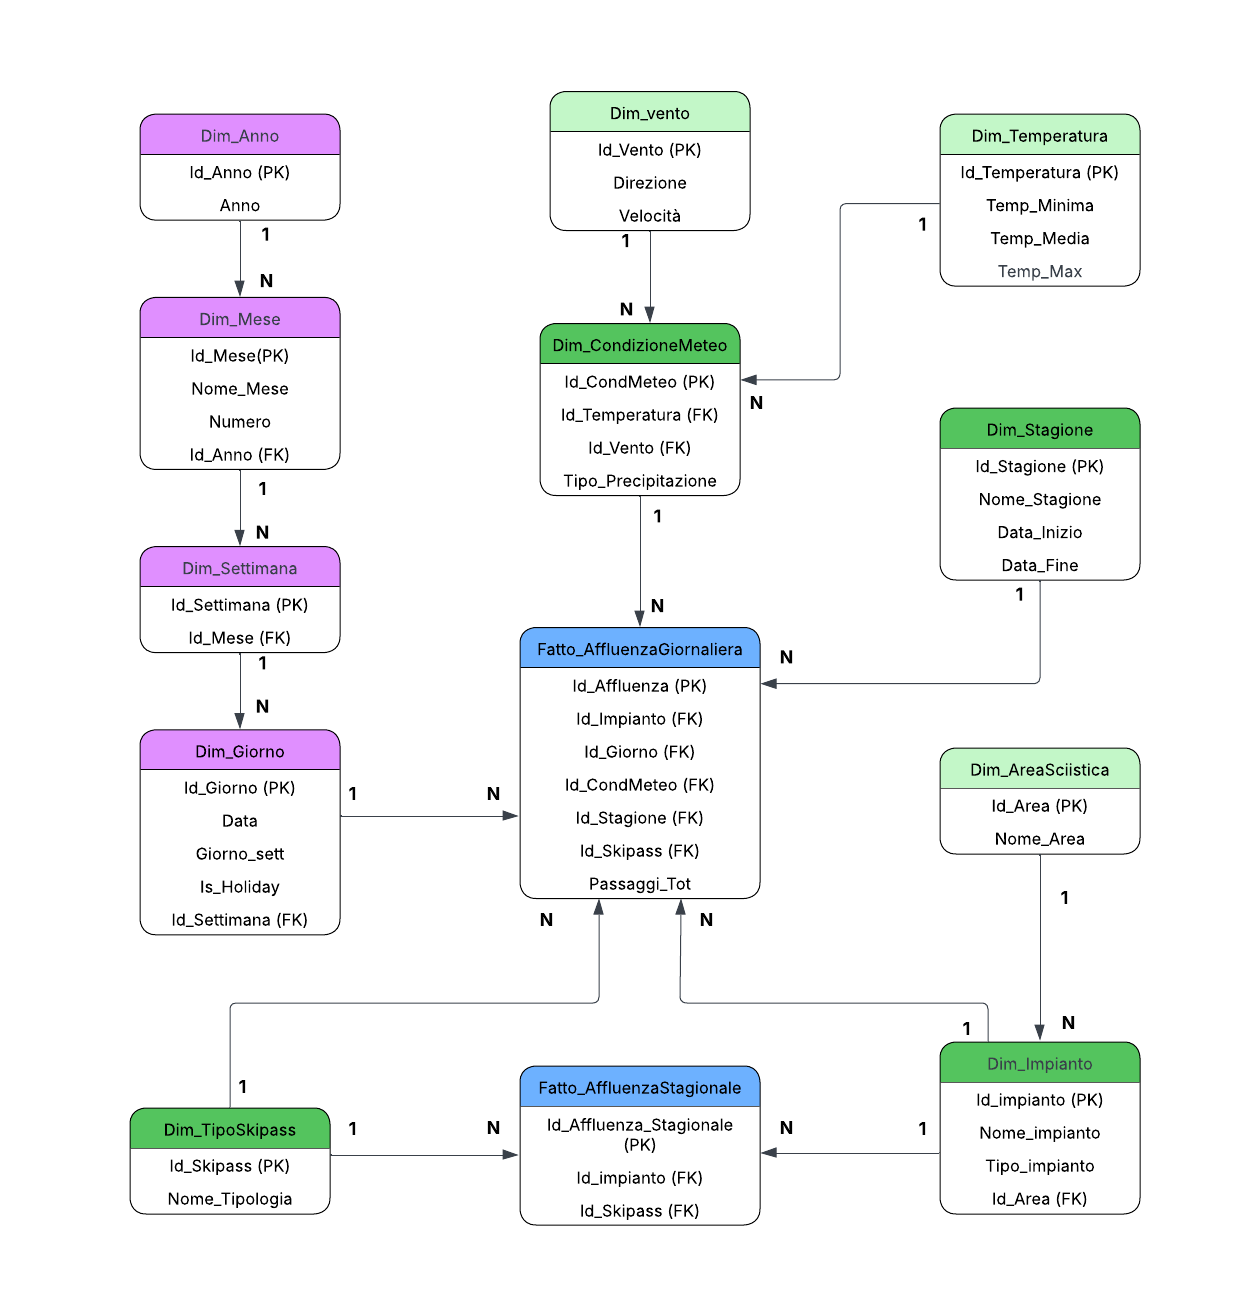
\includegraphics[width=0.9\textwidth]{images/Modello_relazionale/Constellation_Schema.png}
    \caption{Schema logico a costellazione dei fatti del dominio di analisi.}
    \label{fig:fact_constellation}
\end{figure}



\noindent
\textbf{Legenda e convenzioni dello schema.}  
Nello schema logico riportato in Figura~\ref{fig:fact_constellation}, le sigle \textbf{PK} e \textbf{FK} indicano rispettivamente le Primary Key (chiavi primarie) e le Foreign Key (chiavi esterne) delle tabelle.  
Le chiavi primarie identificano in modo univoco ciascun record all’interno della tabella, mentre le chiavi esterne stabiliscono le relazioni con le altre entità del modello, garantendo l’integrità referenziale del database.
La \textbf{cardinalità} delle relazione è sempre \textbf{1-N} nella direzione delle tabelle dei fatti, come da convezione per lo schema a costellazione.\\

È opportuno precisare che le chiavi primarie non erano presenti nei dataset originali forniti dalle aziende, ma sono state introdotte artificialmente durante la fase di progettazione logica per consentire un’identificazione univoca dei record e assicurare la coerenza del modello relazionale.  
Questa scelta è comune nella modellazione concettuale dei dati e rappresenta una buona pratica per la costruzione di schemi complessi come quelli multidimensionali.\\


Inoltre le etichette delle tabelle dei fatti e dimensionali hanno colorazioni per evidenziarne le differenze seguono la legenda sottostante \ref{fig:uml_legend}.

\begin{figure}[h]
    \centering
    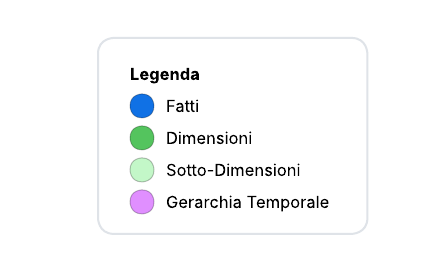
\includegraphics[width=0.4\textwidth]{images/Modello_relazionale/Legenda_Schema.png}
    \caption{Legenda UML adottata nello schema logico}
    \label{fig:uml_legend}
\end{figure}

La comprensione delle convenzioni grafiche e delle chiavi utilizzate consente ora di analizzare nel dettaglio la struttura del modello, a partire dalle \textbf{Tabelle dei Fatti}, che costituiscono il nucleo centrale della costellazione, per poi proseguire con la descrizione delle \textbf{Tabelle Dimensionali} e delle rispettive gerarchie di riferimento.\\

\subsection{Tabelle dei Fatti}

Il modello, come illustrato nel capitolo precedente, si articola attorno a due fatti principali, \textbf{Fatto\_AffluenzaGiornaliera} e \textbf{Fatto\_AffluenzaStagionale}, che  rendono necessario l'impiego di uno schema a costellazione.
Questra struttura consente di rappresentare il fenomeno dell'affluenza turistica con granularità temporali differenti (giornaliera e stagionale), mantenendo la coerenza delle relazioni tra le dimensioni e garantendo una visione integrata del dominio analizzato.


\paragraph{Fatto\_AffluenzaGiornaliera}
Rappresenta il cuore del modello dal punto di vista operativo, registrando i dati elementari relativi all'affluenza quotidiana sulle piste da sci.
Ogni record descrive un evento giornaliero, identificato da un insieme di chiavi esterne che consentono di recuperare i record correlati nelle varie dimensioni:
\textbf{Id\_Giorno}, \textbf{Id\_Impianto}, \textbf{Id\_Skipass}, \textbf{Id\_CondMeteo} e \textbf{Id\_Stagione}.
La misura quantitativa principale è rappresentata da \textbf{Passaggi\_Tot}, che indica il numero complessivo di passaggi ai tornelli degli skipass avvenuti in quella specifica giornata.
Questa tabella consente analisi ad alta risoluzione temporale e confronti mirati tra impianti, giornate e condizioni meteorologiche, fornendo una base di dettaglio per successive aggregazioni stagionali.

\paragraph{Fatto\_AffluenzaStagionale}
La seconda tabella dei fatti contiene dati aggregati su base stagionale, ottenuti tramite operazioni di sintesi (roll-up) sulla tabella giornaliera.
Le sue chiavi esterne principali (\textbf{Id\_Impianto}, \textbf{Id\_SKipass}, \textbf{Id\_Stagione}) riflettono la struttura comune condivisa con la tabella giornaliera, consentendo l'integrazione tra i due livelli di granularità temporale.
Le misure in essa contenute descrivono i volumi complessivi di passaggi e altri indicatori aggregati relativi all'intera stagione sciistica, permettendo lo studio comparativo su scala pluristagionale e l'analisi di trend evolutivi nel tempo.

\subsection{Tabelle Dimensionali}

Le tabelle dimensionali forniscono il contesto descrittivo necessario per interpretare correttamente le misure quantitative.
Nel modello a costelazione, tali dimensioni possono essere condivise da più fatti riducendo la ridondanza dei dati, migliorando la chiarezza semantica e la coerenza logica dell'intero schema. 

\paragraph{Dimensioni temporali}
Il dominio temporale è strutturato secondo più livelli gerarchici per supportare le operazioni OLAP di aggregazione e disaggregazione:

\begin{itemize}
    \item \textbf{Dim\_Giorno}: rappresenta il livello di dettaglio maggiore nella gerarchia; contiene attributi quali la data, il nome del giorno settimanale e un indicatore di festività (Is\_Holiday).
    \item \textbf{Dim\_Settimana}: collega i giorni ai rispettivi intervalli settimanali, fondamentale per valutare l'affluenza nei periodi di alta stagione.
    \item \textbf{Dim\_Mese} e \textbf{Dim\_Anno}: rappresentano i livelli superiori di aggregazione, permettono la maggiore comprensione dei cicli stagionali e delle variazioni di affluenza nel lungo periodo.
\end{itemize}

\paragraph{Dim\_Impianto}
Descrive le caratteristiche strutturali e operative di ciascun impianto di risalita\footnote{Nel modello, anche i passaggi al parcheggio della Freccia nel Cielo vengono trattati come un impianto, al fine di uniformare la struttura analitica}. Gli attributi principali includono \textbf{Nome\_Impianto} e \textbf{Tipo\_Impianto} (es. funivia, cabinovia, seggiovia, ecc.).
Ogni impianto  è inoltre associato a un'area sciistica mediante una relazione di cardinalità \textbf{1-N} con la dimensione \textbf{Dim\_AreaSciistica}, che consente, in prospettiva futura, di ampliare l’analisi a ulteriori comprensori sciistici di Cortina o di altre località dolomitiche, permettendo l’aggregazione per aree geografiche omogenee.

\paragraph{Dim\_TipoSkipass}
Contiene le informazioni relative alle diverse tipologie di Skipass 
che passano al tornello ( es. Dolomiti Superski, Di valle, Agevolati).
Questa dimensione consente di analizzare l'affluenza in relazione al tipo di titolo di accesso, offrend un punto di vista gestionale e commerciale utile alla definizione di strategie tariffarie e politiche di vendita.

\paragraph{Dim\_Stagione}
Fornisce le informazioni descrittive relative alle stagioni invernali comprese nel periodo di osservazione.
Include attributi quali il nome della stagione, la data di inizio e la data di fine, permettendo di aggregare e confrontare le performance stagionali su base cronologica.
La dimensione è strettamente collegata alla tabella dei fatti stagionale, di cui costituisce la chiave logica di riferimento temporale.

\paragraph{Dim\_CondizioneMeteo, Dim\_Temperatura e Dim\_Vento}
Queste tre dimensioni sono utilizzate per descrivere le condizioni atmosferiche prevalenti in una giornata, che influenzano in modo diretto i flussi di affluenza.
\textbf{Dim\_Temperatura} contiene i valori di temperatura minima, media e massima registrati nella giornata.
\textbf{Dim\_Vento} contiene le misurazioni della velocità e direzione del vento.\\

\textbf{Dim\_CondizioneMeteo} integra le precedenti sottodimensioni attraverso le relative chiavi esterne, aggiungendo un attributo relativo al tipo di precipitazione (pioggia, neve o assenza di fenomeni).
Queste dimensioni consentono un’analisi multidimensionale che combina variabili meteorologiche e comportamentali, evidenziando la correlazione tra condizioni climatiche e livelli di affluenza giornaliera.

In sintesi, il modello a costellazione sviluppato integra in modo coerente le diverse dimensioni del dominio: temporale, geografica, meteorologica e gestionale; in un unico sistema analitico, garantendo la precisione dell’analisi giornaliera e la completezza delle valutazioni stagionali.
Tale architettura costituisce la base logica per le successive fasi di visualizzazione e interpretazione dei dati, presentate nel capitolo dedicato alle dashboard analitiche.\\


Per completezza, si riporta in Appendice \ref{appendix:sql} lo script SQL contenente la definizione fisica del database e un esempio di popolamento dei dati, utile per la riproduzione e la verifica del modello relazionale sviluppato.



    %Data analisi e Visualizzazione

    %capitolo prova 
    \chapter{Analisi e Visualizzazione dei Dati}
\label{cha:Analisi}

Lo scopo di questo capitolo è presentare e discutere i risultati dell’analisi multidimensionale dei dati di affluenza sugli impianti sciistici gestiti da Freccia nel Cielo.
L’analisi è stata condotta mediante l’utilizzo dello strumento di Data Visualization \textbf{Tableau} \cite{Tableau}, che ha permesso di integrare il modello a costellazione dei dati in un ambiente interattivo capace di evidenziare le diverse dimensioni informative rilevanti per lo studio.\\

I risultati sono presentati sotto forma di dashboard analitiche, illustrate nel seguito del capitolo, che supportano l’indagine dei casi di studio individuati.
L’approccio combina tecniche di analisi descrittiva e comparativa, con l’obiettivo di individuare pattern ricorrenti e potenziali trend inaspettati all’interno del dataset.\\

Per strutturare l’esposizione dei risultati in maniera sistematica, l’analisi è stata organizzata attorno a un insieme di domande guida, concepite per enfatizzare gli aspetti più rilevanti dello studio sia per il contesto territoriale di Cortina d’Ampezzo, sia per la società impiantistica considerata.

Ogni domanda è affrontata mediante una o più visualizzazioni, sviluppate utilizzando sia i campi originali del dataset sia campi calcolati dedicati, con lo scopo di fornire risposte chiare e supportate dai dati. Le dashboard presentate includono filtri interattivi, sistemi di selezione, differenti tipologie grafiche e operazioni OLAP\footnote{Tali operazioni, tra cui roll-up, drill-down, slicing e dicing, sono state discusse nei capitoli precedenti.}, garantendo un’esplorazione dinamica ed esaustiva delle informazioni disponibili.\\

Le principali domande a cui si intende rispondere sono:

\begin{enumerate}
    \item \textbf{Analisi 1 – Picchi di affluenza stagionale}~(\ref{sec:analisi1}):  
    In quali periodi della stagione invernale si registrano i massimi livelli di affluenza agli impianti, e come si distribuiscono i picchi di passaggi in corrispondenza dei diversi periodi festivi (Natale, Carnevale, ordinario)?

    \item \textbf{Analisi 2 – Variazioni settimanali e pattern giornalieri}~(\ref{sec:analisi2}):  
    Quali variazioni si osservano nei livelli di affluenza tra i diversi giorni della settimana, in particolare tra venerdì, sabato e domenica, e quali tendenze emergono nel confronto cumulativo dei passaggi?

    \item \textbf{Analisi 3 – Classificazione e influenza delle condizioni meteorologiche}~(\ref{sec:analisi3}):  
    In che modo le condizioni atmosferiche, e in particolare la temperatura percepita e l’escursione termica giornaliera, caratterizzano l’andamento della stagione sciistica e la distribuzione delle giornate nelle diverse categorie termiche?

    \item \textbf{Analisi 4 – Impatto delle giornate nevose sulle tipologie di skipass}~(\ref{sec:analisi4}):  
    Qual è l’effetto delle giornate con precipitazioni nevose sull’affluenza complessiva e sull’utilizzo delle diverse tipologie di skipass (Valle e Dolomiti Superski), e come varia tale impatto nel corso della stagione?
\end{enumerate}


Le sezioni seguenti approfondiscono ciascuna di queste domande, presentando le dashboard costruite e i relativi indicatori calcolati, accompagnati da un commento interpretativo volto a evidenziare le tendenze emerse e la loro rilevanza per la gestione turistica e operativa della località.

\newpage

%-----------------------------------------
\section{Campi calcolati e parametri su Tableau}

Prima di procedere all’analisi delle domande chiave, è opportuno evidenziare che, per supportare la lettura e l’interpretazione dei dati, nell’ambiente Tableau sono stati sviluppati diversi parametri e campi calcolati. Tali componenti hanno contribuito a migliorare la chiarezza delle visualizzazioni e l’efficacia analitica delle dashboard.

Nel seguito vengono illustrati alcuni tra i principali campi calcolati adottati; ulteriori elementi non esplicitamente descritti in questa sezione saranno comunque richiamati, ove necessario, durante l’analisi dei grafici.\footnote{La lista completa dei campi calcolati è riportata negll'appendice.}



\subsection*{Classificazione Periodo Festivo}
Di seguito viene presentato il campo calcolato che permette la distinzione del periodo festivo nel corso della stagione, grazie a un range di date fissato.

\begin{lstlisting}[language=SQL, caption={Campo calcolato: Classificazione periodo festivo}]
IF [Data] >= DATE("2023-12-24") AND [Data] <= DATE("2024-01-06") THEN "Natale"
ELSEIF [Data] >= DATE("2024-02-08") AND [Data] <= DATE("2024-02-17") THEN "Carnevale"
ELSE "Ordinario"
END
\end{lstlisting}

Questo campo consente di identificare e visualizzare i principali periodi festivi della stagione invernale, tipicamente associati a un aumento dell’affluenza agli impianti sciistici. La classificazione è applicata a tutte le stagioni analizzate, adattando gli intervalli temporali in base al calendario di ciascun anno.\\

In particolare, il periodo di \textbf{Carnevale} non presenta date fisse e viene quindi delimitato considerando il Giovedì Grasso come data di inizio e il weekend del Carnevale Ambrosiano come data conclusiva. Tale scelta riflette le differenze territoriali nelle festività, che possono influenzare i flussi turistici e le decisioni di viaggio degli utenti provenienti da diverse aree geografiche.\\

Il periodo \textbf{Natalizio}, invece, presenta una maggiore stabilità temporale: esso decorre convenzionalmente dal 24 dicembre fino al 6 gennaio, con una possibile estensione di uno o due giorni in funzione della collocazione dell’ultimo weekend festivo della stagione. Questa delimitazione consente di catturare in modo più realistico le dinamiche turistiche legate alle festività di fine anno, tradizionalmente caratterizzate da un afflusso particolarmente elevato.

\subsection*{Classificazione Categoria Temperatura} \label{subsec:Cat_temperatura}
Un ulteriore gruppo di campi calcolati è stato sviluppato per classificare le giornate in base alla temperatura percepita sulle piste da sci. Tale classificazione consente di valutare l'effetto congiunto della temperatura e del vento, fattori che incidono direttamente sul comfort degli utenti e potenzialmente sulla loro propensione a frequentare gli impianti.

Il primo campo necessario definisce la temperatura base, ovvero il valore termico utilizzato come riferimento per l’analisi. Questo campo agisce come selettore e consente di scegliere tra le temperature minima e media, escludendo la temperatura massima in quanto raramente rappresentativa delle condizioni percepite dagli sciatori durante la giornata, risultando quindi poco significativa ai fini dell’analisi.
Il valore predefinito è impostato sulla temperatura media, in quanto più indicativa dell’intervallo orario in cui gli impianti sono operativi e dell’esperienza termica complessiva sulle piste.\\

A partire dalla temperatura base , viene calcolata la \textbf{Temperatura Percepita}, integrando l'effetto del vento, se la sua velocità è maggiore di una certa soglia, mediante l'applicazione di una formula riconducibile all'indice \textbf{Wind Chill}, che consente di stimale la diminuizione della percezione della temperatura in presenza di forte ventilazione.\\

Infine sulla base della temperatura percepita viene generato il campo \textbf{Categoria Temperatura} presentato di seguito, che classifica ciascuna giornata in fasce qualitative (ad es. Freddo, Mite, Caldo). Questa categorizzazione favorisce un’interpretazione immediata delle condizioni climatiche delle giornate e permette di analizzarne l’impatto potenziale sui flussi di utenza.
Si noti che anche in questo campo è presente un controllo sull'intensità del vento, questo per considerare alcuni casi in cui, pur non verificandosi pienamente le condizioni per l'applicazione formale dell'indice, la presenza di vento sostenuto determini comunque una percezione soggettiva più rigida.\\


\begin{lstlisting}[language=SQL, caption={Campo calcolato: Categoria Temperatura}]
IF ISNULL([Temp Percepita]) THEN
    "Missing"
ELSEIF [Temp Percepita] < 2 THEN
    "Freddo"
ELSEIF [Temp Percepita] <= 8 
   AND [Velocita vento  (m/s)] >= 4 THEN
    "Freddo"
ELSEIF [Temp Percepita] <= 12 THEN
    "Mite"
ELSE
    "Caldo"
END
\end{lstlisting}

Si evidenzia che i campi calcolati \textbf{Temperatura Base} e \textbf{Temperatura Percepita} sono riportati integralmente in Appendice ai seguenti riferimento \ref{appendix:Temp_Base}. 

\subsection*{Parametri}

Oltre ai campi calcolati, Tableau consente di definire dei \textbf{parametri}, ovvero elementi dinamici che fungono da selettori di valore e permettono di rendere interattive le visualizzazioni.  
Un parametro può assumere uno o più valori predefiniti, di cui uno è impostato come valore di default visualizzato all’apertura della dashboard.  
La modifica del parametro da parte dell’utente comporta l’aggiornamento immediato dei grafici e dei campi calcolati collegati, consentendo così una lettura flessibile e personalizzabile dei dati.

Di seguito sono riportati i principali parametri utilizzati nelle dashboard:

\begin{itemize}
    \item \textbf{Selezione Skipass}: consente di scegliere la tipologia di skipass da utilizzare nei calcoli relativi ai passaggi.  
    I valori disponibili sono: All (tutti i titoli), DS (Dolomiti Superski) e Valle (skipass locale).  
    La selezione del parametro influisce su tutte le viste collegate, aggiornando dinamicamente le misure e i grafici.
    
    \item \textbf{Tipo Temperatura}: determina quale valore termico viene impiegato nei campi calcolati meteorologici, permettendo di scegliere tra la temperatura minima e la temperatura media.  
    Questa opzione consente di confrontare le diverse metodologie di calcolo della temperatura percepita, valutandone l’impatto sulle analisi climatiche e di affluenza.
\end{itemize}

nel seguito vengono presentate le analisi condotte sulla base delle domande guida elencate all'inizio di questo capitolo.


%-----------------------------------------
\section{Analisi 1 – Picchi di affluenza stagionale}\label{sec:analisi1}

La prima analisi condotta ha l’obiettivo di individuare i periodi della stagione sciistica caratterizzati dai livelli più elevati di affluenza. Tale indagine costituisce il punto di partenza naturale dello studio, poiché la periodizzazione degli accessi rappresenta una variabile chiave che influenzerà anche le analisi successive, in particolare per quanto riguarda le festività e i flussi turistici associati.\\

Per rispondere a questa domanda è stata realizzata una \textbf{dashboard} che mostra l’andamento dei \textbf{passaggi totali giornalieri} registrati su tutti gli impianti del comprensorio \textit{Freccia nel Cielo} nel corso della stagione 2023–24.  
La vista principale consente di individuare visivamente i picchi di affluenza e di distinguere i periodi festivi grazie all’applicazione del campo calcolato “\textbf{Periodo Festivo}”, descritto in precedenza, che assegna una colorazione diversa alle giornate appartenenti alle festività di \textbf{Natale} e \textbf{Carnevale}, uniche rilevanti per l’arco stagionale considerato.\\

La vista secondaria, invece, mostra il \textbf{cumulativo dei passaggi} per ciascun periodo festivo, consentendo un confronto immediato tra le tre categorie considerate (Ordinario, Natale, Carnevale).  
Di seguito è riportata la visualizzazione complessiva nella figura~\ref{fig:passaggi_tot_stagione}.



%Grafico qui
\begin{figure}[htbp]
    \centering
    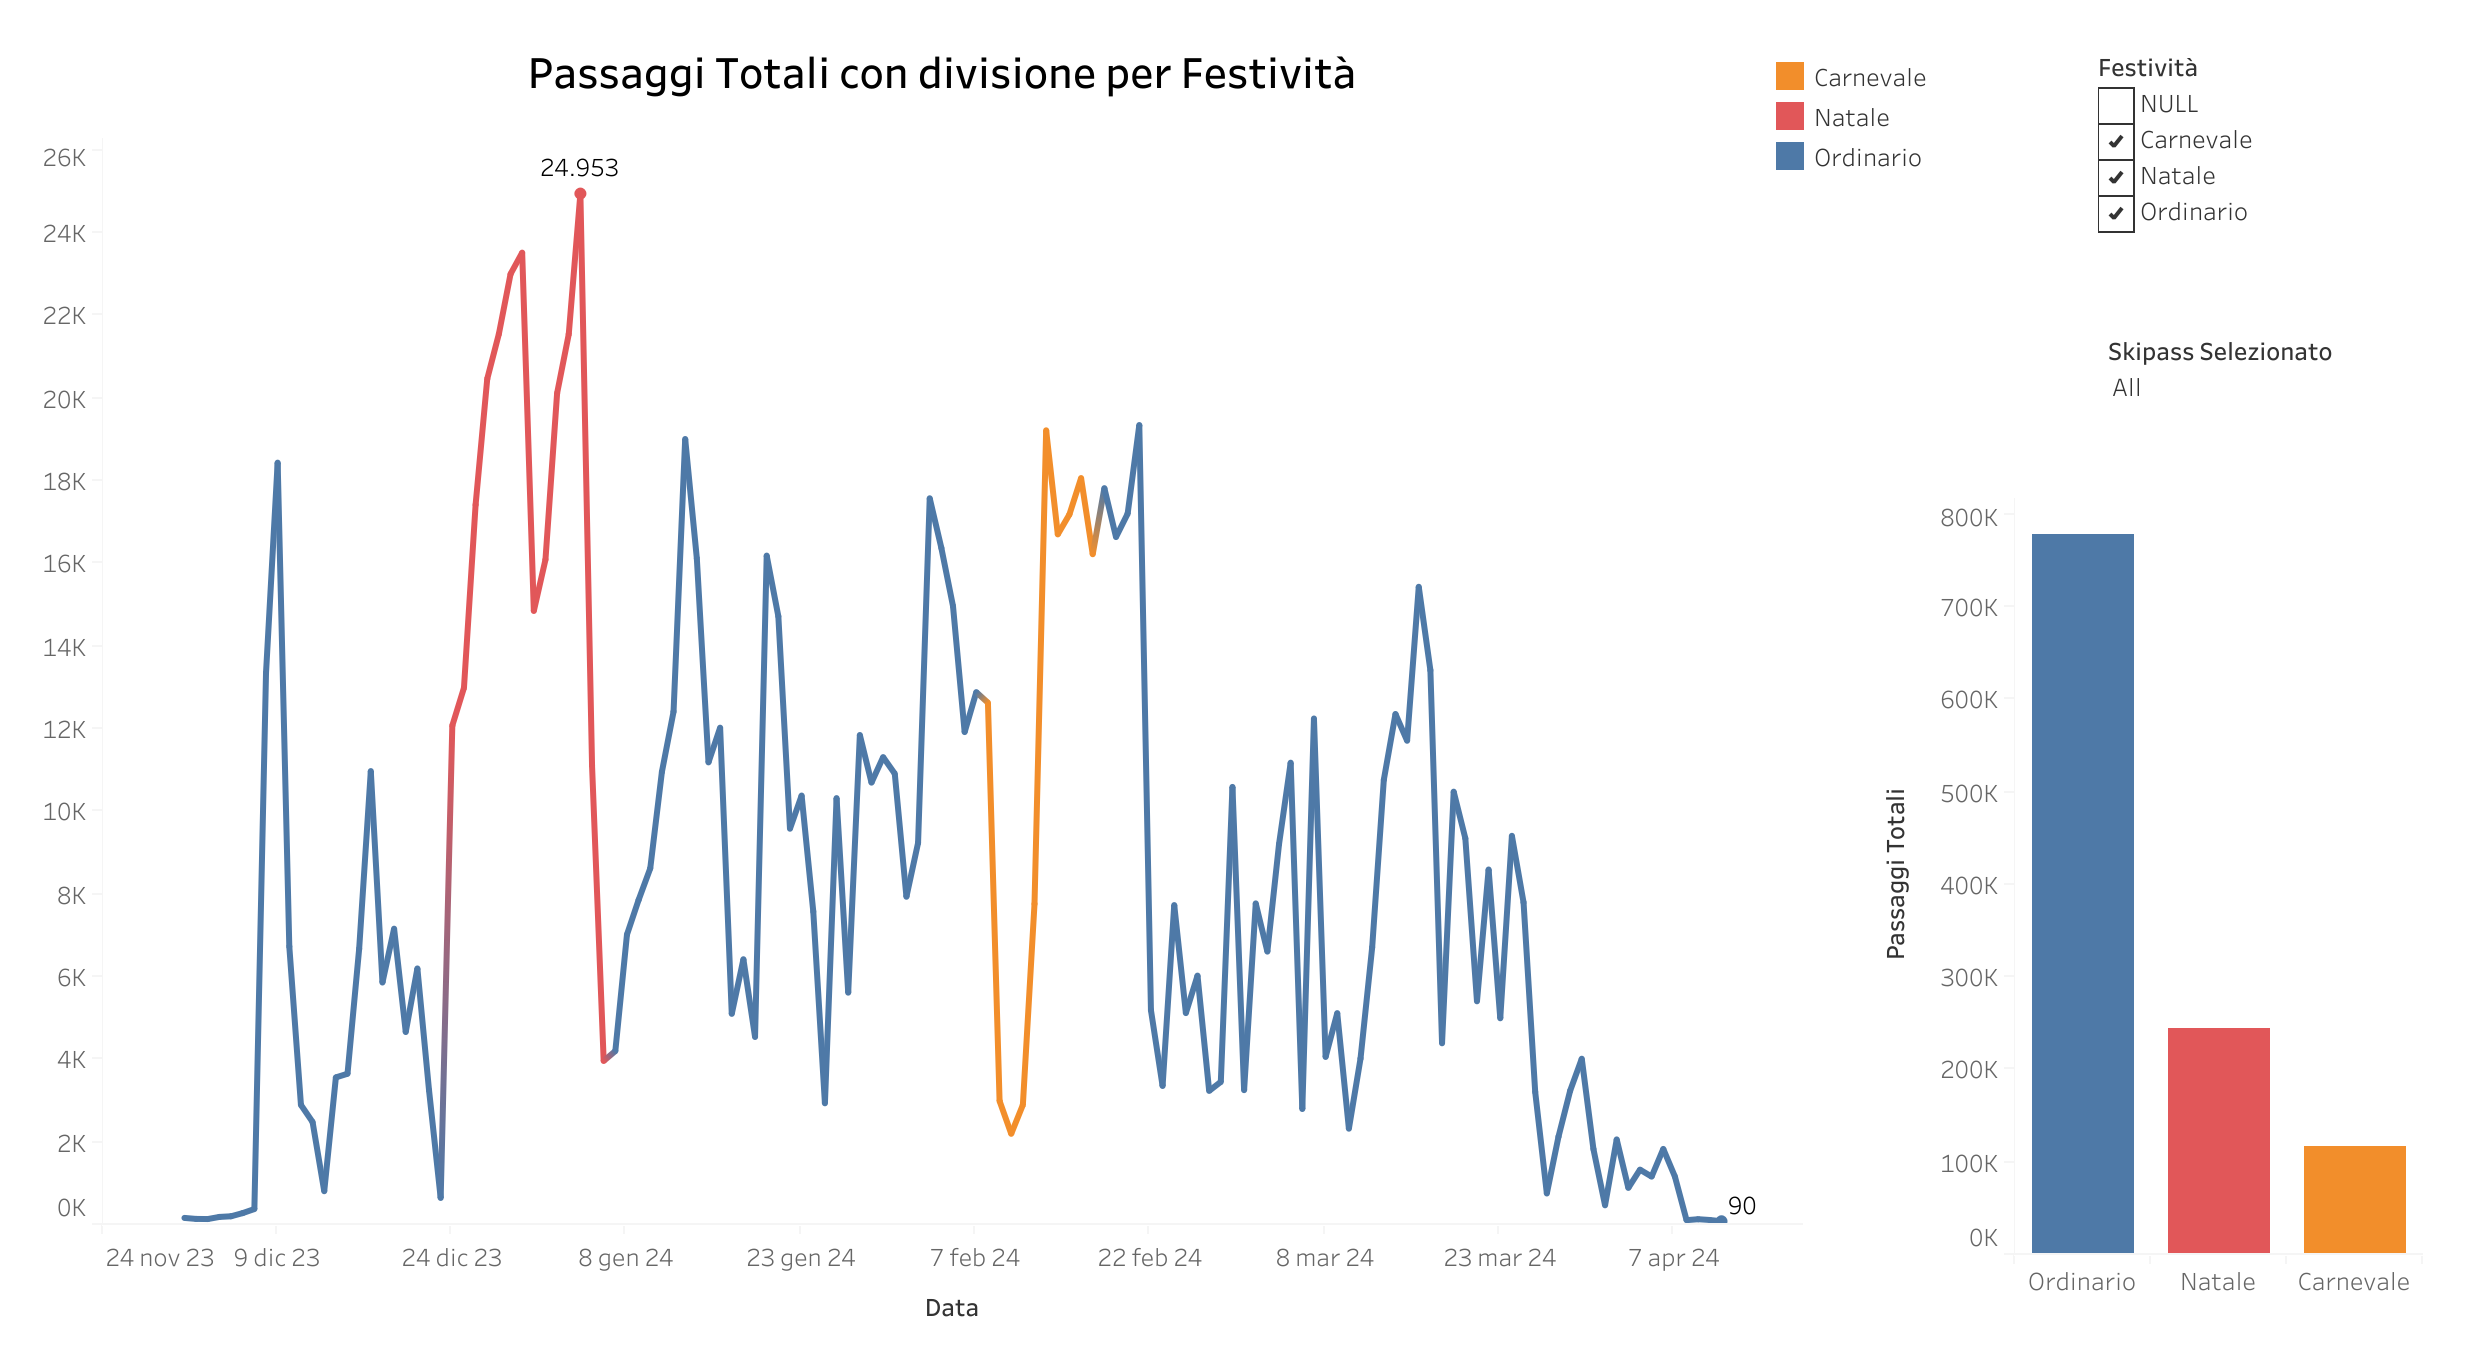
\includegraphics[width=0.95\textwidth]{images/Tableau/Studio_1/Passaggi Totali.png}
    \caption{Andamento giornaliero dei passaggi totali nella stagione 2023–24, suddivisi per periodo festivo.}
    \label{fig:passaggi_tot_stagione}
\end{figure}



Per ampliare la lettura temporale dei dati è stata inoltre introdotta una vista alternativa che applica un’operazione di \textbf{Roll-Up} sulla dimensione temporale, aggregando i dati a livello \textbf{settimanale}.  
Questa trasformazione consente di valutare l’evoluzione dei flussi in un periodo di tempo più ampio e di cogliere con maggiore chiarezza gli effetti successivi alle festività.  
La figura~\ref{fig:passaggi_tot_settimana} mostra l’andamento settimanale dei passaggi totali, evidenziando i trend di continuità e di ripresa post-festiva.


\paragraph{Struttura della visualizzazione e variabili impiegate}
\begin{itemize}
    \item \textbf{Asse X}: Nella vista principale rappresenta la Data, con possibile operazione di Roll-up lungo la gerarchia per aumentare la granularità (giorno \textrightarrow  settimana \textrightarrow  mese); nella vista secondaria riporta invece le tre tipologie di periodo festivo.
    \item \textbf{Asse Y}:  per entrambe le viste è costituito dai \textbf{passaggi totali}, calcolati sul totale o filtrati in base alla tipologia di skipass selezionata tramite il parametro \textbf{Skipass Selezionato}, che consente di visualizzare i dati complessivi (All) o solo quelli relativi ai titoli  “ di Valle” e “Dolomiti Superski”, il tutto è incluso nel campo calcolato \textbf{Tipo SKipass} presente nell'appendice \ref{appendix:tipo_skipass}.
    \item \textbf{Filtri e colorazione}: Campo calcolato “Periodo Festivo”, utilizzato per evidenziare e confrontare i diversi intervalli stagionali.
    \item \textbf{Tipologia di Grafico}: lineare nella visualizzazione principale e a barre nella visualizzazione secondaria.
\end{itemize}

\paragraph{Valutazioni e osservazioni}
Dall’analisi emerge chiaramente come il \textbf{periodo natalizio} rappresenti il picco assoluto di affluenza, con il massimo registrato il \textbf{4 gennaio} (\textbf{24.953 passaggi}) (vedi \ref{fig:spec_giorno} per la specifica del giorno), in linea con le aspettative relative ai flussi turistici della località. \\

Un elemento rilevante che si può cogliere a vista d'occhio nell'analisi è relativo alla fase natalizia, che mostra un andamento fortementente \textbf{irregolare}, caratterizzato da forti oscillazioni giornaliere tra picchi molto elevati e giornate di affluenza più contenuta.
Il periodo carnevalesco, al contrario, evidenzia un comportamento più \textbf{stabile e uniforme}, mantenendo valori di affluenza alti anche nei giorni immediatamente successivi alla fine della festività.  
La media giornaliera dei passaggi tra il 13 e il 21 febbraio si attesta su circa \textbf{17.600 passaggi}, un valore molto vicino alla media registrata tra il 25 dicembre e il 6 gennaio (\textbf{17.800 passaggi}), ma con una variabilità sensibilmente inferiore.  
Ciò suggerisce una presenza turistica più regolare e distribuita nel tempo, probabilmente favorita dalla concomitanza di vacanze scolastiche e da condizioni meteorologiche più prevedibili rispetto al periodo natalizio; tramite il filtro sui periodi festivi inoltre è possibile visionare la dashboard in appendice \ref{fig:passaggi_tot_noNatale} con l'esclusione del periodo natalizio per avere un  confronto senza i picchi natalizi.

La visualizzazione con roll-up settimanale (\ref{fig:passaggi_tot_settimana}) conferma e rafforza questa lettura: la settimana centrale di Natale rappresenta il picco assoluto stagionale (\textbf{133.838 passaggi}), seguita da un progressivo calo e da una successiva ripresa durante il Carnevale.  
Dopo quest’ultimo periodo, l’andamento mostra una discesa più graduale ma costante, evidenziando come l’affluenza rimanga sostenuta anche nelle settimane successive, probabilmente grazie a condizioni di innevamento ancora favorevoli.\\

In sintesi, l’analisi mostra come il periodo natalizio, pur rimanendo il momento di massima affluenza, presenti un andamento più volatile, mentre il Carnevale rappresenta una fase di equilibrio e continuità per l’affluenza stagionale.  
Queste evidenze risultano particolarmente utili ai fini gestionali, poiché permettono di pianificare in modo differenziato le risorse e le strategie operative in funzione delle diverse dinamiche festive.

%-----------------------------------------
\section{Analisi 2 – Variazioni settimanali e pattern giornalieri}
\label{sec:analisi2}

La seconda analisi ha l'obiettivo di individuare quali giorni della settimana registrano i livelli più elevati di affluenza agli impianti. Tale valutazione risulta utile al fine di pianificare in modo più efficiente le attività operative, l'organizzazione del personale e la gestione delle risorse nelle giornate caratterizzate da maggiore pressione turistica. Questa analisi è presentata tramite una Dashboard contenente due visualizzazioni distinte.\\

 La prima analizza i \textbf{passaggi totali nei vari giorni settimanali}. Per non andare a sovraccaricare i grafici di troppe variabili, si è scelto di presentare i dati dei giorni più rilevanti in questa sezione, quindi quelle relativo ai giorni del fine settimana, confrontando \textbf{venerdì, sabato e domenica}. Questa scelta è motivata dal fatto che il weekend rappresenta, indipendentemente dalle festività, il periodo di picco ricorrente dell’affluenza turistica.

Il secondo grafico riporta invece il \textbf{totale cumulativo dei passaggi per giorno della settimana}, consentendo di valutare l’incidenza complessiva di ciascun giorno sul totale stagionale e di stimare quali giornate richiedano una maggiore capacità organizzativa.

 Di seguito in  \ref{fig:Weekend_cumulativo}  è presentata la dashboard complessiva che permette quindi una interpretazione  interattiva dei dati, grazie al filtro modificabile \textbf{Giorni selezionati}, secondo due metodologie di rappresentazione distinte ma collegate tra loro.



\begin{figure}[htbp]
    \centering
    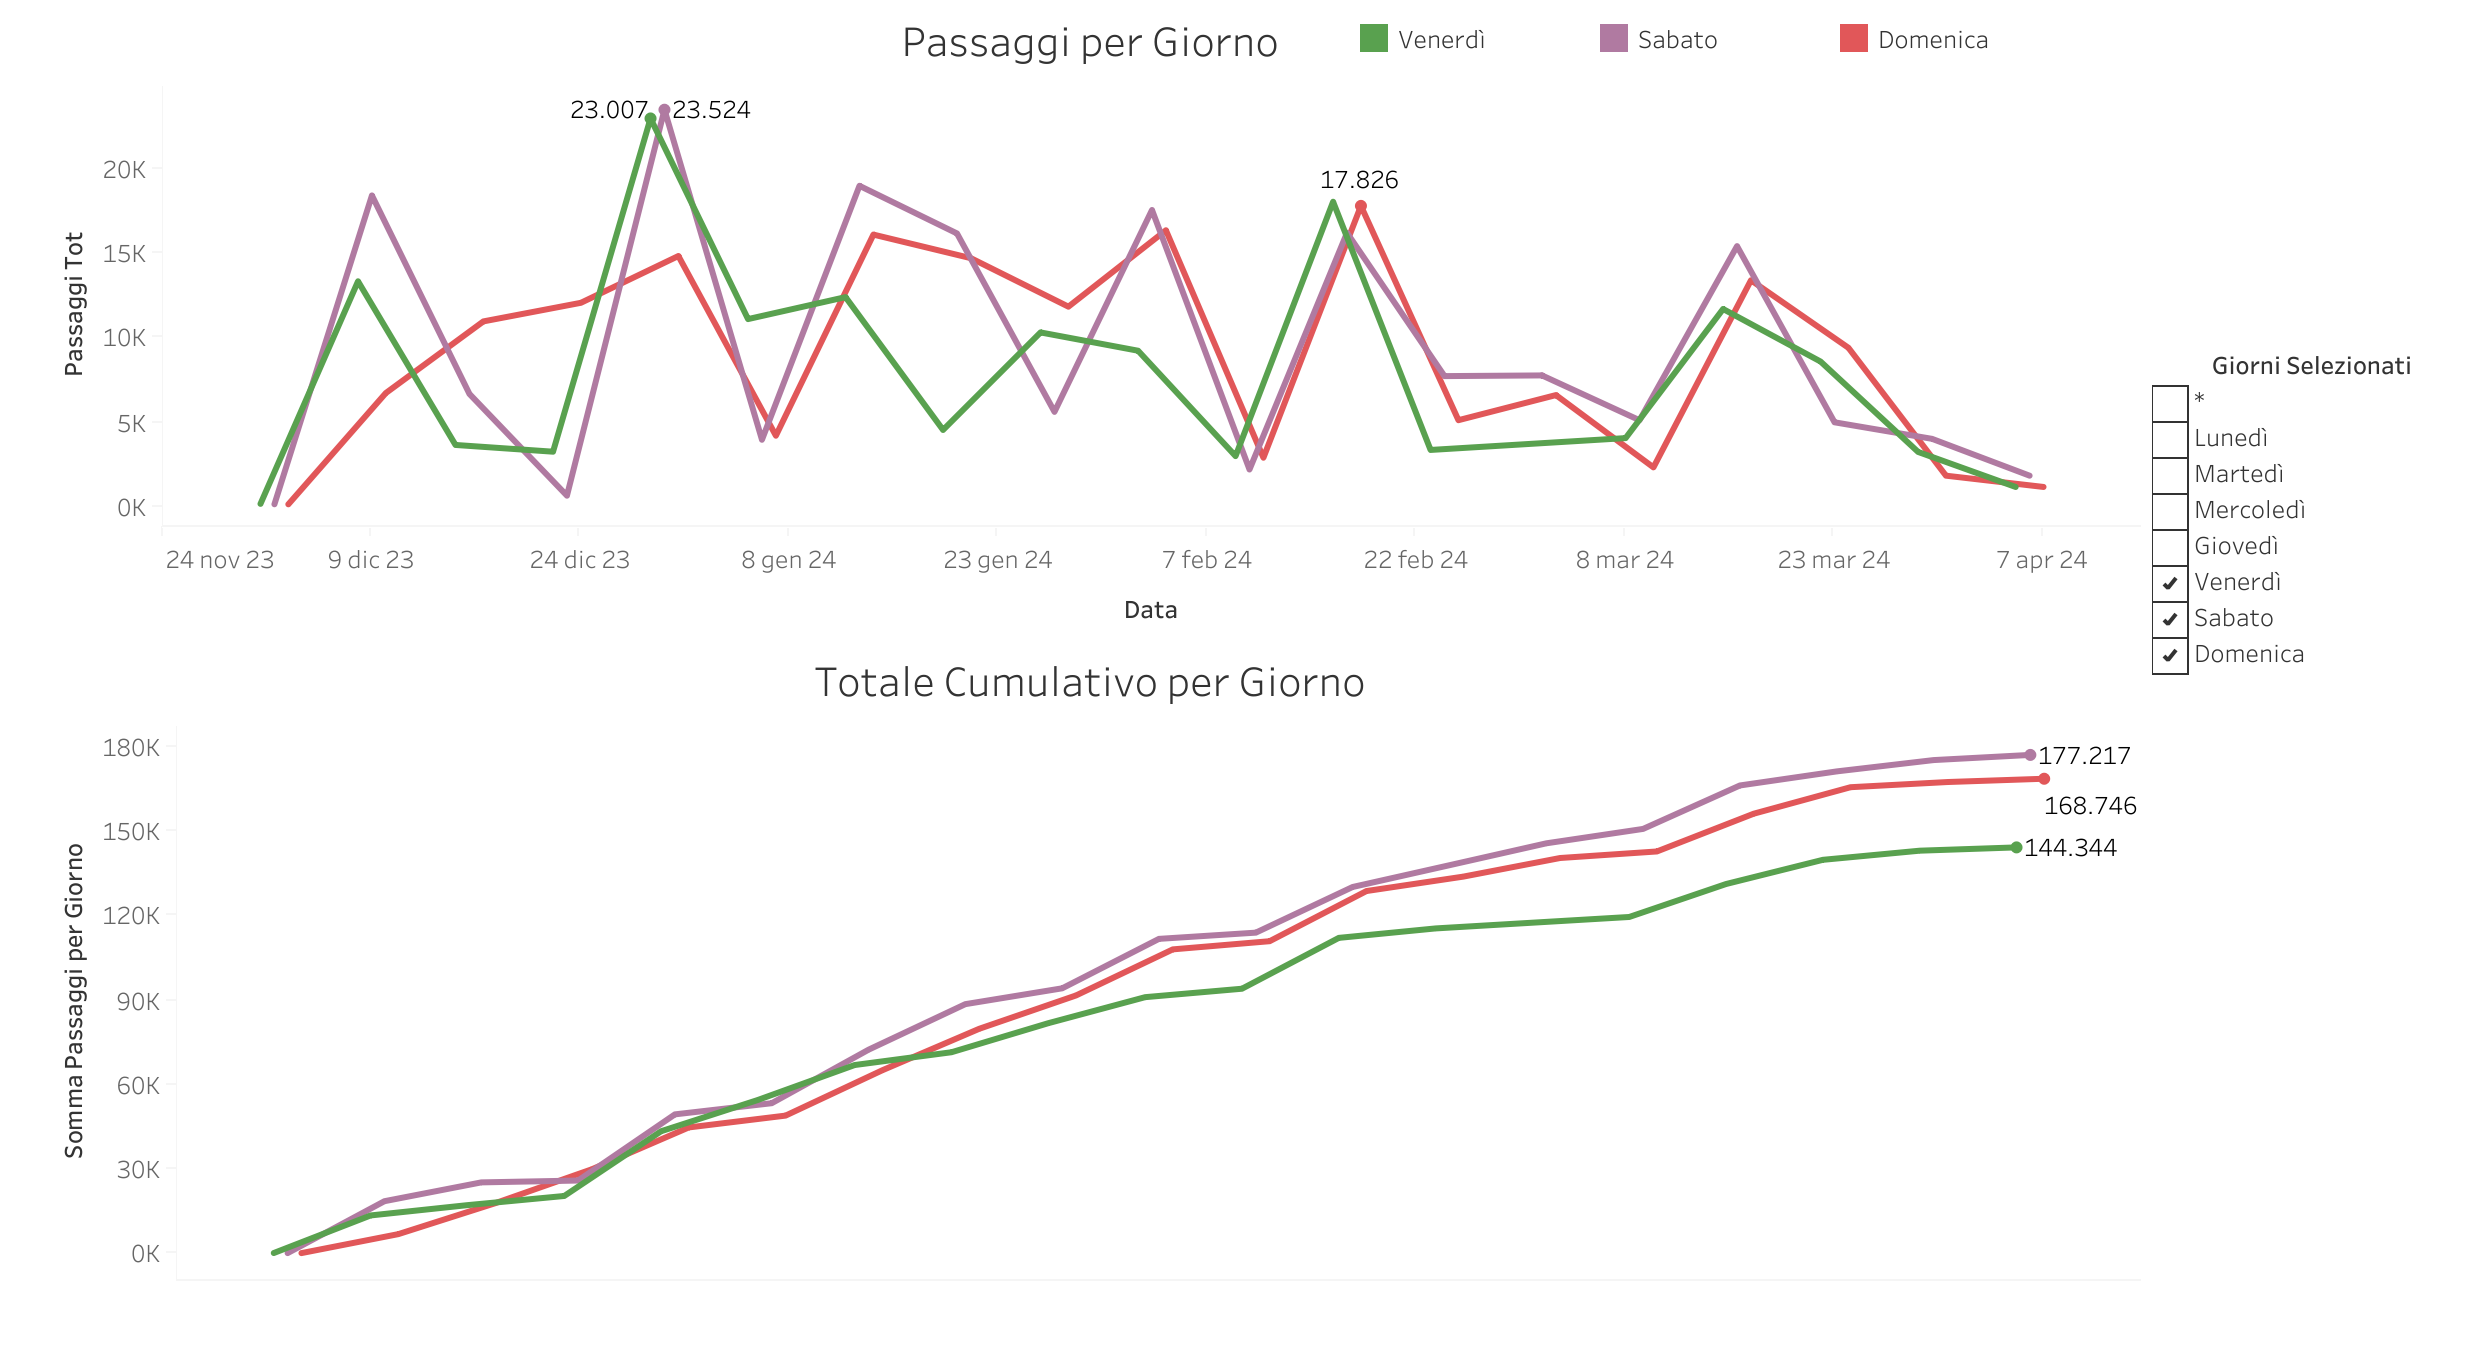
\includegraphics[width=0.95\textwidth]{images/Tableau/Studio_2/Dash_Weekend_cumulativo.png}
    \caption{Dashboard per passaggi settimanali con totale cumulativo}
    \label{fig:Weekend_cumulativo}
\end{figure}

%grafici

\paragraph{Struttura della visualizzazione e variabili Impiegate}
\begin{itemize}
    \item \textbf{Asse X}: Data (variabile continua).
    \item \textbf{Asse Y}: Passaggi totali (variabile continua); nel secondo grafico è riportato il totale corrente, calcolato come somma cumulativa dei passaggi per giorno mediante la funzione di aggregazione “Totale corrente”.
    \item \textbf{Filtri e colorazioni}:differenziazione dei giorni mediante codici colore distinti; filtro interattivo sui giorni selezionati, estendibile a tutti i giorni della settimana tramite variabili testuali.
    \item \textbf{Tipologie di grafico}: grafici lineari multipli.
\end{itemize}


\paragraph{Valutazioni e osservazioni}
Dall’analisi emerge un risultato particolarmente rilevante e, in parte, inatteso: il giorno con il maggior numero di passaggi registrati durante la stagione è il \textbf{sabato}, non solo, se si va ad analizzare il weekend si nota che la linea del sabato è in generale sempre la più alta.
Si potrebbe infatti presumere che la giornata di picco corrisponda alla \textbf{domenica}, quando le presenze turistiche raggiungono generalmente i livelli massimi. Tuttavia, nel caso di Cortina d’Ampezzo, la dinamica appare differente.
Una spiegazione di questo fenomeno può essere trovata nella conformazione geografica della valle ampezzana, che si estende come una conca chiusa avendo un'unica strada principale ad esclusione dei passi, su cui si distribuisce il traffico, induce molti visitatori a lasciare la località la domenica, preferendo rientrare anticipatamente per evitare il traffico del rientro.
Ne risulta dunque un picco di presenze nella giornata di sabato, seguito da una progressiva diminuzione dei passaggi la domenica.\\

Un ulteriore elemento interessante emerge osservando il \textbf{grafico cumulativo}: includendo gli altri giorni della settimana, si nota che, dopo il sabato, il secondo giorno con il più alto totale di passaggi non è la domenica, bensì il \textbf{martedì}.
Questo andamento, apparentemente controintuitivo, suggerisce una ripresa significativa delle attività subito dopo il lunedì, probabilmente legata a turisti in vacanza prolungata, nuove partenze settimanali e posizionameni delle festività nel calendario.
Si tratta di un’informazione di rilievo per la gestione operativa degli impianti, che possono pianificare in modo più efficiente la distribuzione delle risorse durante la settimana.

La versione estesa della dashboard, con l'ulteriore selezione del martedì, è riportata in Appendice al riferimento~\ref{fig:dash_tuesday}.


%-----------------------------------------

\section{Analisi 3 – classificazione e influenza delle Condizioni metereologiche}
\label{sec:analisi3}

Questa analisi è stata sviluppata per confrontare le condizioni meteorologiche osservate durante l’intera stagione invernale, con l’obiettivo di classificare ciascuna giornata secondo le tre categorie di temperatura definite nella sezione~\ref{subsec:Cat_temperatura}: \textbf{freddo}, \textbf{mite} e \textbf{caldo}.  \\

Nella vista principale, ogni giornata è rappresentata da una barra la cui colorazione identifica la categoria di temperatura percepita .  
L’altezza della barra è determinata da un parametro denominato \textbf{Range Size}, calcolato come la differenza tra la temperatura massima e quella minima registrata nella stessa giornata, e rappresentante quindi l’\textbf{escursione termica giornaliera}.  
Sovrapposta alle barre è tracciata una linea grigia che mostra l’andamento della \textbf{temperatura percepita} nel corso dell'intera stagione, ottenuta mediante il campo calcolato descritto in appendice~\ref{}.  
Questa combinazione a doppio asse consente di osservare simultaneamente sia la variabilità giornaliera delle temperature sia l’andamento generale percepito nel corso della stagione. \\

La vista secondaria, collocata sulla destra della dashboard, riassume invece i \textbf{passaggi totali ai tornelli} in funzione della categoria di temperatura.  
Essa consente di valutare in modo sintetico la distribuzione complessiva dell’affluenza in relazione alle diverse condizioni termiche: i valori più elevati si registrano nelle giornate classificate come “fredde”, seguite da quelle “miti”, mentre le giornate “calde” mostrano un’incidenza pressoché marginale.  
Questa rappresentazione, quindi, fornisce un quadro immediato dell’impatto delle condizioni climatiche sull’utilizzo degli impianti e permette di collegare i pattern meteorologici osservati nel grafico principale con i comportamenti di affluenza.


%grafico

\begin{figure}[htbp]
    \centering
    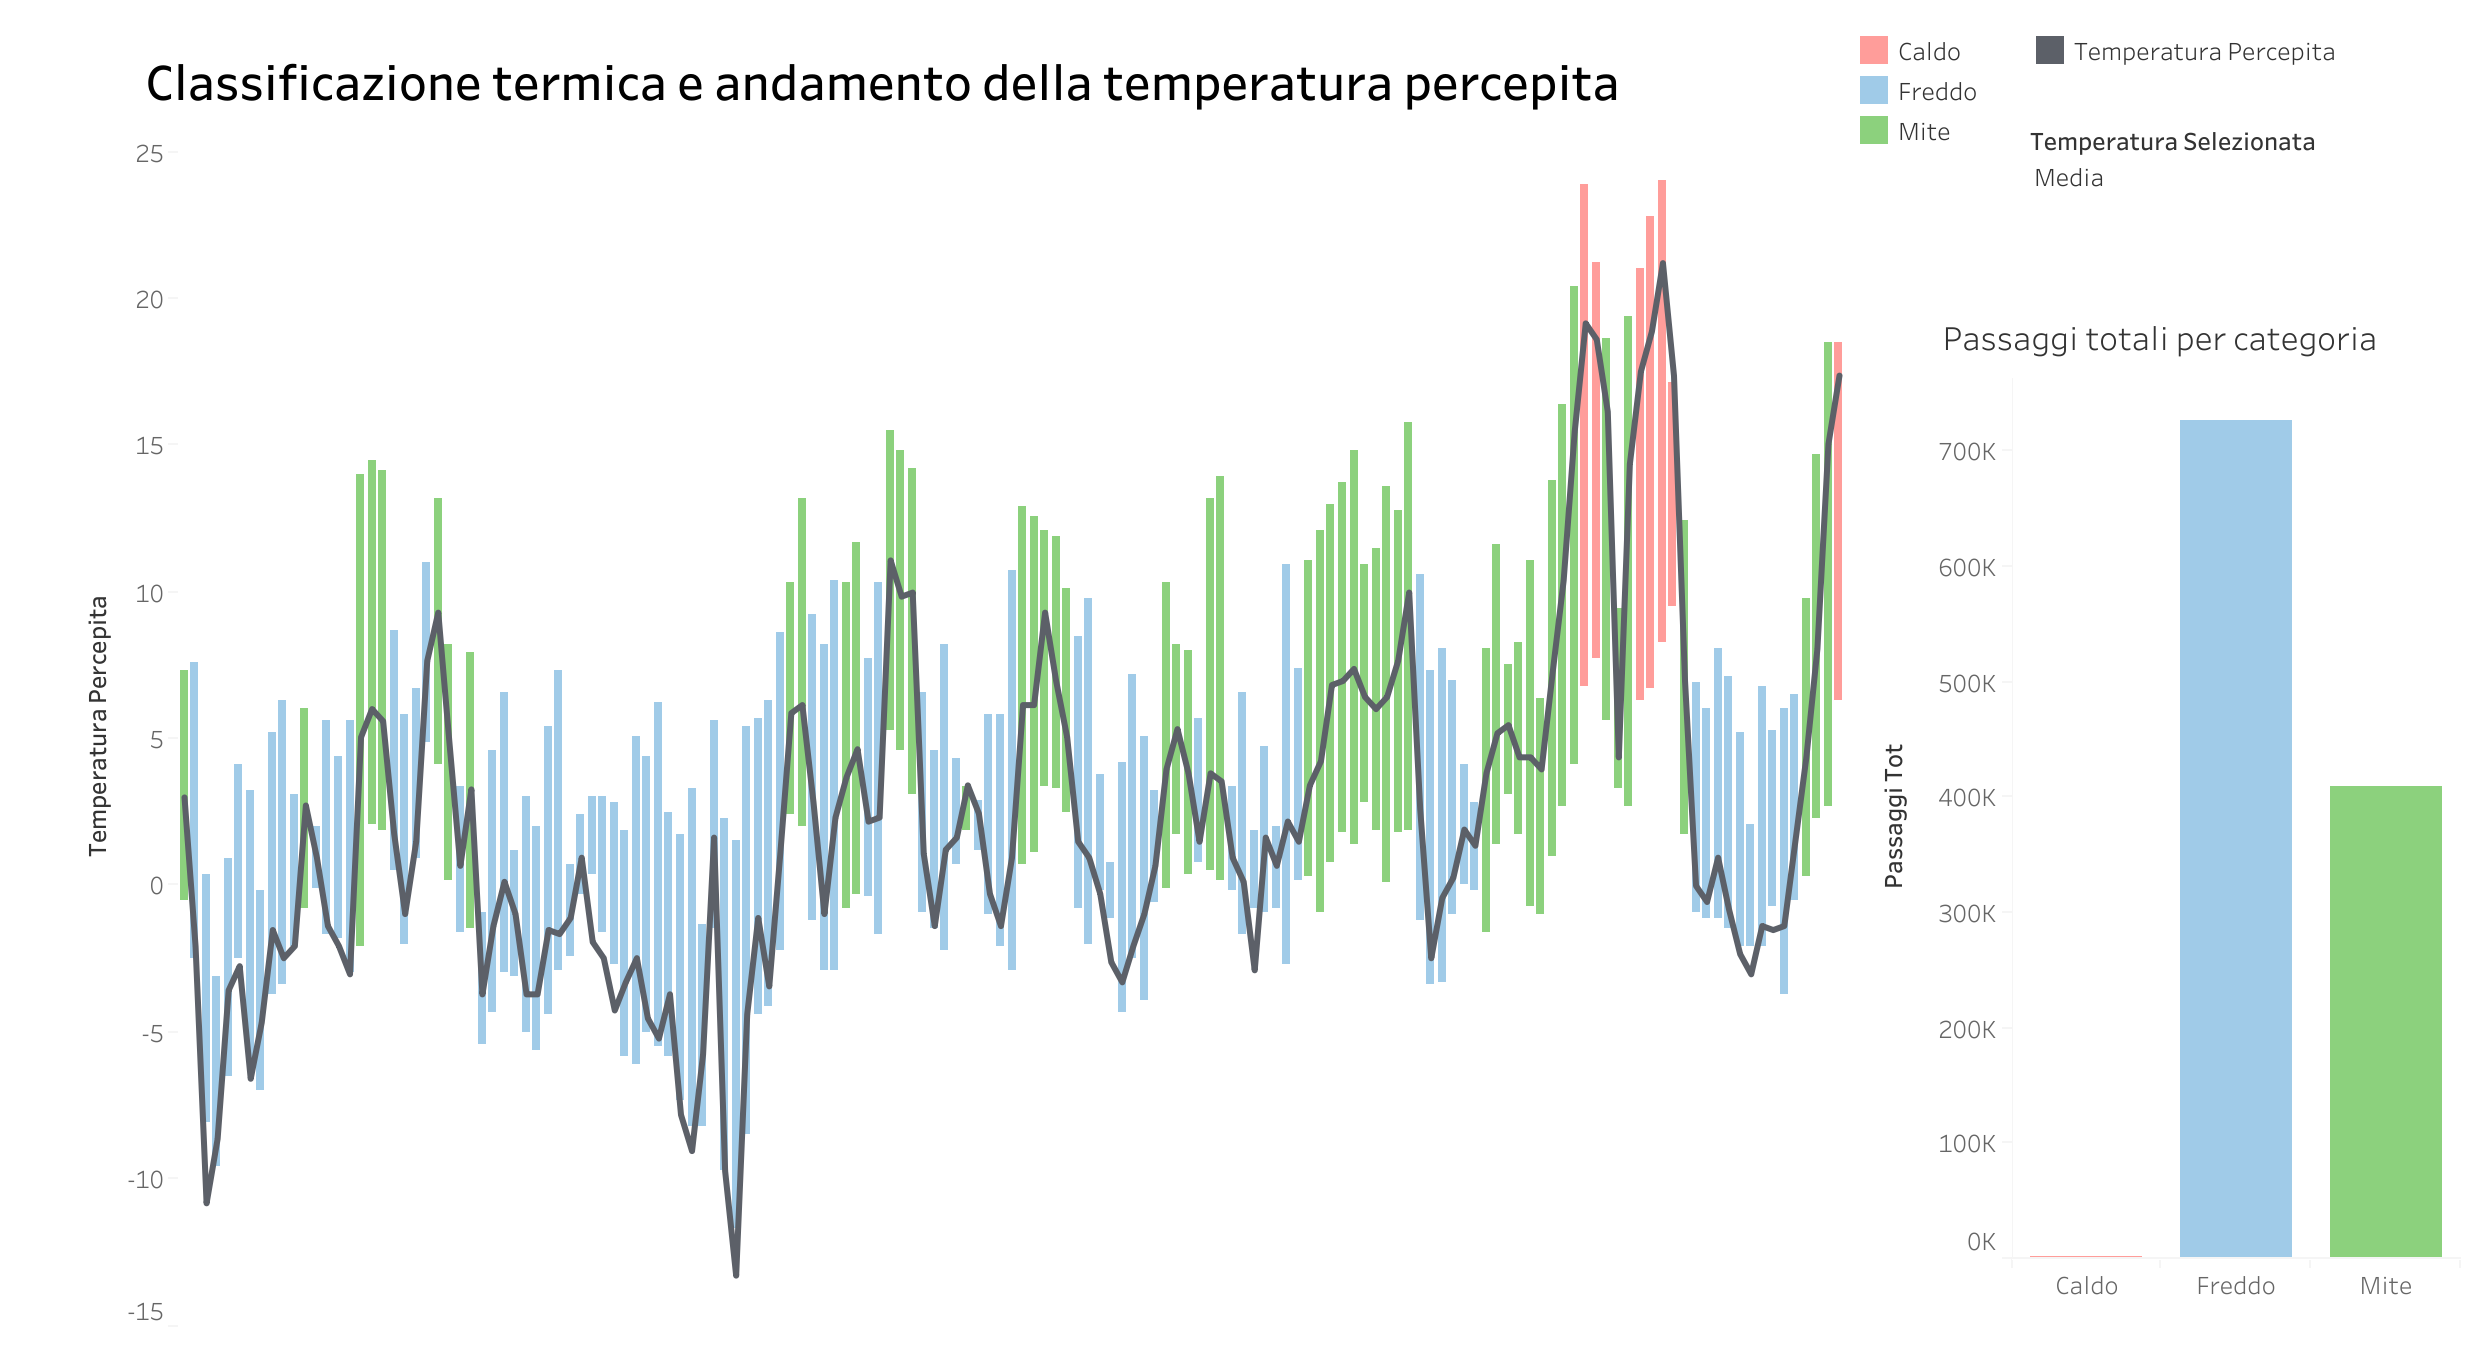
\includegraphics[width=0.95\textwidth]{images/Tableau/Studio_3/Classificazione Termica.png}
    \caption{Dashboard di classificazione termica e andamento della temperatura percepita}
    \label{fig:Classificazione termica}
\end{figure}



\paragraph{Struttura della visualizzazione e variabili impiegate}
\begin{itemize}
    \item \textbf{Asse X}: nella vista principale l’asse delle ascisse rappresenta le \textbf{date} dell’intera stagione, consentendo di associare ogni valore al relativo giorno di rilevazione. Nella vista secondaria, invece, l’asse X riporta le \textbf{categorie di temperatura} (\textit{freddo}, \textit{mite}, \textit{caldo}).
    
    \item \textbf{Asse Y}: nella vista principale viene impiegato un \textbf{doppio asse}. Il primo visualizza la \textbf{temperatura minima} e il parametro \textbf{Range Size}, che genera le barre verticali sospese e rappresenta l’escursione termica giornaliera. Il secondo asse mostra la \textbf{temperatura percepita}, rappresentata da una linea grigia sovrapposta alle barre.
    
    \item \textbf{Filtri e colorazioni}: ogni categoria termica è associata a un colore distinto (freddo = blu, mite = verde, caldo = rosso), mentre la linea della temperatura percepita è grigia per garantire contrasto e leggibilità. È inoltre presente un \textbf{parametro interattivo} che consente di modificare la base di calcolo della temperatura, scegliendo tra temperatura media (impostazione predefinita) e temperatura minima (vedi Appendice~\ref{appendix:Temp_Base}).
    
    \item \textbf{Tipologia di grafico}: combinazione a \textbf{doppio asse} costituita da barre verticali e linea continua, integrata da una vista secondaria a barre semplici per la distribuzione dei passaggi totali per categoria di temperatura.
\end{itemize}


\paragraph{Valutazioni e osservazioni}

Questa dashboard consente di catalogare e analizzare tutte le giornate della stagione, fornendo una rappresentazione continua delle variazioni termiche e delle condizioni percepite.  
Osservata in combinazione con le altre visualizzazioni, permette di collocare ciascun giorno all’interno di una specifica categoria termica e di interpretarne il potenziale impatto sui flussi di affluenza.\\

Dall’andamento della temperatura percepita si osservano diversi picchi minimi particolarmente bassi, in alcuni casi accentuati dall’effetto del vento.  
La vista secondaria evidenzia come le giornate fredde non costituiscano un deterrente per la pratica sciistica: rappresentano infatti la quota maggiore di presenza, quasi il doppio rispetto ai giorni classificati come “miti”.  
Al contrario, le giornate “calde” risultano estremamente limitate, appena sette in tutta la stagione, concentrate nella fase finale.\\

Verso la conclusione della stagione si nota inoltre un progressivo aumento dell’escursione termica giornaliera. Questo fenomeno, pur non potendo essere direttamente correlato ai flussi orari di affluenza (non inclusi in questo studio), suggerisce una possibile influenza sulla qualità della neve nelle ore centrali della giornata, che tende a deteriorarsi più rapidamente rispetto alle prime ore del mattino.


%-----------------------------------------

\section{Analisi 4 – Impatto delle giornate nevose sulle tipologie di Skipass}
\label{sec:analisi4}

La quarta analisi integra i dati meteorologici  personalizzati forniti da \textbf{ARPA Veneto}, relativi alle giornate caratterizzate da precipitazioni nevose, con i dati sui passaggi ai tornelli suddivisi per tipologia di Skipass.  
L’obiettivo  è comprendere in che misura le condizioni meteorologiche, e in particolare la presenza di neve, incidano sull’affluenza agli impianti e sull’utilizzo delle diverse tipologie di titolo di accesso.
La dashboard realizzata presenta una vista principale e due viste di supporto interattive, tra loro collegate attraverso parametri e filtri comuni.\\

Nella \textbf{vista principale} viene mostrato l’andamento giornaliero dei passaggi ai tornelli durante l’intera stagione invernale. Le colonne corrispondenti alle giornate di neve sono evidenziate con una colorazione distinta, in modo da rendere immediatamente visibile la distribuzione e l’intensità dei passaggi in relazione agli eventi nevosi.  
Questa rappresentazione consente di individuare rapidamente se, e in che misura, le giornate con precipitazioni abbiano determinato variazioni significative nei flussi di utenza rispetto alle giornate senza neve.\\

Le \textbf{viste secondarie}, collocate nella parte destra della dashboard, forniscono una sintesi numerica e comparativa dell’analisi.  
La prima riporta il totale complessivo dei passaggi avvenuti in giornate con e senza neve, mentre la seconda mostra la media giornaliera dei passaggi nelle stesse condizioni.  
Queste visualizzazioni complementari offrono una lettura aggregata del fenomeno e risultano utili per verificare la coerenza e l'ampiezza dell'impatto meteorologico osservato nel grafico principale.\\


Tutti i grafici sono collegati dai filtri che consentono di selezionare la condizione meteorologica (assenza o presenza di neve), e dal selettore di tipologia skipass (DS, Valle o Totale), nell'immagine è selezionato il titolo \textbf{DS} (vedi appendice \ref{fig:Impatto_neve_Valle} per altra vista).
La modifica di un parametro determina quindi l'aggiornamento di tutte le viste. Le due viste di supporto sono inoltre connesse a un filtro di mensilità per mostrare totali e medie anche in relazione ai vari mesi della stagione.
Tale filtro non è applicato alla vista principale, poiché l'obiettivo di quest'ultima è evidenziare la distribuzione complessiva delle giornate nevose lungo l'intero arco stagionale.
Di seguito viene presentata la visualizzazione completa nella figura ~\ref{fig:Impatto_neve}.

\newpage


\begin{figure}[htbp]
    \centering
    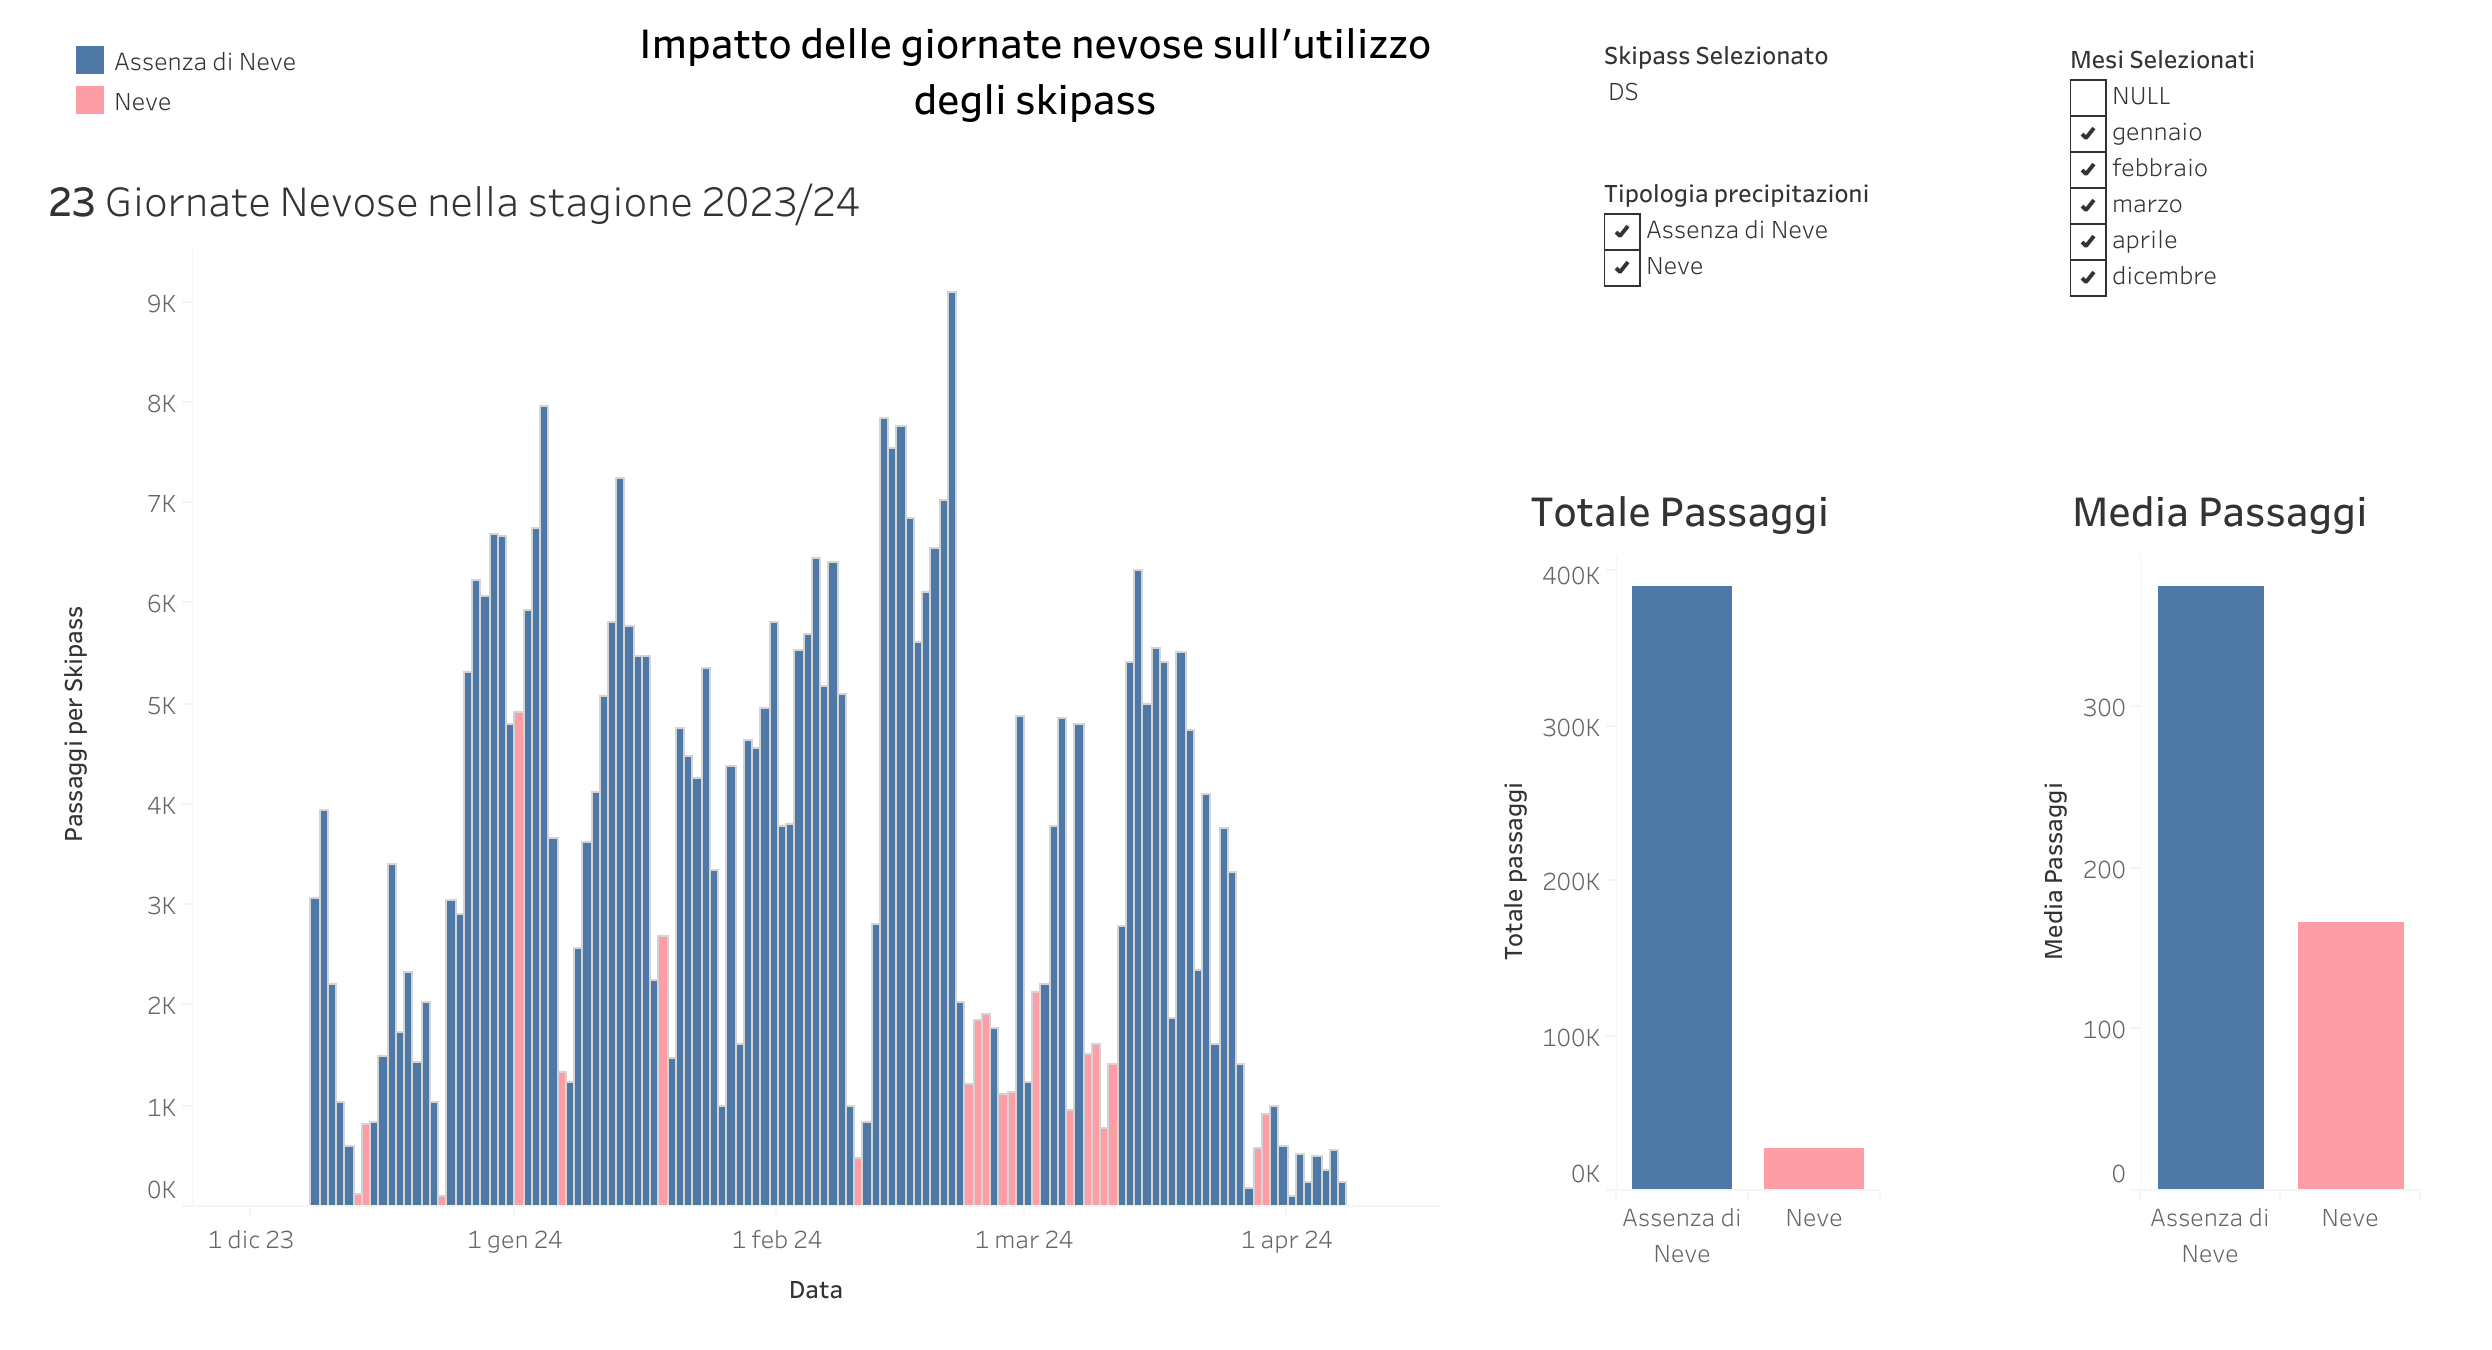
\includegraphics[width=0.95\textwidth]{images/Tableau/Studio_4/Impatto Neve.png}
    \caption{Dashboard Impatto giornate sull'utilizzo degli Skipass, vista Dolomiti Superski}
    \label{fig:Impatto_neve}
\end{figure}

\paragraph{Struttura della visualizzazione e variabili Impiegate}
\begin{itemize}
    \item \textbf{Asse X}: per la vista principale rappresenta la data (misura Continua); per le viste secondarie è invece impiegato il parametro \textbf{Neve} che distingue le date caratterizzate da una precipitazione nevosa (valore Neve), da quelle senza precipitazioni (valore Assenza di Neve)\footnote{Basato sui dati personalizzati forniti da ARPA \cite{ARPAV_private}.}.
    \item \textbf{Asse Y}: nella vista principale riporta il numero di passaggi in funzione della tipologia di skipass selezionata; nelle viste secondarie utilizza il medesimo parametro all’interno delle funzioni di aggregazione \textbf{Somma} e \textbf{Media}, rispettivamente per rappresentare i valori totali e medi giornalieri.
    \item \textbf{Filtri e colorazioni}: le colorazioni differenziano visivamente le giornate con neve (rosa) da quelle senza neve (blu); l’utente può scegliere se visualizzare entrambe o solo una delle due categorie. È inoltre presente un filtro a scelta singola per la tipologia di skipass basato sul parametro "Selezione Skipass" e, nelle viste secondarie, un filtro a scelta multipla che consente di selezionare i mesi da visualizzare.
    \item \textbf{Tipologia di grafico}: grafici a barre multiple, impiegate per entrambe le visualizzazioni.
\end{itemize}

\paragraph{Valutazioni e osservazioni}

Dall’analisi della vista principale e dei valori aggregati e medi giornalieri emerge che le giornate caratterizzate da precipitazioni nevose comportano una riduzione significativa dei passaggi complessivi agli impianti per entrambe le tipologie di skipass.
Tuttavia, l’intensità dell’impatto varia in modo sensibile: gli utenti dotati di \textbf{skipass Dolomiti Superski} registrano, nelle giornate con neve, un’affluenza pari a circa il \textbf{44\%} di quella osservata nelle giornate senza precipitazioni, mentre per gli utenti con \textbf{skipass Valle} tale valore si attesta intorno al \textbf{52\%} (Tabella~\ref{tab:Neve_medie}).

\begin{table}[h]
    \centering
    \begin{tabular}{lccc}
        \toprule
        \textbf{Tipo Skipass} & \textbf{Media Senza Neve} & \textbf{Media con Neve} & \textbf{Rapporto Neve/Assenza} \\
        \midrule
        Valle & 504,9 & 260,4 & 51,6\% \\
        DS & 374,4 & 165,9 & 44,3\% \\
        \bottomrule
    \end{tabular}
    \caption{\textbf{Medie giornaliere} di passaggi con e senza precipitazioni nevose, suddivise per tipologia di Skipass.}
    \label{tab:Neve_medie}
\end{table}


Questo andamento, in cui il titolo “DS” mostra una flessione più marcata rispetto al titolo “Valle”, è confermato anche dal confronto dei \textbf{passaggi totali}: il rapporto tra giornate con e senza precipitazioni nevose risulta infatti leggermente inferiore per lo skipass Dolomiti Superski (Tabella~\ref{tab:Neve_totali}), confermando una maggiore sensibilità di questa categoria di utenza alle condizioni meteorologiche.

\begin{table}[h]
    \centering
    \begin{tabular}{lccc}
        \toprule
        \textbf{Tipo Skipass} & \textbf{Passaggi Senza Neve} & \textbf{Passaggi con Neve} & \textbf{Rapporto Neve/Assenza} \\
        \midrule
        Valle & 526.056 & 43.232 & 8,2\% \\
        DS & 390.099 & 27.539 & 7,1\% \\
        \bottomrule
    \end{tabular}
    \caption{\textbf{Passaggi totali} con e senza precipitazioni nevose, suddivisi per tipologia di Skipass.}
    \label{tab:Neve_totali}
\end{table}


Questa differenza suggerisce che la presenza di neve influenzi in misura maggiore i flussi di sciatori  detentori di skipass DS, spesso non locali o provenienti da altri comprensori, verosimilmente a causa delle difficoltà di spostamento o delle peggiori condizioni di visibilità.
Al contrario, gli utenti titolari di \textbf{skipass Valle}mostrano un comportamento più stabile, confermando una maggiore propensione a frequentare gli impianti anche in condizioni meteorologiche avverse.
Tale tendenza potrebbe inoltre essere ricondotta alla diversa modalità di utilizzo dei titoli di accesso: gli sciatori in possesso di \textbf{skipass Dolomiti Superski} tendono più spesso a disporre di abbonamenti stagionali, che consentono una maggiore flessibilità nella scelta delle giornate di sci, mentre chi acquista uno \textbf{skipass Valle} spesso lo fa per periodi più brevi, ed è quindi generalmente più incline a sfruttare appieno il proprio acquisto, anche in presenza di condizioni meteo meno favorevoli.\\

In sintesi, la neve rappresenta un fattore limitante per l’affluenza complessiva, ma il suo effetto è modulato dalla tipologia di utenza e dal tipo di titolo di accesso utilizzato.\footnote{\textbf{Nota:} Per una vista complessiva delle 4 dashboard principali presentate in questo capitolo si veda l'appendice nella figura \ref{fig:vista_completa}.
Inoltre l'intero materiale è disponibile sul sito di Tableau Public visitabile inquadrando il QR code presente nella figura \ref{fig:qr_tableau} all'interno dell'appendice}


%-----------------------------------------

    
    % Conclusions
    
\chapter{Risultati e Conclusioni}
\label{cha:Conclusioni}

Il presente capitolo riassume i principali risultati emersi dall’analisi multidimensionale condotta sui dati di affluenza agli impianti sciistici gestiti da \textbf{Freccia nel Cielo}, integrati con i dati meteorologici forniti da \textbf{ARPA Veneto}.  
Le analisi, realizzate mediante lo strumento di data visualization \textit{Tableau}, hanno permesso di indagare le dinamiche stagionali, settimanali e meteorologiche che influenzano la presenza degli utenti sulle piste, evidenziando pattern ricorrenti e tendenze specifiche del contesto di Cortina d’Ampezzo.

\section{Sintesi dei risultati delle analisi}


\subsection*{Picchi stagionali di affluenza}
Dall’analisi~\ref{sec:analisi1} emerge che il periodo natalizio rappresenta il picco massimo di affluenza agli impianti, come prevedibile in relazione ai flussi turistici stagionali.  
Tuttavia, lo stesso periodo si caratterizza anche per una forte variabilità giornaliera: pur registrando i valori più elevati della stagione, mostra un andamento irregolare, con oscillazioni marcate tra giornate di alta e bassa affluenza, come evidenziato nel grafico dei passaggi totali nella figura~\ref{fig:passaggi_tot_stagione}.\\

Lo studio ha inoltre evidenziato come il periodo di \textbf{Carnevale} presenti un comportamento opposto: non raggiunge i picchi assoluti del Natale, ma mostra una notevole \textbf{stabilità} dei flussi, con una media di passaggi giornalieri elevata e costante sia durante le festività sia nei giorni immediatamente successivi.  
In sostanza, il periodo più equilibrato e regolare, con affluenze elevate ma meno soggette a variazioni improvvise, risulta essere proprio quello carnevalesco, come confermato anche dal grafico dei passaggi totali con esclusione del periodo natalizio (figura~\ref{fig:passaggi_tot_noNatale}). \\

Si può quindi concludere che, sebbene il turismo invernale sia fortemente trainato dal periodo natalizio, anche il Carnevale riveste un ruolo significativo nel sostenere i livelli di affluenza complessiva.

\subsection*{Variazioni settimanali e pattern giornalieri}
L’analisi~\ref{sec:analisi2}, articolata nelle sue due viste principali, ha evidenziato due tendenze particolarmente interessanti e, in parte, inattese.  
In primo luogo, il \textbf{sabato} risulta essere la giornata settimanale con la maggiore affluenza complessiva, superando la \textbf{domenica}, che comunemente è considerata la giornata più frequentata sulle piste.  
Questo andamento si conferma in modo costante per l’intera stagione, come mostrato nella vista superiore della figura~\ref{fig:Weekend_cumulativo}, dove la linea viola, corrispondente al sabato, risulta quasi sempre la più alta rispetto a quella rossa della domenica.\\

Un secondo risultato significativo emerge considerando l’intera settimana: analizzando il grafico inferiore, che rappresenta la \textbf{somma cumulativa dei passaggi} per giorno, si osserva che il secondo giorno per volume complessivo non appartiene al weekend, bensì è il \textbf{martedì}.  
Questo comportamento, visualizzabile nella dashboard con l’inclusione del martedì (figura~\ref{fig:dash_tuesday} in appendice), risulta inaspettato ma coerente con la presenza di flussi turistici prolungati o nuovi arrivi settimanali.\\

Queste evidenze offrono indicazioni pratiche di rilievo per la \textbf{gestione operativa} e la pianificazione delle risorse negli impianti della valle, suggerendo la necessità di un’attenzione particolare non solo ai weekend, ma anche ai giorni centrali della settimana, potenzialmente interessanti per attività promozionali o iniziative di fidelizzazione.


\subsection*{Classificazione e influenza delle condizioni meteorologiche}
L’analisi~\ref{sec:analisi3} ha permesso di classificare tutte le giornate della stagione in tre categorie termiche — \textbf{freddo}, \textbf{mite} e \textbf{caldo} — grazie all’utilizzo di campi calcolati che considerano non solo la temperatura rilevata, ma anche l’effetto del vento sulla temperatura percepita sulle piste.  
Questa classificazione consente di ottenere una rappresentazione più realistica delle condizioni ambientali vissute dagli sciatori, fornendo una base solida per correlare le variabili meteorologiche con i livelli di affluenza.\\

Combinata con le altre analisi del capitolo, questa dashboard rappresenta uno strumento utile per interpretare l’impatto meteorologico delle singole giornate, permettendo di individuare rapidamente le situazioni potenzialmente più favorevoli o critiche in termini di presenze.  
Nella vista principale, illustrata in figura~\ref{fig:Classificazione termica}, ogni giorno è rappresentato da una barra colorata in funzione della categoria termica, mentre la linea sovrapposta mostra l’andamento della temperatura percepita nel corso della stagione.  
Si osserva come, nella seconda metà dell’inverno, la tendenza generale sia verso un progressivo aumento dell’escursione termica giornaliera, visibile dall’ampliarsi delle barre verticali: questo fenomeno suggerisce un maggiore sbalzo tra le ore mattutine e quelle pomeridiane, con possibili implicazioni sulla qualità della neve e sulle abitudini di presenza sulle piste.  
È infatti plausibile che tali condizioni inducano gli sciatori a preferire le prime ore del giorno, quando la neve mantiene caratteristiche migliori.\\

La vista secondaria della dashboard evidenzia invece la \textbf{distribuzione dei passaggi totali} per categoria termica.  
Da questa si nota come le giornate fredde non rappresentino un deterrente per la pratica sciistica: al contrario, registrano il \textbf{maggior volume di passaggi}, quasi più del doppio rispetto alle giornate miti.  
Le giornate calde, al contrario, risultano estremamente limitate, solo sette in tutta la stagione, e il numero di passaggi in tali condizioni risulta trascurabile rispetto alle altre due categorie. \\ 

Nel complesso, l’analisi conferma che gli sciatori tendono ad adattarsi bene alle basse temperature, mentre i fattori che richiederebbero un ulteriore analisi con l'aiuto di parametri orari sono quelli dell'escursione termica.
Queste informazioni offrono un importante contributo per la comprensione del comportamento degli utenti e per la pianificazione di attività o servizi in base alle condizioni meteorologiche prevalenti.


\subsection*{Impatto delle giornate nevose e differenze tra tipologie di Skipass}
L’analisi~\ref{sec:analisi4} ha approfondito l’effetto delle giornate caratterizzate da precipitazioni nevose sull’affluenza complessiva e, in particolare, sulle due principali tipologie di skipass in uso: \textbf{Valle} (per cui si veda la vista in appendice \ref{fig:Impatto_neve_Valle}) e \textbf{Dolomiti Superski (DS)}.  
L’obiettivo era valutare se e in che misura la presenza di neve, generalmente considerata un elemento favorevole all’attività sciistica, potesse invece incidere negativamente sulla partecipazione quotidiana, influenzando in modo differenziato i diversi segmenti di utenza.\\

L’impatto sulle presenze totali è evidente: come mostrato nella figura~\ref{fig:Impatto_neve}, le colonne rosa, corrispondenti alle giornate con precipitazioni nevose, si associano quasi sempre a livelli di affluenza inferiori rispetto alle giornate senza neve.  
Solo in rari casi, in coincidenza con periodi di particolare richiamo turistico, si osservano valori comparabili.  
Questo comportamento suggerisce che, sebbene la neve costituisca un fattore essenziale per l’attività sciistica nel lungo periodo, le giornate in cui essa cade effettivamente rappresentano un ostacolo momentaneo per l’affluenza, probabilmente anche a causa della scarsa visibilità o delle condizioni di trasporto e spostamento.\\

L’effetto sui diversi tipi di skipass emerge con chiarezza dalle viste secondarie della dashboard, che riportano i valori di \textbf{passaggi medi} e \textbf{passaggi totali} nelle giornate con e senza precipitazioni.  
Dalle tabelle~\ref{tab:Neve_medie} e~\ref{tab:Neve_totali} risulta che la riduzione più marcata si registra per lo skipass \textbf{Dolomiti Superski}, la cui media giornaliera di passaggi nelle giornate nevose è pari al \textbf{44,3\%} di quella osservata in assenza di neve, contro il \textbf{51,6\%} rilevato per lo skipass \textbf{Valle}.  
La stessa tendenza, seppur in misura più contenuta, si conferma anche nei passaggi totali: rispettivamente \textbf{7,1\%} per lo skipass DS e \textbf{8,2\%} per quello Valle.  
Questi dati, pur evidenziando differenze numericamente ridotte, sono statisticamente significativi per comprendere il diverso comportamento dei due segmenti di utenza e, di fatto, dei due titoli.\\

Il comportamento differenziale osservato può essere attribuito alla diversa composizione e abitudine d’uso dei due gruppi di sciatori.  
Gli utenti dotati di skipass \textbf{Dolomiti Superski}, spesso non locali o provenienti da altri comprensori, risultano più sensibili alle condizioni meteorologiche e logistiche, rinunciando più facilmente alla giornata di sci in presenza di neve o maltempo.  
Al contrario, gli sciatori titolari di skipass \textbf{Valle}, in gran parte utenti locali o abituali, mostrano una maggiore costanza di partecipazione anche in condizioni meteo avverse.  
Questo risultato può essere spiegato anche dalla diversa tipologia di abbonamento: gli skipass stagionali, più diffusi tra gli utenti DS, offrono una maggiore flessibilità nella scelta dei giorni di utilizzo e non impongono la necessità di “sfruttare” ogni giornata disponibile.  
Gli skipass di breve durata, tipici invece della categoria Valle, incentivano un utilizzo più continuo, anche in presenza di precipitazioni, poiché l’utente tende a voler valorizzare al massimo il proprio acquisto.\\
Nel complesso, l’analisi dimostra come la neve, pur essendo elemento simbolicamente positivo per il contesto sciistico, rappresenti un fattore \textbf{limitante nel breve periodo}, che riduce la frequenza delle visite giornaliere.  
Tuttavia, l’impatto non è uniforme e risulta modulato dalla tipologia di skipass, dal profilo dell’utenza e dalle motivazioni di accesso.  
Queste evidenze possono supportare strategie di comunicazione e pricing mirate, ad esempio promozioni nei giorni nevosi o incentivi per l’utenza turistica, con l’obiettivo di attenuare le flessioni di affluenza legate alle condizioni atmosferiche.


\section{Riflessioni finali e sviluppi futuri}

I risultati ottenuti mostrano come l’integrazione tra dati operativi e meteorologici consenta di costruire strumenti analitici efficaci per il \textbf{supporto decisionale} nella gestione degli impianti sciistici.  
La possibilità di visualizzare in modo interattivo i diversi scenari stagionali e meteorologici permette di anticipare i picchi di domanda, ottimizzare la distribuzione delle risorse e migliorare la pianificazione del personale.  
L’uso combinato di tecniche di \textit{data visualization} e di un modello a costellazione dei dati ha inoltre dimostrato la capacità di rappresentare in maniera chiara e sintetica fenomeni complessi, rendendo accessibili anche a figure non tecniche informazioni strategiche per la gestione quotidiana e per la programmazione stagionale.

In prospettiva, l’ampliamento del dataset a più aree scisitche  e l’inclusione di nuove variabili, come l’origine geografica dei visitatori, la tipologia di impianto o i dati orari di accesso,  potrebbero arricchire ulteriormente l’analisi, consentendo di modellare con maggiore precisione la relazione tra condizioni ambientali, caratteristiche del pubblico e comportamento dell’utenza.  

In sintesi, il lavoro svolto dimostra come un approccio basato sulla \textbf{Business Intelligence territoriale} e sulla \textbf{data visualization} possa fornire un contributo concreto alla gestione operativa utile e consapevole delle destinazioni turistiche alpine, promuovendo un utilizzo più efficiente delle risorse, una migliore esperienza per i visitatori e un'organizzazioe più strutturata favorevole ai lavoratori. \\ 

Infine, si sottolinea che la metodologia e l’impostazione analitica sviluppate in questo elaborato sono pienamente \textbf{replicabili e adattabili} ad altri comprensori sciistici o località turistiche montane.  
Applicando lo stesso modello di integrazione tra dati operativi e informazioni meteorologiche — opportunamente personalizzato con i dati locali di ciascuna realtà — è possibile ottenere risultati analoghi, capaci di generare \textbf{indicatori specifici e comparabili} tra diverse aree.  
Questo rende il modello proposto uno strumento flessibile e scalabile, utile non solo per singole aziende impiantistiche, ma anche per enti di promozione turistica o amministrazioni locali che desiderino comprendere e ottimizzare le dinamiche di affluenza legate alle condizioni ambientali e stagionali.




    % Ringraziamenti
    \cleardoublepage
\thispagestyle{empty}

\vspace*{2cm}

\begin{center}
{\Huge \textbf{Ringraziamenti}}
\end{center}

\vspace{2cm}

\begin{flushleft}

Innanzitutto desidero ringraziare il mio relatore, il Professor Paolo Bouquet, per il supporto, la disponibilità, e le indicazioni che hanno permesso e guidato lo sviluppo di questo elaborato.
\par\vspace{2em}

Un ringraziamento speciale va ad ARPA Veneto e a Tofana srl - Freccia nel Cielo, enti che hanno reso possibile questo lavoro fornendo i dati e il supporto necessari allo sviluppo della ricerca. Desidero esprimere la mia sincera gratitudine a tutto il personale coinvolto per la disponibilità e la collaborazione dimostrata.
\par\vspace{2em}

In particolare, ringrazio Alessandra Biasin per la grande disponibilità,  l’assistenza e i consigli forniti durante la ricerca delle informazioni e la stesura di questo elaborato.
\par\vspace{2em}

Ringrazio di cuore i miei genitori, Mamma e Papà, per avermi sempre sostenuto e incoraggiato in ogni passo del mio percorso.
Li ringrazio soprattutto per avermi reso libero e responsabile delle mie scelte, come quella di intraprendere questa strada, e per aver riposto sempre fiducia nel mio giudizio, nelle decisioni giuste come in quelle meno fortunate.
\par\vspace{2em}

Ringrazio tutte le persone che, a Trento, mi hanno accompagnato in questo viaggio universitario. \\
Un ringraziamento speciale va a Filippo, il mio coinquilino, con cui ho condiviso innumerevoli cene e altrettante sconfitte a Mario Kart; a Michela, con cui ho condiviso viaggi in macchina, ravioli e un’infinità di ore in aula studio, sempre terminate dalle nostre meritate pause GT; e a Stefano, con cui ho condiviso l’intero percorso, tra casa e università. Sei stato una costante motivazione per me, un aiuto prezioso quando i miei programmi sembravano non compilare neanche, e ho sempre apprezzato i nostri ripassoni notturni pre-esame dopo aver ordinato a domicilio.
\par\vspace{2em}

Infine, ringrazio tutti i miei amici, che mi hanno supportato e sopportato mentre cercavo di spiegare, spesso fallendo, cosa stessi studiando in quel momento. Grazie, e scusate. \\ 
Un ringraziamento speciale va a Sandro e Lorenzo, che mi hanno accompagnato, e continuano a farlo, in ogni fase del mio percorso, universitario e non, sia a distanza che a casa.
Mi avete sempre motivato a dare il meglio di me, e continuate tutt’ora a farlo. Spero di riuscire a restituirvi almeno una parte di ciò che mi date ogni giorno.
Grazie per credere sempre in me: per me siete come una famiglia.
\par\vspace{2em}

\end{flushleft}

\cleardoublepage


  \endgroup

  % Bibliography
  \addcontentsline{toc}{chapter}{Bibliografia}
  % Alphabetical order of authors
  \bibliographystyle{unsrt}
  \bibliography{bibliography.bib}

  % Attachments
  \titleformat{\chapter} {\normalfont\Huge\bfseries}{\thechapter}{1em}{}
  \appendix
  \chapter{Appendice}
\label{cha:appendix}

\section*{Codice SQL per la creazione del database}
\label{appendix:sql}

Il seguente codice SQL definisce la struttura del database a \textbf{costellazione}, illustrata nel Capitolo~\ref{cha:Data_op}.  
Sono incluse la creazione delle tabelle dimensionali e dei fatti, le relazioni tra esse e alcuni record di esempio, utili a comprendere la logica di costruzione del modello.

\begin{lstlisting}[language=SQL, caption={Codice SQL di esempio per la creazione del database}]
-- Creazione del database
CREATE DATABASE CortinaAffluenza;
USE CortinaAffluenza;

-- ==========================
-- TABELLE DIMENSIONALI
-- ==========================

CREATE TABLE Dim_Anno (
    Id_Anno  INT AUTO_INCREMENT PRIMARY KEY ,
    Anno INT NOT NULL
);

CREATE TABLE Dim_Mese (
    Id_Mese INT AUTO_INCREMENT PRIMARY KEY ,
    Nome_Mese VARCHAR(20),
    Numero INT,
    Id_Anno INT,
    FOREIGN KEY (Id_Anno) REFERENCES Dim_Anno(Id_Anno)
);

CREATE TABLE Dim_Settimana (
    Id_Settimana INT AUTO_INCREMENT PRIMARY KEY ,
    Id_Mese INT,
    FOREIGN KEY (Id_Mese) REFERENCES Dim_Mese(Id_Mese)
);

CREATE TABLE Dim_Giorno (
    Id_Giorno INT AUTO_INCREMENT PRIMARY KEY ,
    Data DATE,
    Giorno_Sett VARCHAR(15),
    Is_Holiday BOOLEAN,
    Id_Settimana INT,
    FOREIGN KEY (Id_Settimana) REFERENCES Dim_Settimana(Id_Settimana)
);

CREATE TABLE Dim_Temperatura (
    Id_Temperatura INT AUTO_INCREMENT PRIMARY KEY ,
    Temp_Min DECIMAL(5,2),
    Temp_Media DECIMAL(5,2),
    Temp_Max DECIMAL(5,2)
);

CREATE TABLE Dim_Vento (
    Id_Vento INT AUTO_INCREMENT PRIMARY KEY ,
    Direzione VARCHAR(20),
    Velocita DECIMAL(5,2)
);

CREATE TABLE Dim_CondizioneMeteo (
    Id_CondMeteo INT AUTO_INCREMENT PRIMARY KEY ,
    Tipo_Precipitazione DECIMAL(5,2),
    Id_Temperatura INT,
    Id_Vento INT,
    FOREIGN KEY (Id_Temperatura) REFERENCES Dim_Temperatura(Id_Temperatura),
    FOREIGN KEY (Id_Vento) REFERENCES Dim_Vento(Id_Vento)
);

CREATE TABLE Dim_Stagione (
    Id_Stagione INT AUTO_INCREMENT  PRIMARY KEY ,
    Nome_Stagione VARCHAR(30),
    Data_Inizio DATE,
    Data_Fine DATE
);

CREATE TABLE Dim_TipoSkipass (
    Id_Skipass INT AUTO_INCREMENT PRIMARY KEY,
    Nome_Tipologia VARCHAR(30)
);

CREATE TABLE Dim_AreaSciistica (
    Id_Area INT AUTO_INCREMENT PRIMARY KEY,
    Nome_Area VARCHAR(50)
);

CREATE TABLE Dim_Impianto (
    Id_Impianto INT AUTO_INCREMENT PRIMARY KEY ,
    Nome_Impianto VARCHAR(50),
    Tipo_Impianto VARCHAR(30),
    Id_Area INT,
    FOREIGN KEY (Id_Area) REFERENCES Dim_AreaSciistica(Id_Area)
);

-- ==========================
-- TABELLE DEI FATTI
-- ==========================

CREATE TABLE Fatto_AffluenzaGiornaliera (
    Id_Affluenza INT AUTO_INCREMENT PRIMARY KEY ,
    Id_Giorno INT,
    Id_Impianto INT,
    Id_Skipass INT,
    Id_CondMeteo INT,
    Id_Stagione INT,
    Passaggi_Tot INT,
    FOREIGN KEY (Id_Giorno) REFERENCES Dim_Giorno(Id_Giorno),
    FOREIGN KEY (Id_Impianto) REFERENCES Dim_Impianto(Id_Impianto),
    FOREIGN KEY (Id_Skipass) REFERENCES Dim_TipoSkipass(Id_Skipass),
    FOREIGN KEY (Id_CondMeteo) REFERENCES Dim_CondizioneMeteo(Id_CondMeteo),
    FOREIGN KEY (Id_Stagione) REFERENCES Dim_Stagione(Id_Stagione)
);

CREATE TABLE Fatto_AffluenzaStagionale (
    Id_Affluenza_Stagionale INT AUTO_INCREMENT PRIMARY KEY ,
    Id_Impianto INT,
    Id_Skipass INT,
    Id_Stagione INT,
    Passaggi_Totali INT,
    FOREIGN KEY (Id_Impianto) REFERENCES Dim_Impianto(Id_Impianto),
    FOREIGN KEY (Id_Skipass) REFERENCES Dim_TipoSkipass(Id_Skipass),
    FOREIGN KEY (Id_Stagione) REFERENCES Dim_Stagione(Id_Stagione)
);

-- ==========================
-- INSERIMENTO DATI ESEMPLIFICATIVI
-- ==========================

INSERT INTO Dim_Anno (Anno) VALUES (2023), (2024);

INSERT INTO Dim_Mese (Nome_Mese, Numero, Id_Anno)
VALUES ('Gennaio', 1, 1), ('Febbraio', 2, 1);

INSERT INTO Dim_Settimana (Id_Mese) VALUES (1), (2);

INSERT INTO Dim_Giorno (Data, Giorno_Sett, Is_Holiday, Id_Settimana)
VALUES ('2023-01-10', 'Martedi', FALSE, 1),
       ('2023-02-15', 'Mercoledi', FALSE, 2);

INSERT INTO Dim_Temperatura (Temp_Min, Temp_Media, Temp_Max)
VALUES (-10.5, -6.2, -2.1);

INSERT INTO Dim_Vento (Direzione, Velocita)
VALUES ('Nord', 15.3);

INSERT INTO Dim_CondizioneMeteo (Tipo_Precipitazione, Id_Temperatura, Id_Vento)
VALUES (2.0, 1, 1);

INSERT INTO Dim_Stagione (Nome_Stagione, Data_Inizio, Data_Fine)
VALUES ('2023/2024', '2023-12-01', '2024-04-15');

INSERT INTO Dim_TipoSkipass (Nome_Tipologia)
VALUES ('Dolomiti Superski'), ('Di Valle');

INSERT INTO Dim_AreaSciistica (Nome_Area)
VALUES ('Tofana');

INSERT INTO Dim_Impianto (Nome_Impianto, Tipo_Impianto, Id_Area)
VALUES ('Freccia nel Cielo', 'Funivia', 1),
       ('Tofana Express', 'Seggiovia', 1);

INSERT INTO Fatto_AffluenzaGiornaliera
(Id_Giorno, Id_Impianto, Id_Skipass, Id_CondMeteo, Id_Stagione, Passaggi_Tot)
VALUES (1, 1, 1, 1, 1, 1200),
       (2, 2, 2, 1, 1, 850);

INSERT INTO Fatto_AffluenzaStagionale
(Id_Impianto, Id_Skipass, Id_Stagione, Passaggi_Totali)
VALUES (1, 1, 1, 180000),
       (2, 2, 1, 95000);

\end{lstlisting}


\section*{Campi Calcolati}
Di seguito è riportato l’elenco completo dei campi calcolati utilizzati nelle analisi sviluppate su \textit{Tableau}.  
Tali campi hanno permesso di creare variabili dinamiche e derivate, in particolare per il calcolo della temperatura percepita e per la gestione dei parametri meteorologici.

\begin{lstlisting}[language=SQL, caption={Campo calcolato: Temperatura Base}]
IF [TipoTemperatura] = "Minima" THEN
    [Temp Min (C)]
ELSE
    [Temp Media (C)]
END
\end{lstlisting} \label{appendix:Temp_Base}


\begin{lstlisting}[language=SQL, caption={Campo calcolato: Temperatura Percepita (Wind Chill)}]
IF ISNULL([Temperatura Base]) THEN
    NULL
ELSEIF [Temperatura Base] <= 10 
   AND ([Velocita vento  (m/s)] * 3.6) > 4.8 THEN
    ROUND(
        13.12
      + 0.6215 * [Temperatura Base]
      - 11.37 * POWER(([Velocita vento  (m/s)] * 3.6), 0.16)
      + 0.3965 * [Temperatura Base] * POWER(([Velocita vento  (m/s)] * 3.6), 0.16),
    1)
ELSE
    [Temperatura Base]
END
\end{lstlisting}\label{appendix:Temp_percepita}

\begin{lstlisting}[language=SQL, caption={Campo calcolato: Selettore Tipologia di Skipass}]
IF [Selezione Skipass] = "DS" THEN 
    [Pass. DS]

ELSEIF [Selezione Skipass] = "Valle" THEN 
    [Pass. Valle]

ELSE 
    [Passaggi Tot]
END
\end{lstlisting}\label{appendix:tipo_skipass}


\noindent
Nelle sezioni successive sono riportate alcune visualizzazioni supplementari e di dettaglio, non incluse nel corpo principale della tesi ma rilevanti per il completamento dell’analisi.

\section*{Analisi 1}

\subsection*{Specifica Giorno}
Esempio della vista dettagliata di un singolo giorno, che consente di analizzare i valori puntuali dei passaggi registrati nella data selezionata.

\begin{figure}[h]
    \centering
    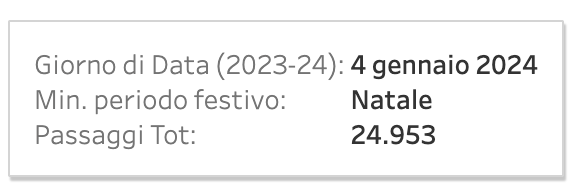
\includegraphics[width=0.5\linewidth]{images/Tableau/Studio_1/4_gennaio.png}
    \caption{Specifica del Giorno}
    \label{fig:spec_giorno}
\end{figure}

\subsection*{Grafico passaggi totali per Settimana}
Versione aggregata del grafico principale dell’analisi 1, ottenuta tramite operazione di \textbf{Roll-Up} sulla gerarchia temporale, che mostra i passaggi totali per settimana.

\begin{figure}[htbp]
    \centering
    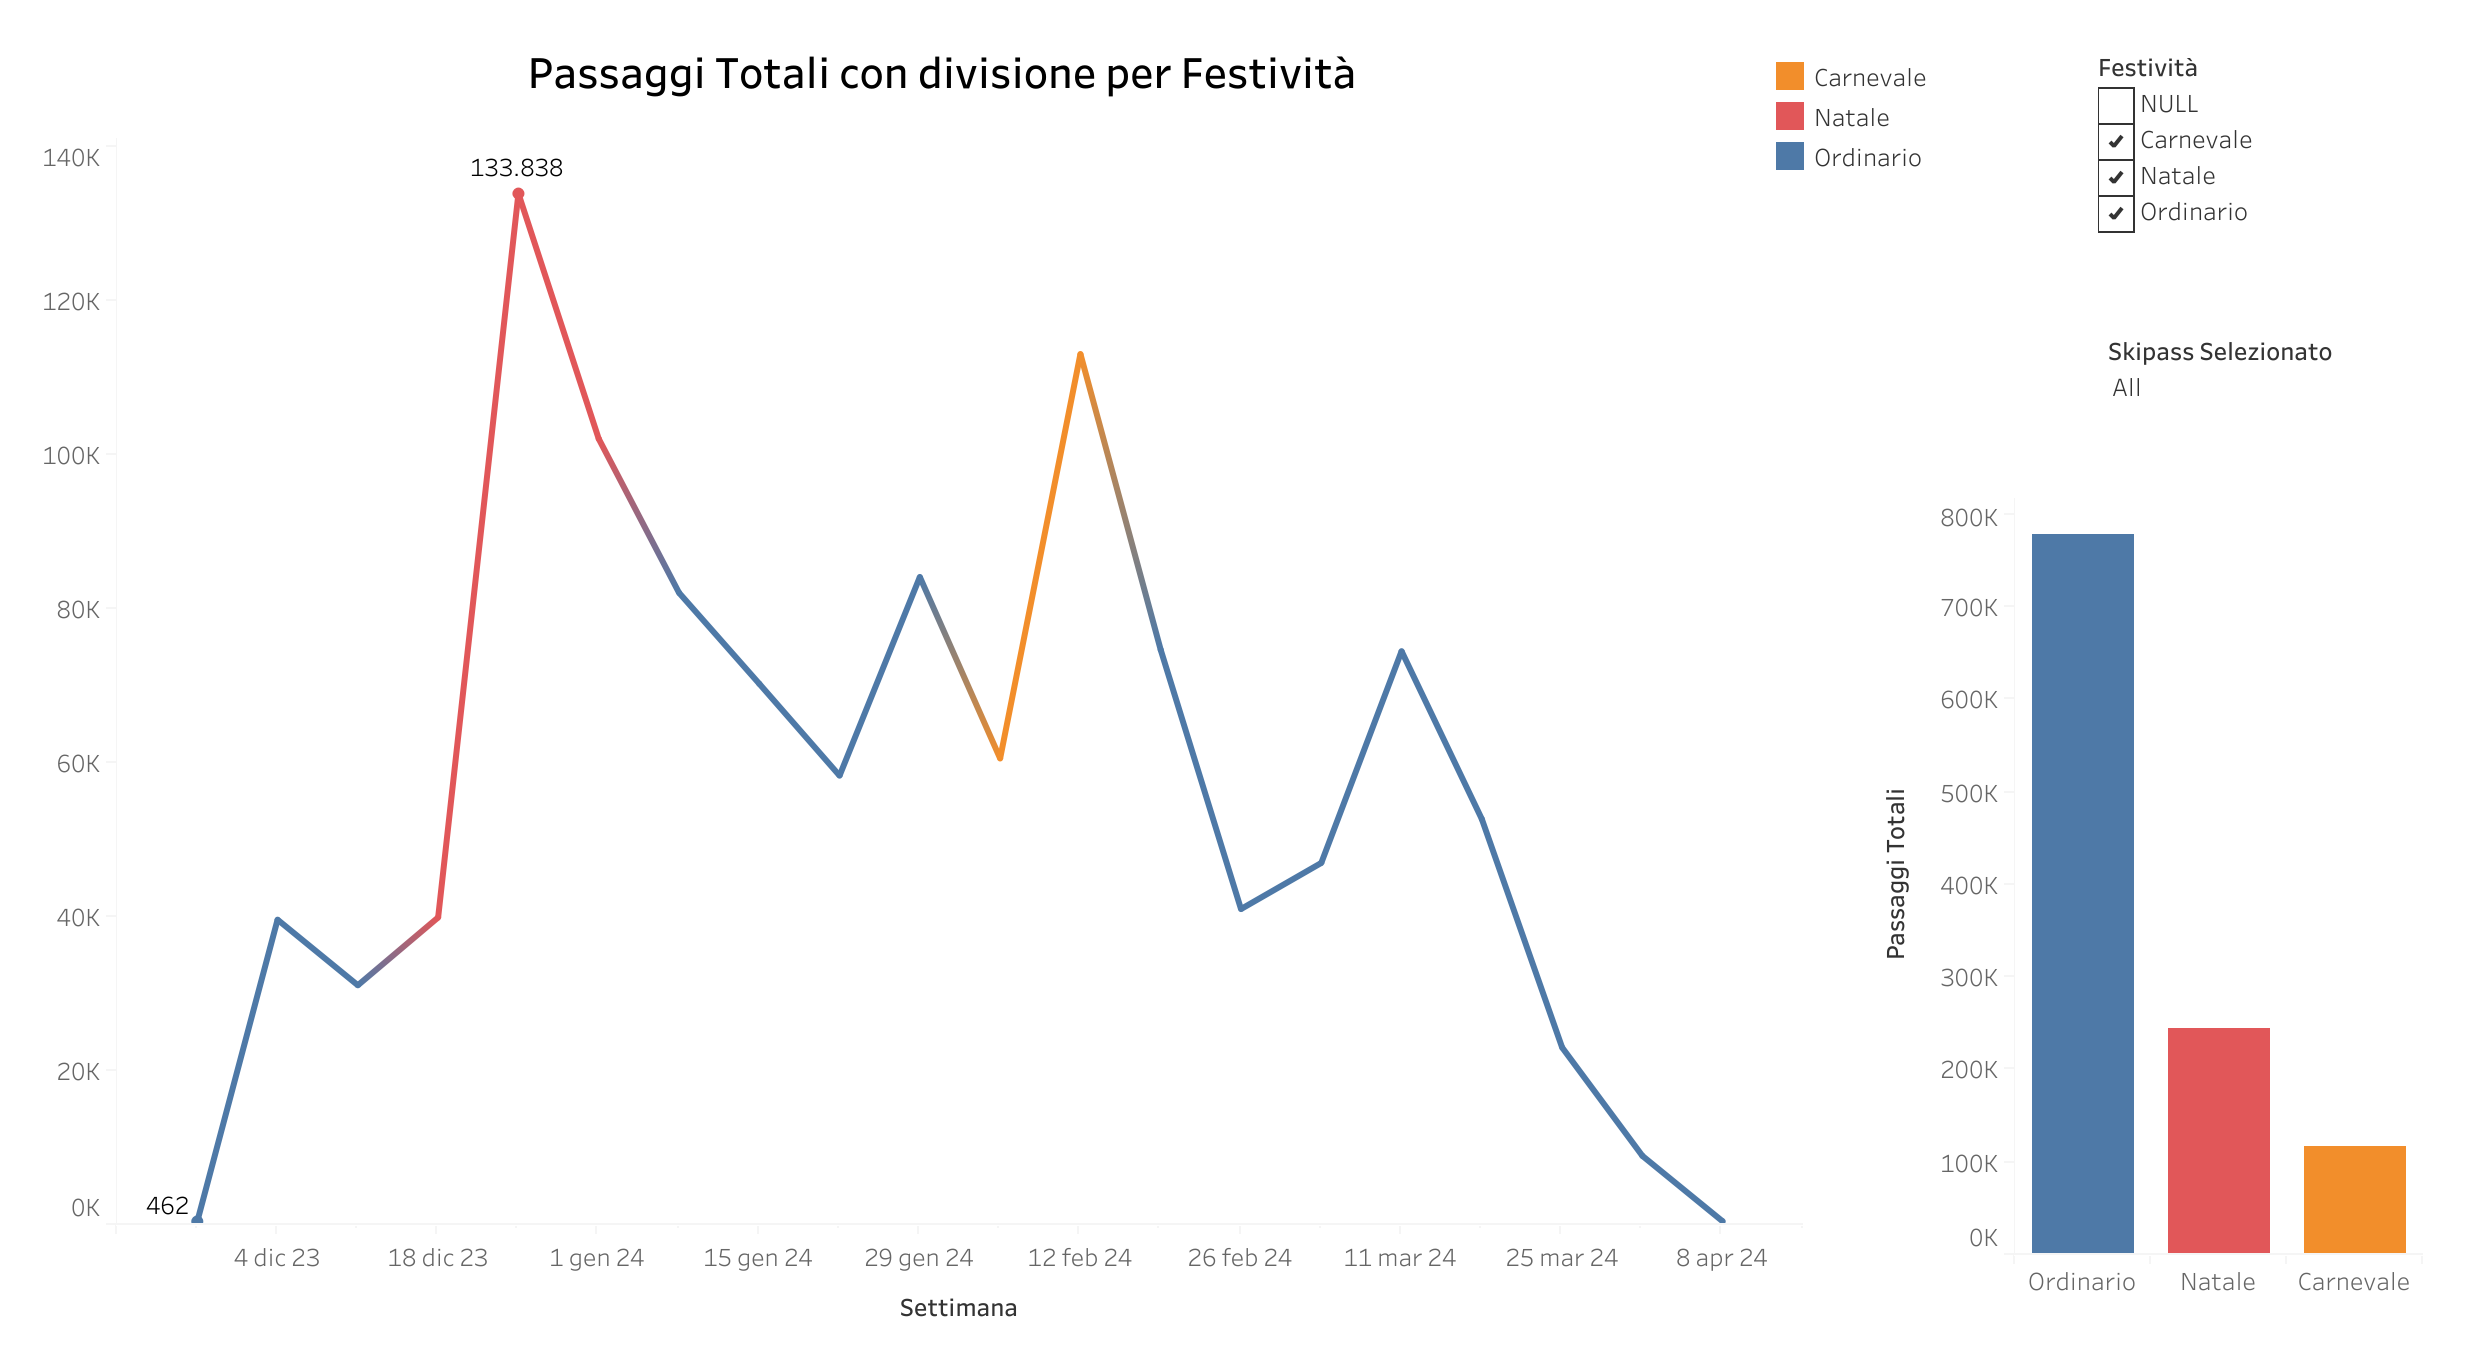
\includegraphics[width=0.95\textwidth]{images/Tableau/Studio_1/Passaggi Totali Settimana.png}
    \caption{Andamento settimanale dei passaggi totali nella stagione 2023–24, suddivisi per periodo festivo.}
    \label{fig:passaggi_tot_settimana}
\end{figure}

\subsection*{Grafico passaggi totali per giorno - Natale}
Vista alternativa del grafico principale della prima analisi, con filtro per l’esclusione del periodo natalizio.  
Questa impostazione evidenzia la costanza del periodo carnevalesco e la sua stabilità nel corso della stagione.

\begin{figure}[htbp]
    \centering
    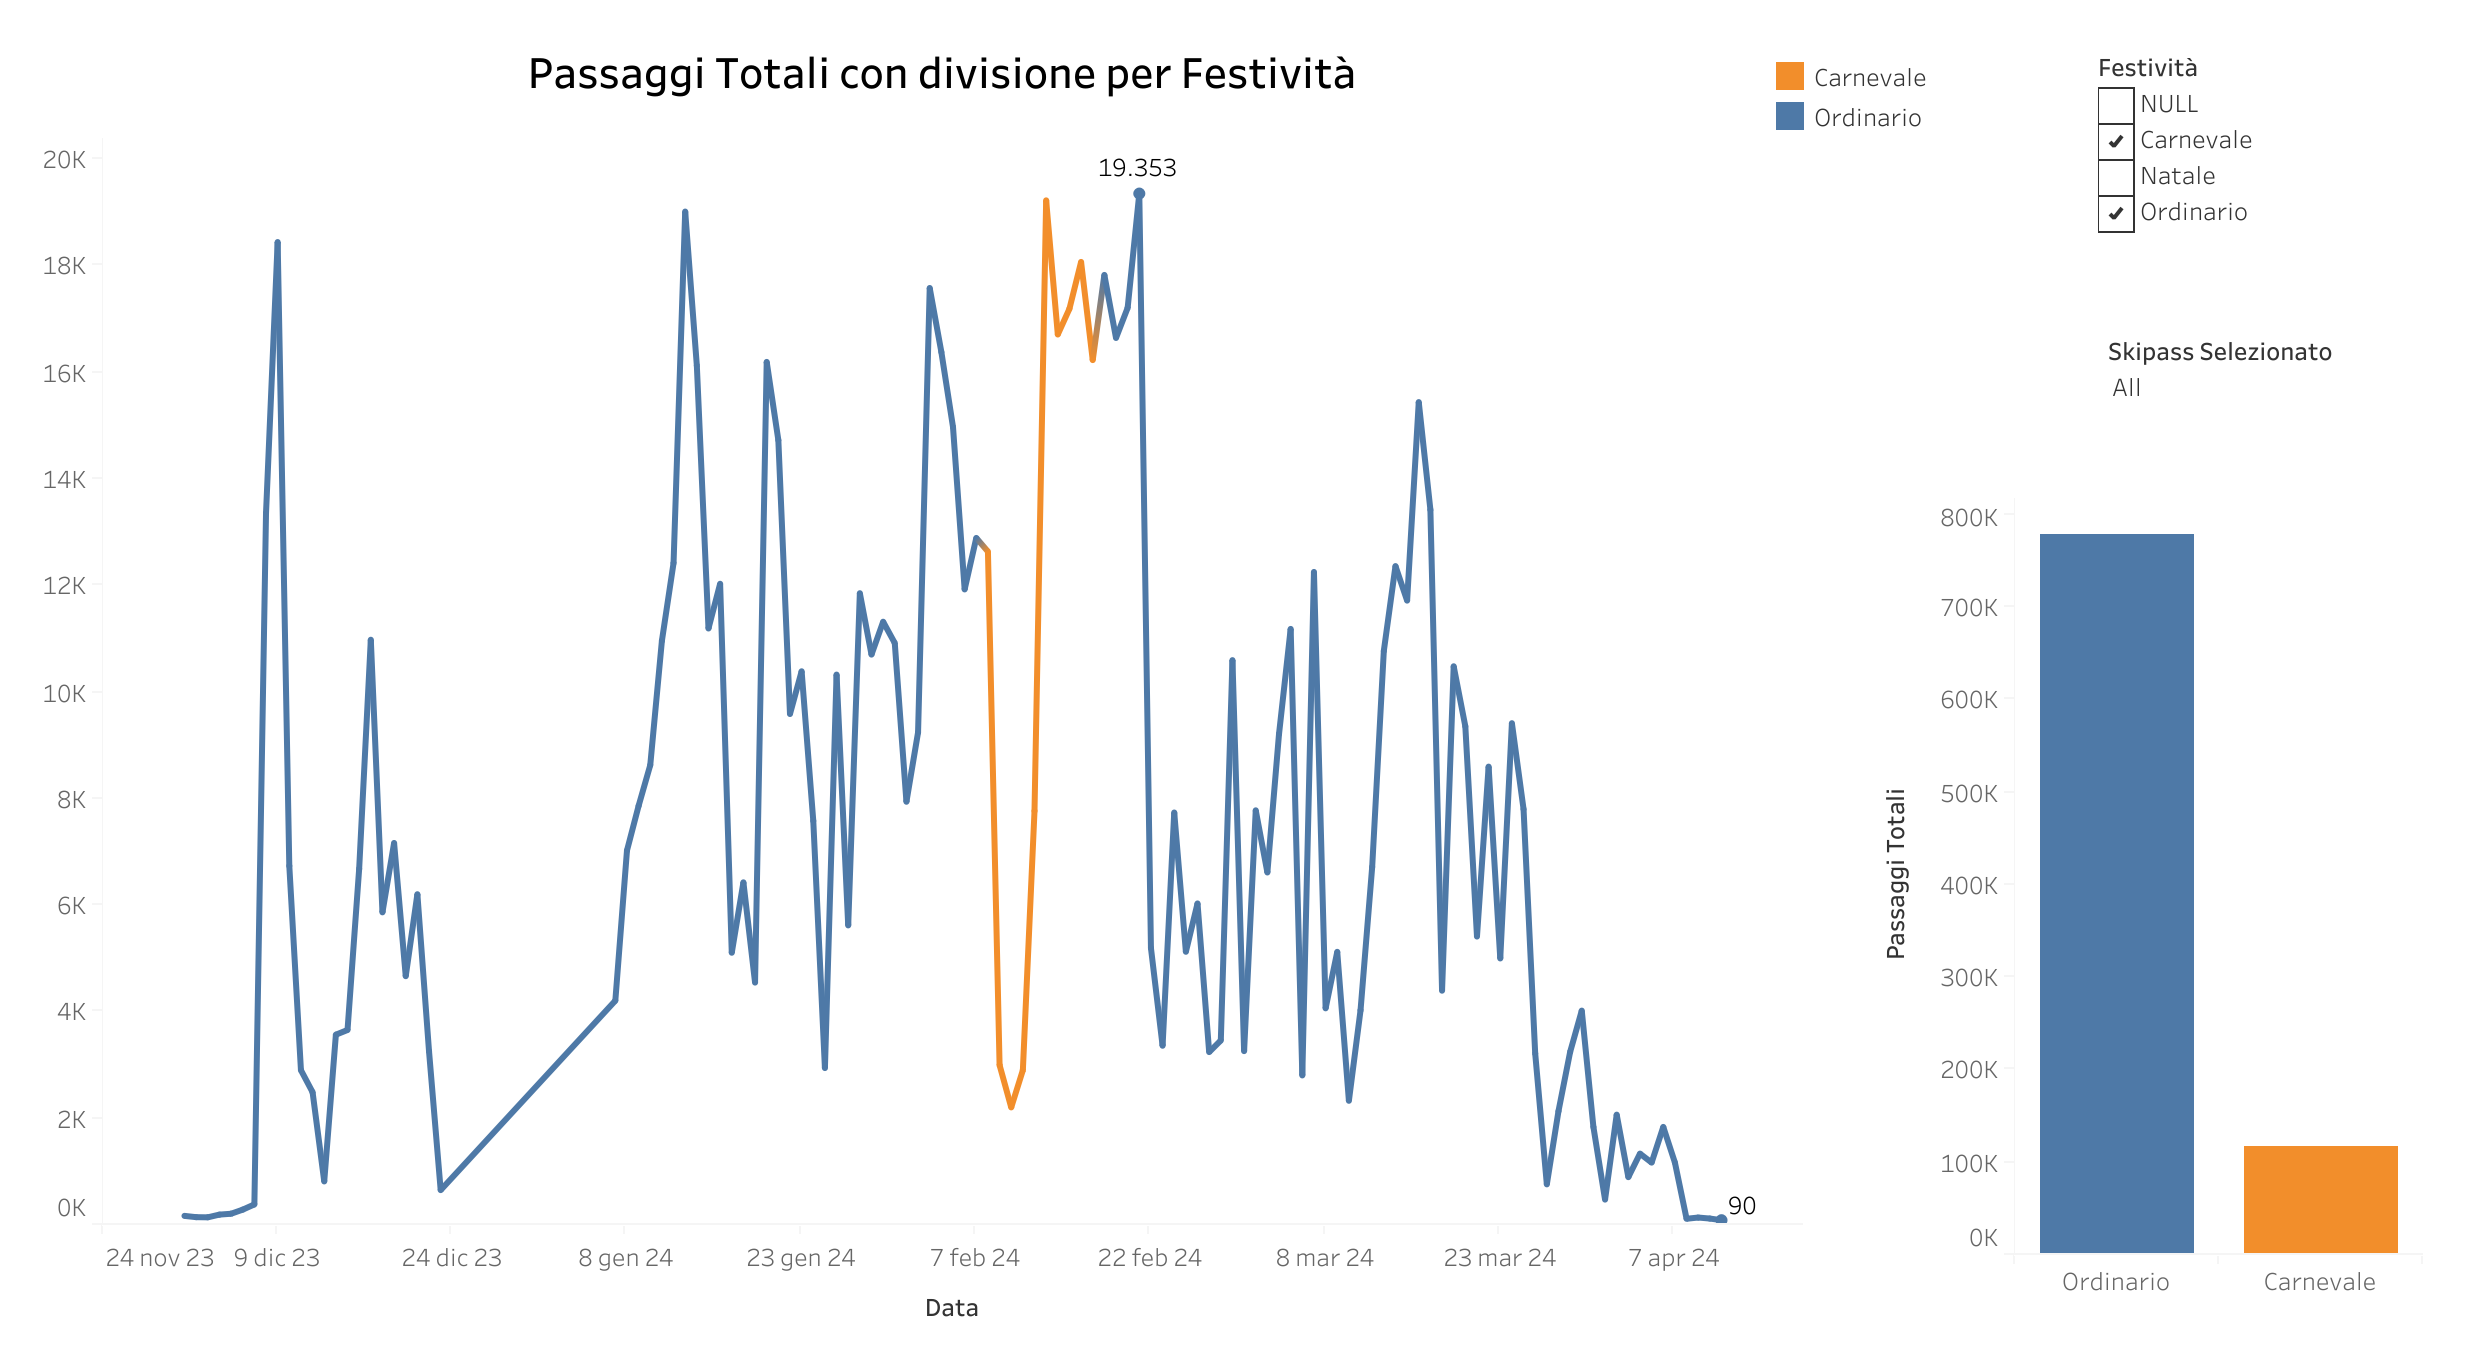
\includegraphics[width=0.9\textwidth]{images/Tableau/Studio_1/Passaggi Totali_noNatale.png}
    \caption{Andamento stagionale dei Passaggi totali con esclusione del periodo Natalizio}
    \label{fig:passaggi_tot_noNatale}
\end{figure}


\section*{Analisi 2}
La seguente dashboard, descritta nel Capitolo~\ref{sec:analisi2}, mostra l’andamento dei passaggi giornalieri per giorno della settimana.  
In questa vista è stato incluso anche il \textbf{martedì} attraverso il filtro “\textbf{Selezione Giorno}”, per evidenziare la sua rilevanza in termini di affluenza.

\begin{figure}[htbp]
    \centering
    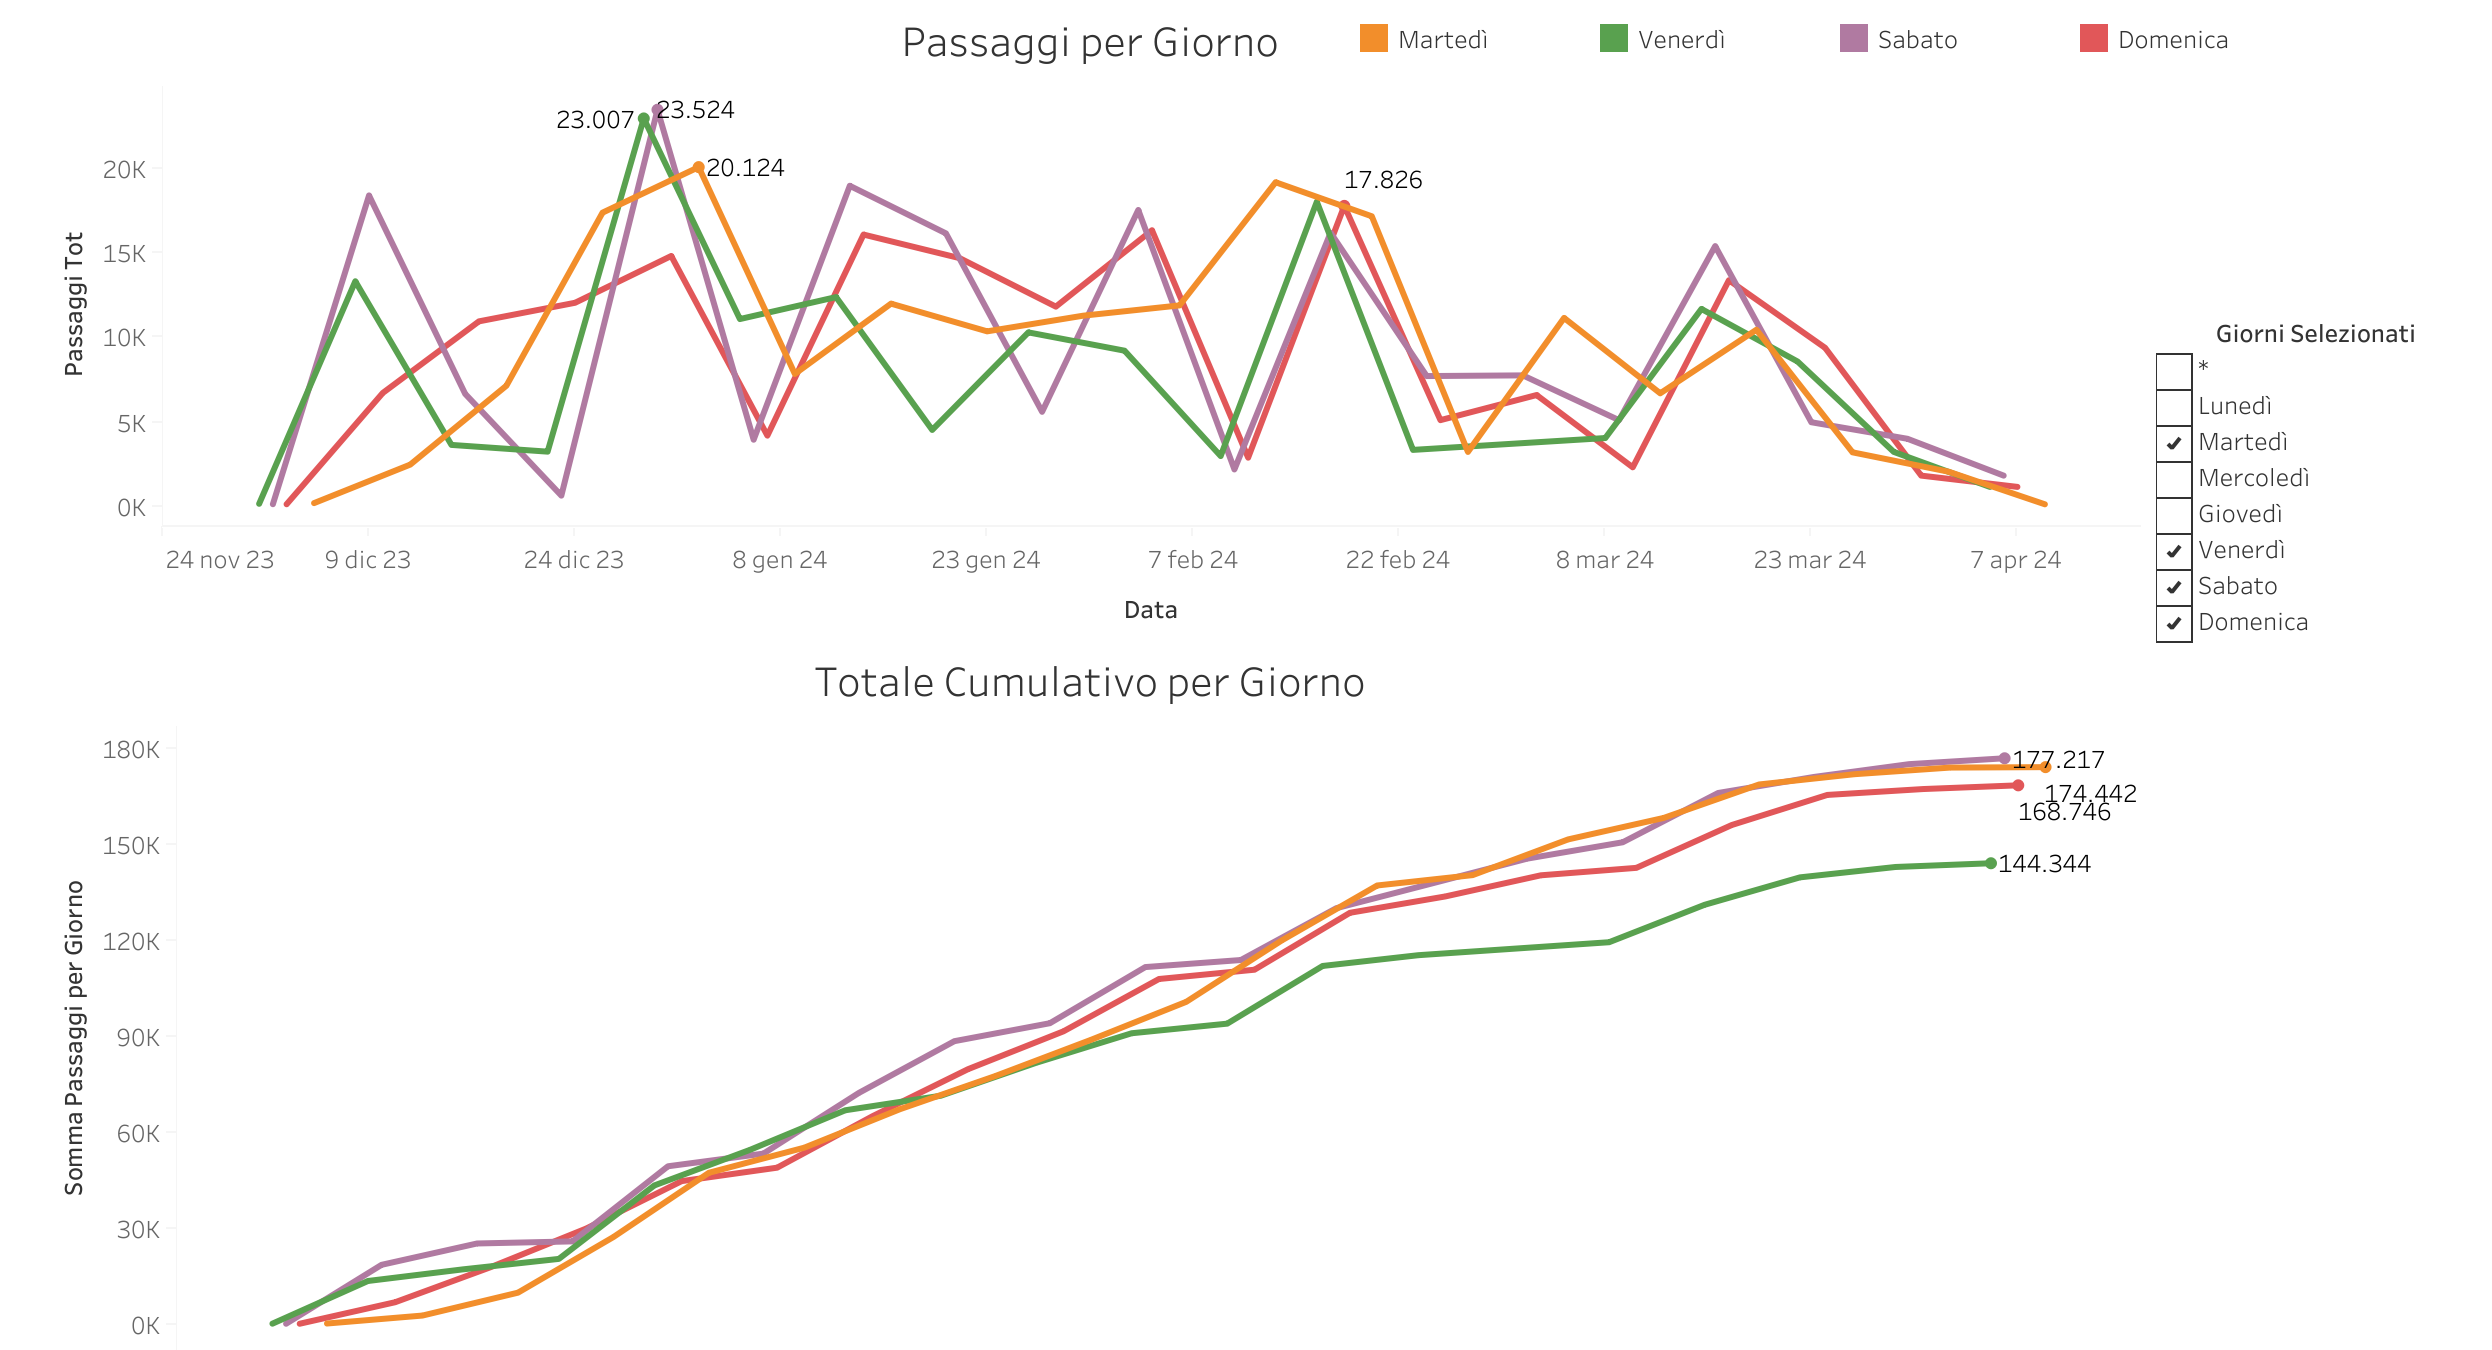
\includegraphics[width=0.9\textwidth]{images/Tableau/Studio_2/Dash_Tuesday.png}
    \caption{Dashboard per passaggi settimanali con totale cumulativo con l'inclusione del Martedì.}
    \label{fig:dash_tuesday}
\end{figure}


\section*{Analisi 4}
Di seguito vengono riportati i campi calcolati e le dashboard utilizzate per l’analisi sull’impatto delle precipitazioni nevose in relazione alle diverse tipologie di skipass.  
La figura seguente mostra l’esempio riferito agli utenti in possesso dello \textbf{skipass di Valle}.




\begin{figure}[htbp]
    \centering
    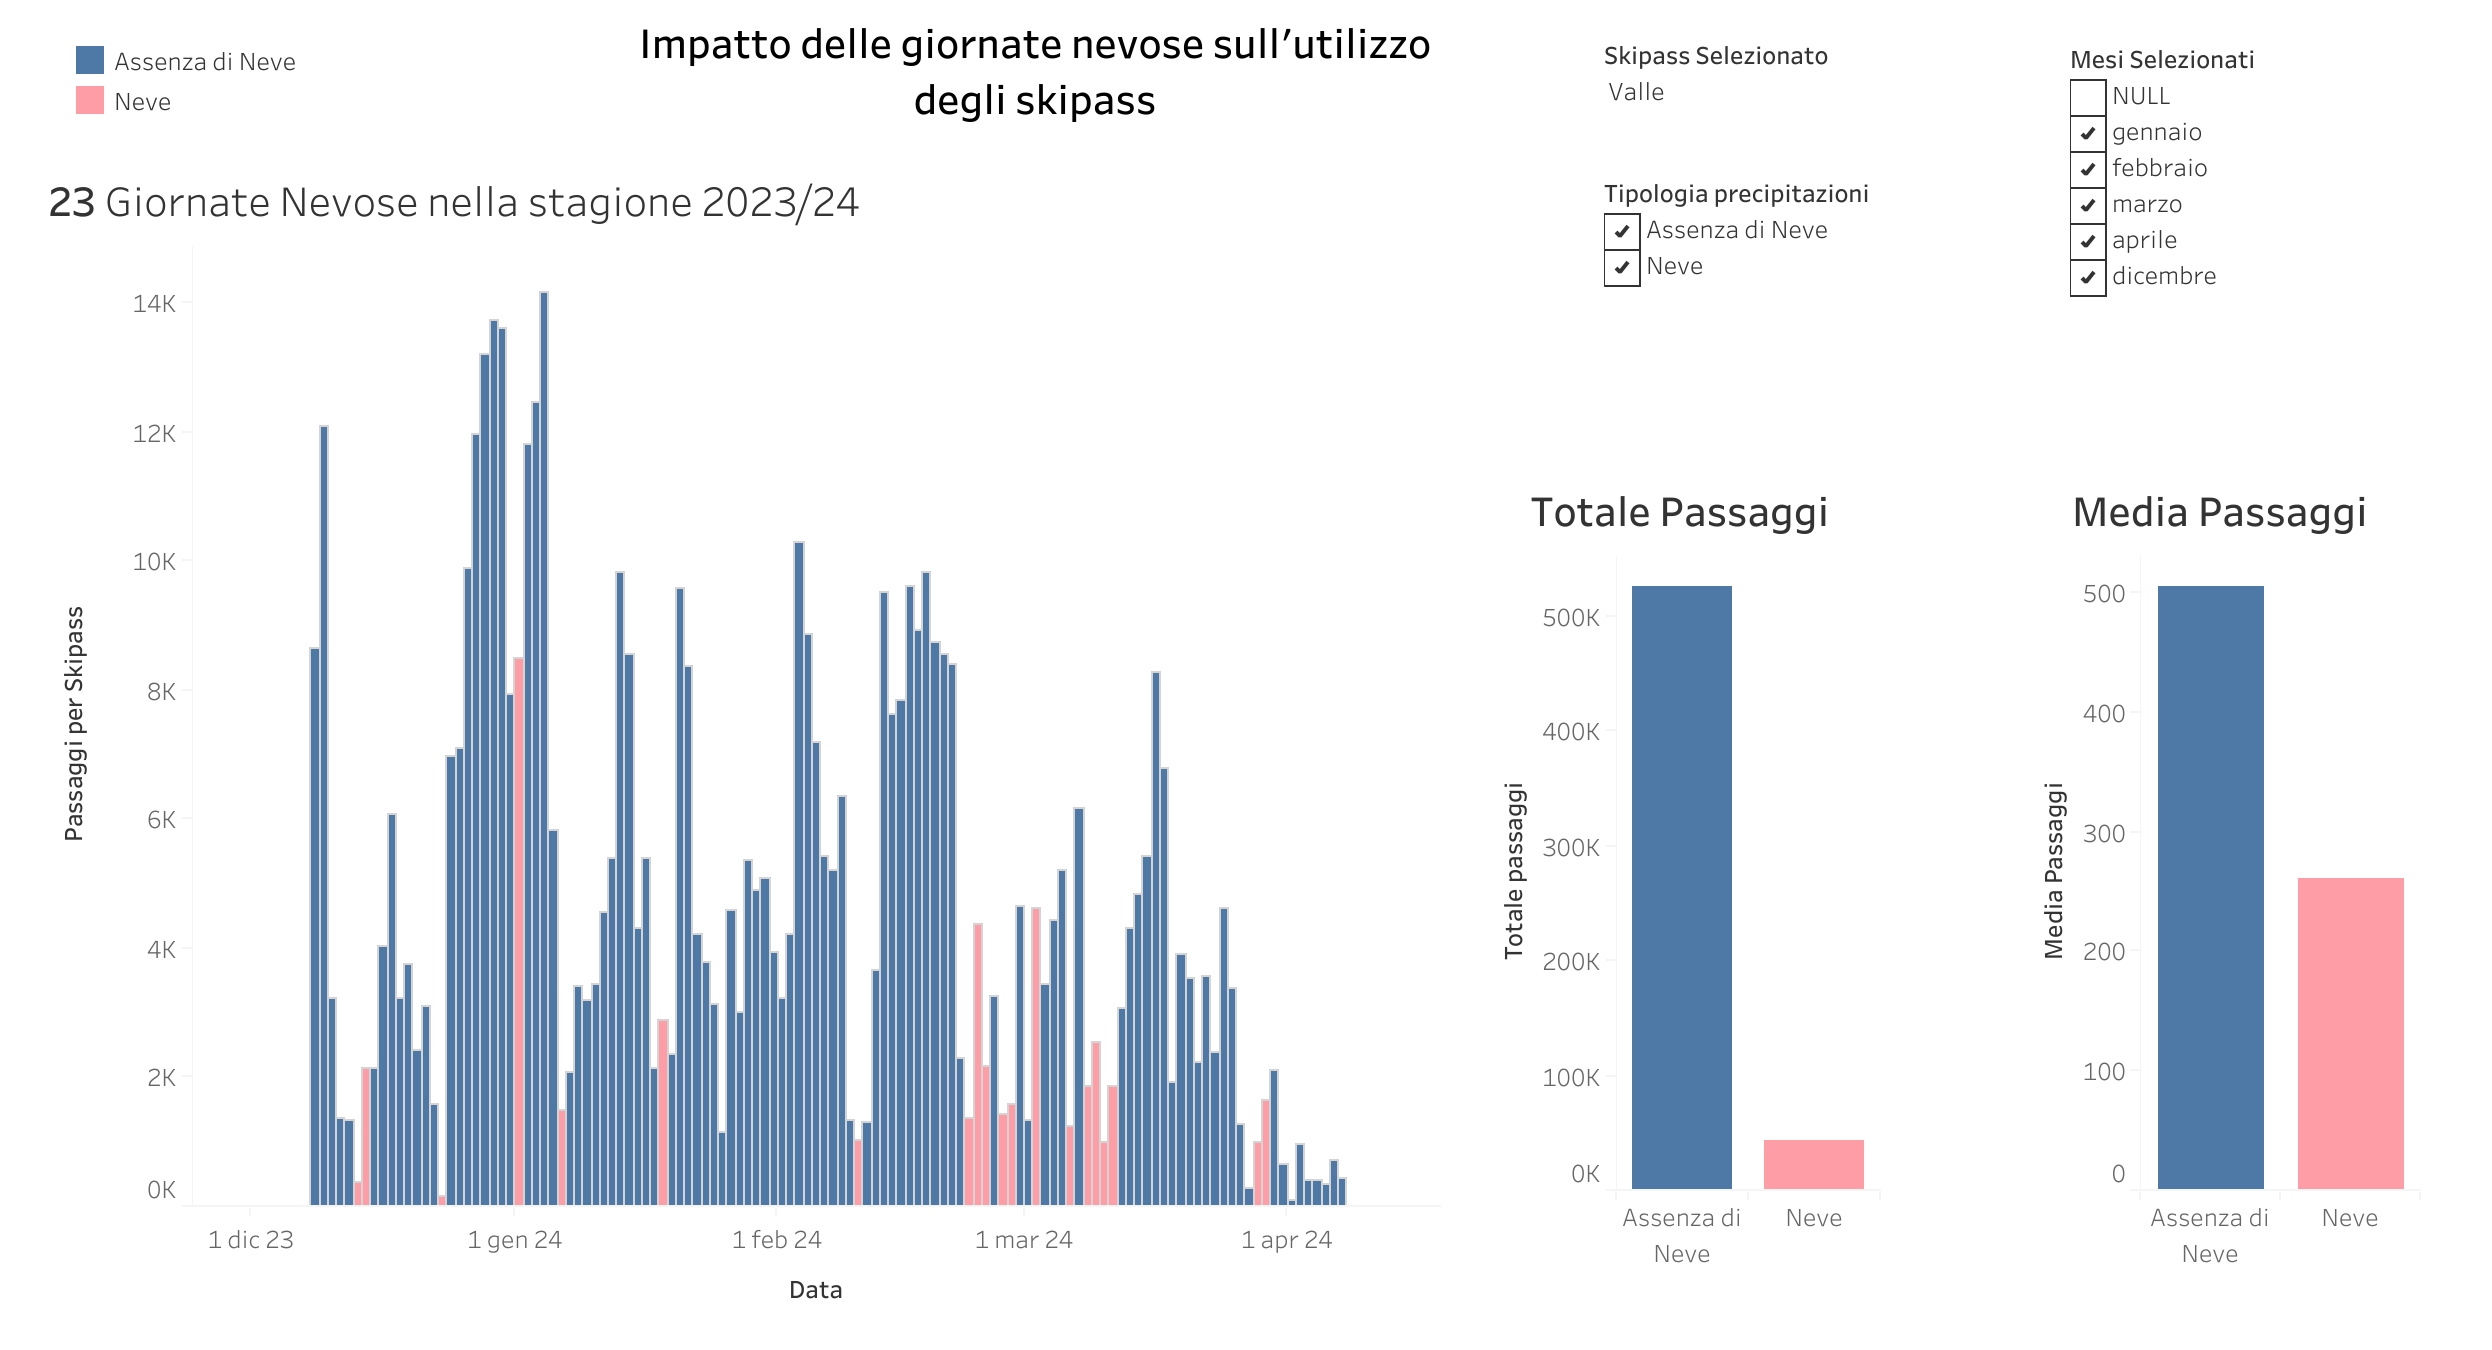
\includegraphics[width=0.95\textwidth]{images/Tableau/Studio_4/Impatto_Neve_valle.png}
    \caption{Dashboard Impatto giornate sull'utilizzo degli Skipass, vista Skipass di Valle}
    \label{fig:Impatto_neve_Valle}
\end{figure}

%\section*{Vista complessiva}
%--Di seguito viene riportata un immagine contenente le 4 dashboard raffigurate nel quarto capitolo dell'elaborato in uan vista unica.

\section*{Vista Completa}
Di seguito viene riportato un \textbf{QR-Code} che rimanda alla pagina dedicata su \textit{Tableau Public}, dove sono raccolte tutte le visualizzazioni interattive e i grafici realizzati per questo elaborato.
L’accesso alla piattaforma consente di esplorare dinamicamente le dashboard, modificare i filtri e approfondire in autonomia le analisi presentate nel capitolo~4\ref{cha:Analisi}.\\

Nella pagina successiva è inoltre inserita un’immagine riepilogativa che mostra le quattro dashboard principali dello studio, offrendo una visione d’insieme delle soluzioni analitiche sviluppate e del loro contributo all’interpretazione dei dati.

\vspace{3cm}
\begin{figure}[htbp]
    \centering
    % Larghezza consigliata: 0.35-0.45 della pagina
    
\includegraphics[width=0.35\textwidth]{images/qr/qr_tableau.png}
    \caption{Visualizzazione Interattiva - Tableau Public}
    \label{fig:qr_tableau}
\end{figure}


\begin{landscape}

\vspace{1em}

\begin{figure}[h]
    \centering
    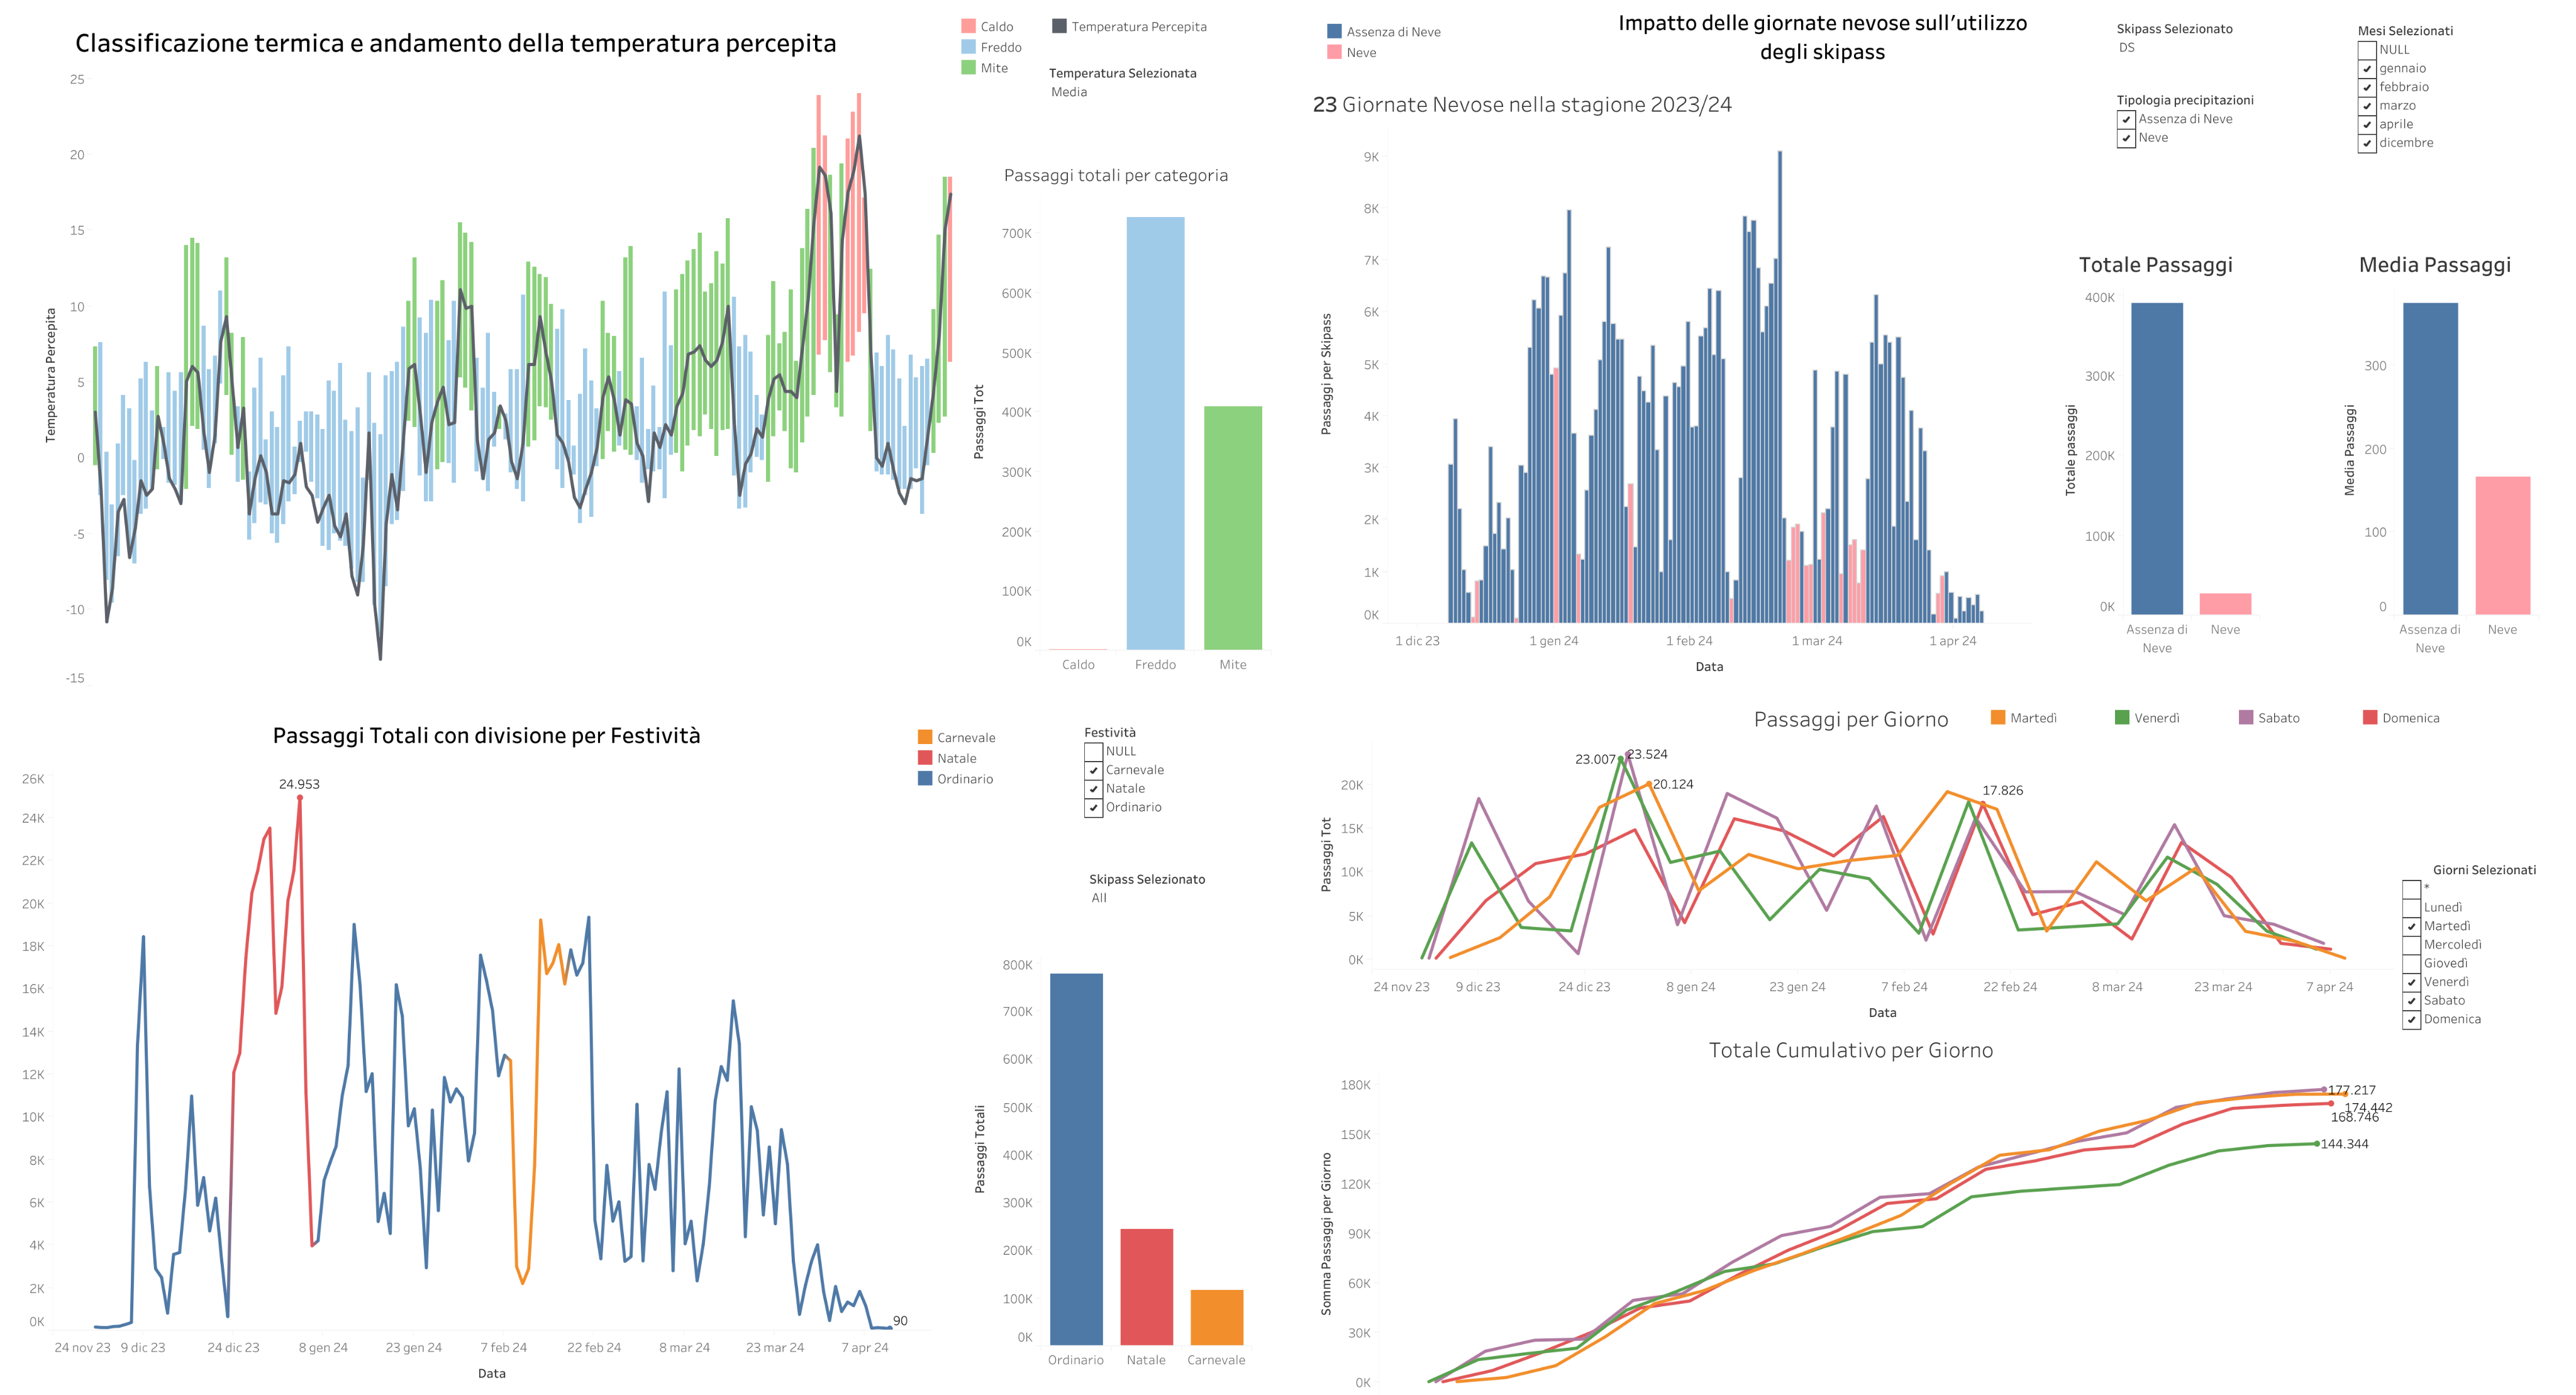
\includegraphics[width=0.95
    \linewidth, height=0.90\textheight]{images/Tableau/dashboard_complessiva.png}
    \caption{Dashboard riunite in un'unica immagine}
    \label{fig:vista_completa}
\end{figure}
\end{landscape}





% --- Pagine bianche finali (per note scritte a mano) ---
\newpage
\thispagestyle{empty}
\mbox{}

\newpage
\thispagestyle{empty}
\mbox{}
% --------------------------
\end{document}
